% !TEX TS-program = lualatex
\documentclass[a4paper, 11pt, fleqn, twoside]{scrreprt}
\usepackage[T1]{fontenc}
\usepackage[english]{babel}
\usepackage{amsmath}
\usepackage{amssymb}
\usepackage[hidelinks]{hyperref}
\usepackage{subcaption}
\usepackage{tikz}
\usepackage{natbib}
\usepackage{abstract}
\usepackage{xcolor}
\usepackage{verbatim}
\usepackage[automark, headsepline]{scrlayer-scrpage}

\RequirePackage[palatino]{quotchap}
\renewcommand*{\chapterheadstartvskip}{\vspace*{-0.5\baselineskip}}
\renewcommand*{\chapterheadendvskip}{\vspace{1.3\baselineskip}}

\setcounter{tocdepth}{1}
\usepackage[titles]{tocloft}
\usepackage[titletoc]{appendix}
\renewcommand{\cftsecleader}{\cftdotfill{\cftdotsep}}
\renewcommand{\cftchapfont}{\normalsize \scshape}
\renewcommand\listfigurename{Listing of figures}
\renewcommand\listtablename{Listing of tables}

\usepackage{fontspec}

\setmonofont{Fira Code Regular}
\setmainfont[ItalicFont={XCharter Italic}]{XCharter Roman}
\newfontfamily{\fallbackfont}{STIX}[Scale=MatchLowercase]
\DeclareTextFontCommand{\textfallback}{\fallbackfont}

\usepackage{newunicodechar}
\newunicodechar{∀}{\textfallback{∀}}
\newunicodechar{≔}{:=}

\usepackage{minted}
\usemintedstyle[Haskell]{trac, fontsize=\small}
\usemintedstyle[Coq]{default, encoding=utf8, fontsize=\small}
\usemintedstyle[Text]{default, fontsize=\small}
%framesep=10pt}

\setmintedinline{style = bw, fontsize=\small, breaklines}

%\AfterEndEnvironment{minted}%
%{\noindent}%

% Für schönere Tabellen (optional)
% \usepackage{booktabs}           % Netteres Tabellenlayout
% \usepackage{multicol}           % Mehrspaltige Bereiche
% \usepackage{tabularx}           % Tabellen mit fester Breite

% Für Listings
% \usepackage{listings}

% Eine kleine Hilfe für offene Lücken
\newcommand{\todo}[1]{\marginpar{\textbf{TODO:} #1}}
\newcommand{\hinl}[1]{\mintinline{Haskell}{#1}}
\newcommand{\cinl}[1]{\mintinline{Coq}{#1}}

\setlength\partopsep{-\topsep}
\addtolength\partopsep{-\parskip}
\addtolength\partopsep{0.32cm}
\raggedbottom

\begin{document}
\pagenumbering{roman} % römische Seitenzahlen

\begin{titlepage}
	\vspace*{3cm}
	\centering
	{\huge\bfseries Modeling Call-Time Choice as Effect using Scoped Free 
	Monads\par}
	\vspace{1cm}
	\textbf{Niels Bunkenburg} \par 
	\vspace{6cm}
	\textbf{Master's Thesis} \par
	Programming Languages and Compiler Construction \par
	Department of Computer Science \par
	Kiel University
	\vfill
	Advised by\par
	P.D. Dr. Frank Huch \par
	M.Sc. Sandra Dylus
	\vfill
	% Randloses Drucken nicht möglich...
	%\tikz[remember picture,overlay] \node[opacity=0.3,inner sep=0pt] at 
	%(9.5,-1.5){
\includegraphics{img/cau-siegel-1400.png}};
	{\large April 2019\par}
\end{titlepage}

\newpage
\thispagestyle{empty}
\strut
\newpage

\chapter*{Erklärung der Urheberschaft}
\vspace{2cm}
Ich erkläre hiermit an Eides statt, dass ich die vorliegende Arbeit ohne Hilfe Dritter und ohne Benutzung anderer als der angegebenen Hilfsmittel angefertigt habe.
Aus fremden Quellen direkt oder indirekt übernommene Gedanken sind als solche kenntlich gemacht.
Die Arbeit wurde bisher in gleicher oder ähnlicher Form in keiner anderen Prüfungsbehörde vorgelegt und auch noch nicht veröffentlicht.

\vspace{4cm}
\hspace{1cm} $\overline{~~~~~~~~~~\mbox{Ort, Datum}~~~~~~~~~~}$ \hfill $\overline{~~~~~~~~~~~~~\mbox{Unterschrift}~~~~~~~~~~~~~}$ \hspace{1cm}

\newpage
\mbox{}
\thispagestyle{empty}
\newpage

\begin{abstract}

\end{abstract}

\newpage
\strut
% This is necessary to apply the command that disables lexer errors for Unicode
\begin{minted}{Coq} 
\end{minted}

\begin{minted}{Haskell}
\end{minted}

% Disable highlighting of lexer errors for Unicode
\makeatletter
\expandafter\def\csname PYGdefault@tok@err\endcsname{\def\PYGdefault@bc##1{##1}}
\makeatother

\makeatletter
\expandafter\def\csname PYGtrac@tok@err\endcsname{\def\PYGtrac@bc##1{##1}}
\makeatother

\thispagestyle{empty}
\newpage

% Verzeichnisse
\renewcommand{\contentsname}{Contents}
%\setcounter{tocdepth}{1}
\tableofcontents   % Inhaltsverzeichnis
%\listoffigures     % Abbildungsverzeichnis
% \listoftables      % Tabellenverzeichnis
% \lstlistoflistings % Abbildungsverzeichnis

\newpage               % Expliziter Umbruch für Seitenzahlen
\strut
\thispagestyle{empty}
\newpage
\pagenumbering{arabic} % arabische Seitenzahlen

% Inhalt

\chapter{Introduction}

Software verification is difficult.
Each day, the amount of software that influences many aspects of our lives -- ranging from communication over socialization to transportation -- grows increasingly.
The results of software that does not behave as intended begin with minor annoyances like a sluggishly responding website and end with catastrophic failures that cost human lives.

Verification techniques like testing, static analysis and formal proofs are an important part of finding programming errors and ensuring that software works as specified.
Although there are no flight control computers running on a functional logic languages like Curry (yet), unique features like non-determinism make Curry an interesting object of software verification.

Verifying the functional language Haskell in Coq, an interactive proof assistant, is a topic of active research, for example by \citet{breitner2018ready} and \citet{dylus2019oneMonad}.
Due to its syntactic resemblance of Haskell, one might assume that Curry can be verified in Coq in a similar matter.
However, some language aspects -- which serve a purely performance-related purpose in Haskell -- interact with Curry's non-determinism in a way that necessitates explicit consideration in the model.

One approach of modeling a programming language in Coq is to translate definitions into equivalent Coq code whenever possible.
Effects, that is, features of a language that surpass pure computation of values, are then modeled by means of other methods and integrated with the translated code.
The result is a combination of native Coq code and modeled effects that, ideally, behaves identical to the original language and can be formally reasoned about.

In the context of Curry, we are interested in \textit{call-time choice}, that is, the interaction between the effects non-determinism and sharing, in combination with non-strict evaluation.
The technique chosen to represent this effect is a combination of representing syntax using the \textit{free monad} and effect handlers that describe the semantics.
Since directly modeling Curry's call-time choice in Coq is complicated by some restrictions that Coq's proof system entails, the model is first implemented in Haskell and then transferred to Coq.

\section{Goals}

The goal of this thesis is to model Curry's call-time choice effect using the effect handler approach.
This includes exploring how effects can be modeled in other languages, for example, how the KiCS2 compiler represents non-determinism when compiling Curry code to Haskell, or how an explicit sharing operator, as introduced by \citet{fischer2009purely}, can be implemented.

Based on the insights obtained in this process, we then want to extend a framework for modeling effects presented by \citet{wu2014effect} to model the call-time choice effect.
Since call-time choice is combined from multiple effects, one of which is a \textit{scoped} effect, we want to investigate how such effects can be implemented.

Finally, when an adequate Haskell model is found, we want to transfer the implementation to Coq in order to verify that the model does not depend on Haskell's non-strictness or built-in sharing.
Furthermore, the last goal of the thesis is to attempt proving the \textit{laws of sharing} defined by \citet{fischer2009purely} for the Coq implementation.

\section{Structure}

The following chapters are structured as follows.
Firstly, we begin with preliminaries in \autoref{ch:preliminaries} about the unique features of Curry and the language Coq.
In addition, an overview of techniques that can be used to represent Curry's non-determinism in Haskell is given.

In \autoref{ch:callTimeChoiceHaskell}, we then have a detailed look at effects and effect handlers, followed by an implementation of sharing as effect.
We explore different approaches and incrementally develop an explicit sharing operator that models Curry's call-time choice semantics.
The chapter is concluded with two exemplary algorithms that make use of non-determinism and sharing.

We begin \autoref{ch:callTimeChoiceCoq} with an explanation of the challenges that transferring the Haskell implementation to Coq poses.
In the following section, a concept is introduced that allows us to represent effects in a different way that Coq accepts.
We discuss the differences of the simplified Coq implementation, compared to Haskell, and how the implementation of the sharing effect can be transferred to Coq.
As an intermediary section, we have a look at how non-strict non-determinism works in Curry and the Coq model.
Finally, a higher-order variation of the previous approach is discussed, together with its strengths and shortcomings.

Second lastly, we discuss program equality and induction principles in  \autoref{ch:progsInCoq}.
Based on this, we then try to prove the laws of sharing for the Coq implementation.

The last \autoref{ch:conclusion} summarizes the approach and findings of the thesis.
An overview of related work is given and future work is discussed.

\chapter{Preliminaries}
\label{ch:preliminaries}
This chapter introduces the languages Curry and Coq as well as the modeling methods that are applied in the next chapters of the thesis.
A sufficient understanding of functional programming languages like Haskell and the underlying concepts -- such as algebraic data types, polymorphism, type classes and monads -- is assumed.


\section{Curry}
Curry \citep{hanus2016curry} is a functional logic programming language based on Haskell.
Its syntax is therefore largely based on Haskell's and many features like pattern matching, polymorphism, higher-order functions and type classes are supported in Curry, too.
Besides its functional part, Curry incorporates logical aspects known from languages like Prolog.
These include non-determinism and free variables, that is,  multiple values as the result of evaluating an expression and a representation of unknown values.

Curry programs can be executed using one of many compilers.
Most notable are KiCS2\footnote{\url{https://www-ps.informatik.uni-kiel.de/kics2/}} and PAKCS\footnote{\url{https://www.informatik.uni-kiel.de/~pakcs/}}, which compile Curry code into Haskell and Prolog programs, respectively.
Due to Curry's similarity to Haskell, only unique features that are relevant for this thesis are discussed, beginning with the three core properties that make up call-time choice.

\subsection{Non-Strictness}
Usually when the evaluation of a subexpression fails, the whole expression fails, too.
The so-called strict semantics is the idea behind the evaluation strategy of most modern languages.
However, certain aspects of strict languages like conditional branching need to be evaluated non-strictly because otherwise loops would otherwise not terminate.

In contrast, it is also possible to give a whole language non-strict semantics, as evidenced by Haskell and Curry.
This means that an expression may have a value, although some subexpressions are not evaluated yet.
Consequently, non-strictness allows defining conceptually infinite data structures like a list of all powers of two.

\begin{minted}{Haskell}
pow2s :: [Int]
pow2s = 1 : map (2*) pow2s
\end{minted}

Although this list is infinite and cannot be evaluated wholly, non-strictness allows us to evaluate only the parts that are demanded by the surrounding expressions.

\begin{minted}{Haskell}
λ> take 4 pow2s
[1,2,4,8]
\end{minted}

Non-strict semantics can be implemented using an outermost evaluation strategy.
This means that the reducible term closest to the root of the expression is evaluated first.
For example, \hinl{take 2 pow2s} is evaluated using an outermost strategy as follows.

\begin{minted}{Haskell}
  take 2 pow2s
= take 2 (1 : map (2*) pow2s)
= 1 : take 1 (map (2*) pow2s)
= 1 : take 1 (map (2*) (1 : (map (2*) pow2s)))
= 1 : take 1 (2 * 1 : map (2*) (map (2*) pow2s))
= 1 : 2 : take 0 (map (2*) (map (2*) (1 : map (2*) pow2s)))
= 1 : 2 : []
= [1, 2]
\end{minted}

The example shows the concept of alternating production and consumption of data.
When \hinl{take} cannot consume a list element because its second argument is not in head normal form, that is, the root expression is not a constructor or lambda abstraction, \hinl{pow2s} is evaluated to produce the demanded list element.
This process repeats for the second element.
When the first argument of \hinl{take} reaches zero, the list argument is not evaluated further and the empty list is returned.
Consequently, it does not matter if a function has an argument whose evaluation would fail, as long as the value is not evaluated by the function.
For example, \hinl{const 42 (head [])} has the value \hinl{42} in Curry and Haskell.

\subsection{Non-Determinism}
Evaluating expressions in Haskell is deterministic, that is, an expression evaluates to exactly one result.
Since it is possible to define functions with overlapping patterns, Haskell uses only the first matching rule to determine the result of a computation.
In Curry, however, this restriction is not present.
If multiple patterns match an expression, the computation becomes non-deterministic and each applicable rule returns a result.
The most simple, but very useful non-deterministic function is the choice operator, which is defined as follows.

\begin{minted}{Haskell}
(?) :: a -> a -> a
x ? _ = x
_ ? y = y
\end{minted}
\noindent
Both rules match for any input, so \hinl{0 ? 1} yields both \hinl{0} and \hinl{1} as results.

Non-deterministic functions do not differ from deterministic ones in regard to the type system because there is no special syntax to denote this property in the signature.
Although it is necessary to inspect the definition of a function in order to determine whether it is non-deterministic, we can freely combine deterministic and non-deterministic functions this way.
When a deterministic function is applied to a non-deterministic argument, the function becomes non-deterministic itself.

\begin{minted}{Haskell}
λ> even (0 ? 1)
True
False
\end{minted}

However, this effect is limited by non-strictness.
If a function does not evaluate the non-determinism contained in one of its arguments, the function remains deterministic.
For example, \hinl{const 42 (0 ? 1)} only yields \hinl{42}.

Besides multiple values as the result of evaluating a non-deterministic expression, failure is also a valid option.
There are two kinds of failures in Curry: silent failures as part of a non-deterministic computation and top-level failures.
The former is shown in the following example.

\begin{minted}{Haskell}
λ> head ([] ? [1])
1
\end{minted}

The choice operator in the argument of \hinl{head} makes the function non-deterministic.
Whereas the first choice branch fails, the second one succeeds and returns the value \hinl{1}.
Although one computation failed, this is not apparent from the result, unless the failure happens at top-level.
In this case, the whole computation fails.

\subsection{Sharing}
The last aspect of call-time choice is sharing, that is, computing the result of an expression only once even if it is used multiple times.
When a variable is introduced via a pattern or local binding, each occurrence of the variable in an expression acts as a pointer to the same computation.
Due to referential transparency, it does not make a difference if or how many times an expression is recomputed.
Thus, sharing does not affect the semantics in Haskell.
In Curry, however, non-determinism can occur in shared expressions, for example as follows.

\begin{minted}{Haskell}
double :: Int -> Int
double x = x + x
\end{minted}

When \hinl{double} is called with a non-deterministic argument, there are two possible options: Firstly, the choices in both occurrences of \hinl{x} can behave independently of each other, which is called run-time choice.
Secondly, there is call-time choice.
Conceptually, call-time choice means that the decision of which branches are taken in a non-deterministic argument are determined at the time the function is called.
Of course this does not mean that the argument is evaluated before the function is called.
Instead, sharing that is introduced by the pattern variable of a function means that, whenever a decision is made in any occurrence of the shared variable, the same decision must be made in all other occurrences of said variable.
Consequently, sharing that is introduced by pattern variables can be transformed into local bindings.

\begin{minted}[escapeinside=<>]{Haskell}
  double (0 ? 1) 
<$=$> let x = 0 ? 1 in x + x 
<$\neq$> (0 ? 1) + (0 ? 1)
\end{minted}

However, replacing the occurrences of a variable with the shared expression gives the function call different semantics because the choices become independent of each other.
Whereas both expression with shared non-determinism return only \hinl{0} and \hinl{2} because the decisions are made uniformly, the last expression evaluates to \hinl{0}, \hinl{1}, \hinl{1} and \cinl{2} since both terms of the sum can be \hinl{0} and \cinl{1}, independent of each other.

With non-strictness, non-determinism and sharing as the main components of call-time choice, we have discussed the main aspects we want to model.
In the next section, we focus on a language that allows us to formally reason about such a model.

\section{Coq}
\label{sec:coqIntro}

Coq is an interactive proof assistant created by \citet{coq2019}.
At its core, Coq consists of the functional, dependently typed specification language \textit{Gallina} and the proof tactic language L$_\text{tac}$.
Gallina programs are structured as sentences of \textit{The Vernacular} commands, where each sentence begins with a capital letter and ends with a dot.
Sentences are processed sequentially, that is, from top to bottom of the file.

The most actively developed tools for programming in Coq are CoqIDE, a standalone editor developed together with the language, and the Emacs package Proof General\footnote{\url{https://proofgeneral.github.io/}} or its extension Company-Coq\footnote{\url{https://github.com/cpitclaudel/company-coq}}.
The latter is shown in the \autoref{fig:company-coq}.
The interface is split into two main parts: The left-hand side shows the program and current progress, where loaded sentences are colored in light blue.

\begin{figure}
\begin{center}
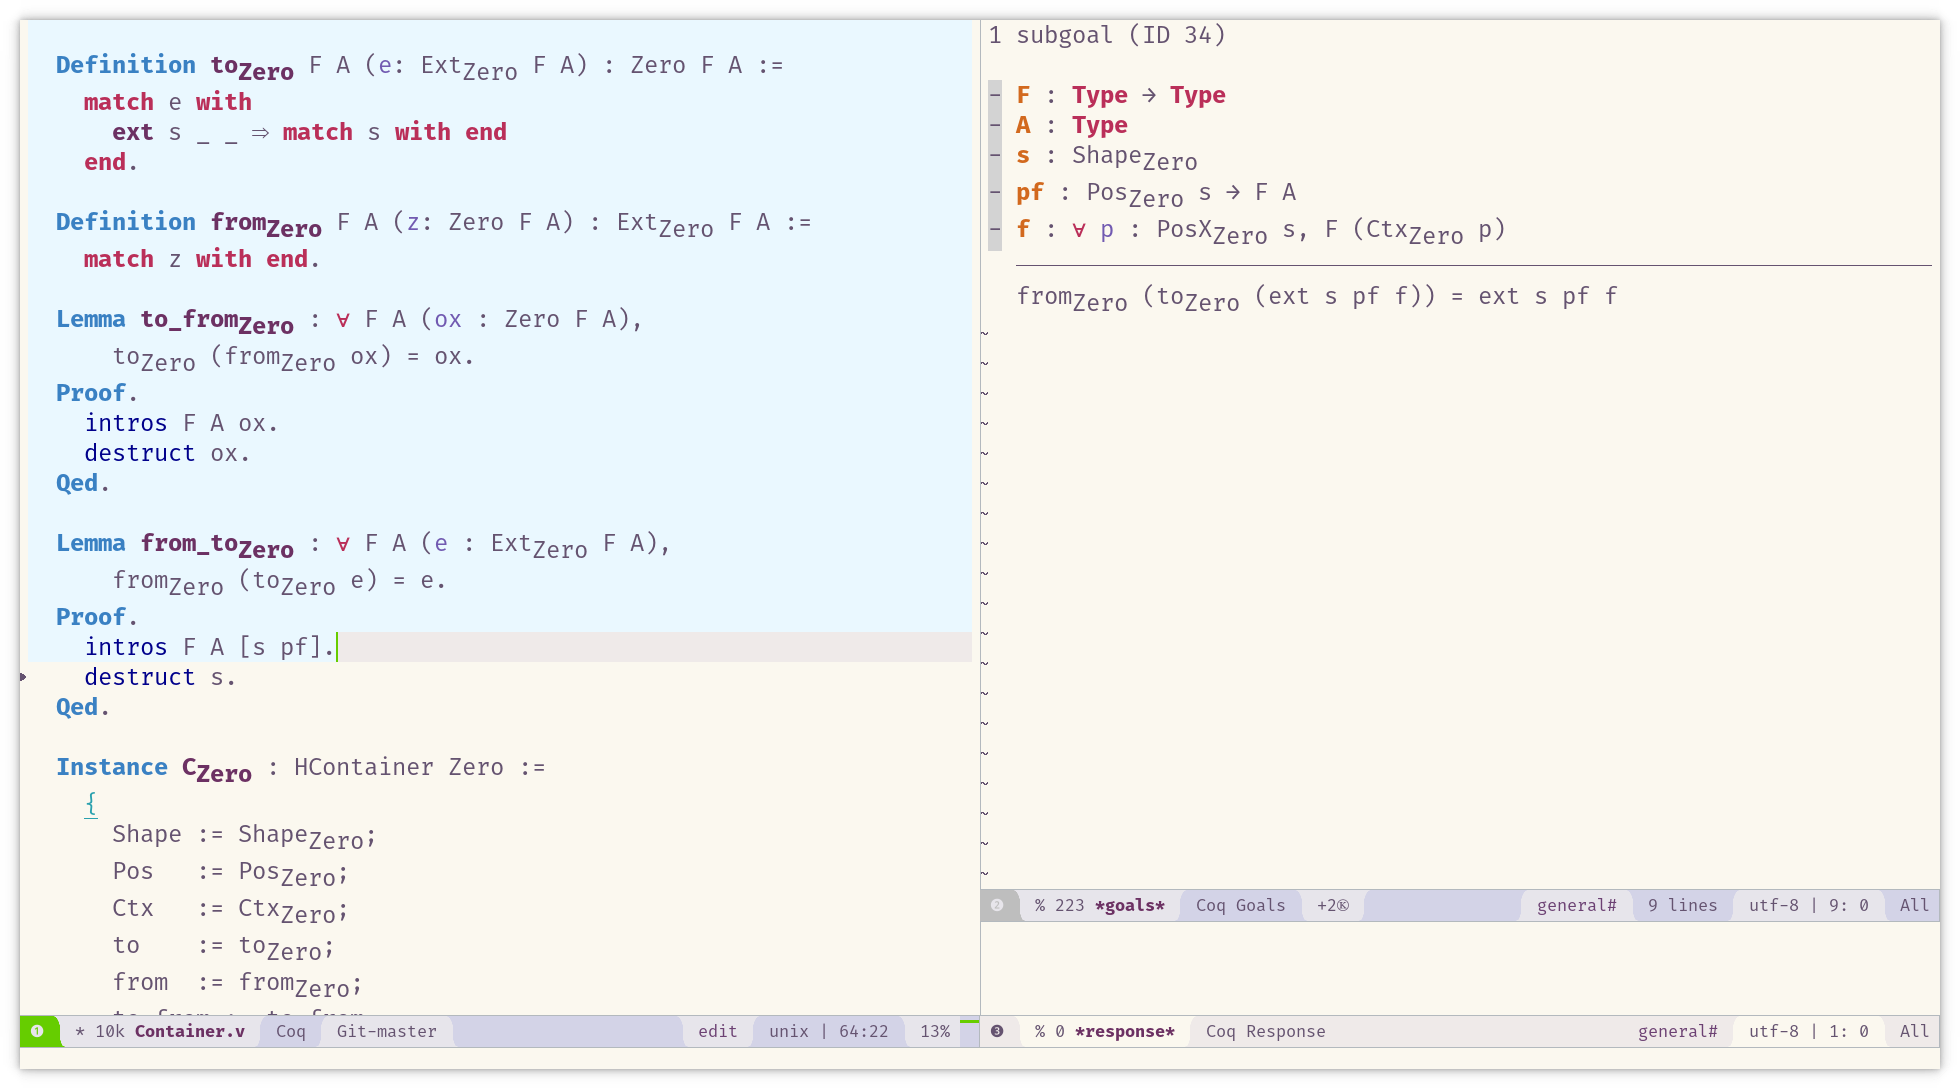
\includegraphics[width=\textwidth]{img/coq.png}
\end{center}
\caption{Interface of the Company-Coq package for Emacs}
\label{fig:company-coq}
\end{figure}


The lower right-hand side region of the screen shows errors and other messages, while the upper part is used for proofs.
The proof context, that is, all variables that have been introduced so far, is shown at the top.
Separated by a line, the current goal follows below the context.

In the following, an introduction to the syntax and concepts of Coq is given.

\subsection{Data Types}
\label{subsec:coqdatatypes}
One important aspect of functional programming languages is the ability to easily define new data types.
In Coq, constructor-based data types are defined using the keyword \cinl{Inductive}, which is followed by the name of the type and a list of type arguments.
After a colon, the type of the definition follows.
For inductive definitions like \cinl{option}, this type is \cinl{Type}.

\begin{minted}{Coq}
Inductive option (A : Type) : Type := 
| Some : A -> option A 
| None : option A.
\end{minted}

The \cinl{option} type is the predefined equivalent to the \hinl{Maybe} type in Haskell.
Constructors of inductive data types are defined by giving the full type.
Based on this definition, we can define values of \cinl{option} like \cinl{Some nat 42} or \cinl{None bool}.

By default, all arguments -- including type variables -- need to be specified when using polymorphic data types.
However, the command \cinl{Set Implicit Arguments} can be used to enable Coq's ability to infer values that can be derived directly from other arguments.
Now we can omit the type argument of \cinl{Some} because the type \cinl{A} can be inferred from the supplied value.

Based on the \cinl{option} type, we can define a list type that has optional components as follows.
\begin{minted}{Coq}
Inductive List A : Type :=
| Nil  : List A
| Cons : option A -> option (List A) -> List A.
\end{minted}

Since \cinl{option} is applied to \cinl{List} in the second constructor, this kind of definition is called \textit{nested inductive}.
Although we have enabled implicit arguments, we still have to give an explicit type argument to \cinl{Nil}, as shown in the following example.

\begin{minted}{Coq}
Check Cons (Some 42) (Some (Nil nat)).
  : List nat
\end{minted}

The type argument of \cinl{Nil} cannot be inferred yet because no argument of \cinl{Nil} holds information about \cinl{A}.
Nevertheless, the type argument can be inferred from the context of \cinl{Nil}, where \cinl{A} is defined as \cinl{nat} by the first argument of \cinl{Cons}.
Such contextual inference of values can be enabled with the command \cinl{Set Contextual Implicit}.
Now we can use \cinl{List} without explicit type arguments.

In some situations, the type inference is not able to gather all required information.
For example, defining \cinl{Cons None None} leads to the error message 'Cannot infer the implicit parameter \cinl{A} of \cinl{Cons} whose type is \cinl{Type}'.
Thus, it is possible to explicitly pass implicit parameters by adding \cinl{@} in front of the function or constructor name.
\begin{minted}{Coq}
Definition empty A := @Cons A None None.
\end{minted}

\subsection{Functions}
\label{subsec:coqFunctions}

Based on data types, we can define functions that process data.
The keyword \cinl{Definition} is predominantly used to define values, types and non-recursive functions.
Since data types and functions defined in Gallina are the input of Coq's proof verification logic, the specification language only allows provably terminating definitions.
Consequently, Coq distinguishes recursive and non-recursive functions by means of an explicit \cinl{Fixpoint} operator for functions of the former kind.
As an example of a simple non-recursive function, we define the function \cinl{head} for the \cinl{List} type.

\begin{minted}{Coq}
Definition head A (oxs : List A) : option A :=
  match oxs with
  | Nil       => None
  | Cons ox _ => ox
  end.
\end{minted}

Similar to data types, all occurring type variables need to be introduced explicitly in the function head.
Pattern matching in Coq is done using the \cinl{match} construct.
All functions must be total and thus, if an argument is matched, the patterns must be exhaustive.
Since the elements of \cinl{List} are optional by definition, the return type is, too.
Therefore, it is possible to define \cinl{head} for \cinl{List}.
A partial function like \cinl{head} for ordinary lists in Haskell cannot be defined in Coq.
However, it is possible to define lists in a different way that circumvents this problem, as described in \autoref{subsec:dependent}.

As an example of recursive functions, we define an append function over \cinl{List}.
Similar to the situation we encounter later in \autoref{ch:callTimeChoiceCoq}, the \cinl{List} arguments are wrapped in \cinl{option} types because optional components alone are not sufficient to model some aspects of call-time choice.

\begin{minted}{Coq}
Fail Fixpoint app A (oxs oys : option (List A)) : option (List A) :=
  match oxs with
  | None    => None
  | Some xs =>
    match xs with
    | Nil         => oys
    | Cons oz ozs => Some (Cons oz (app ozs oys))
    end
  end.
\end{minted}

As indicated by \cinl{Fail}, this definition fails to load in Coq with the error message 'Cannot guess decreasing argument of fix'.
Such errors generally mean that Coq is not able automatically detect that a recursive function always terminates.
The reason for this requirement is explained in more detail in \autoref{sec:non-strictly}.
In short, Coq's termination checker ensures that the proof logic remains sound.
However, the termination check is too restrictive in some situations, as evidenced by \cinl{app}.
Since the recursive call of \cinl{app} has \cinl{ozs} as its first argument, which is a subterm of \cinl{xs} and, consequently, \cinl{oxs}, the function is always called with structurally smaller values, which implies that the function eventually terminates.
Unfortunately, Coq is not able to track subterms across multiple levels of pattern matching in combination with nested inductive types. \citet{chlipala2013certified} describes this topic as follows.

\begin{quotation}
\noindent
There is no deep theoretical reason why this program should be rejected; Coq applies incomplete termination-checking heuristics, and it is necessary to learn a few of the most important rules. The term "nested inductive type" hints at the solution to this particular problem[:] [\dots{}] nested types require nested recursion.
\end{quotation}

In the example of \cinl{app}, nested recursion is not necessary, because option is not a recursive type.
The basic idea, however, still applies.
Instead of defining a single function that handles the nested patterns of a nested type, we split the function into two parts.
First, however, we generalize the first \cinl{match} expression over optional values into the function \cinl{bind}.

\begin{minted}{Coq}
Definition bind A B (o : option A) (f : A -> option B) : option B :=
  match o with
  | None   => None
  | Some x => f x
  end.
\end{minted}

Now we remove the \cinl{option} wrapper from the first \cinl{List} argument and reuse the remaining definition except for the second argument of \cinl{Cons}.

\begin{minted}{Coq}
Fixpoint app' A (xs : List A) (oys : option (List A)) 
  : option (List A) :=
  match xs with
  | Nil         => oys
  | Cons oz ozs => Some (Cons oz (bind ozs (fun zs => app' zs oys)))
  end.
\end{minted}

Since \cinl{app'} expects an argument of type \cinl{List A} but the second argument of \cinl{Cons} has the type \cinl{option (List A)}, we use \cinl{bind} to retrieve the list \cinl{zs} for the recursive call.
Now we can define the last remaining part of the function, that is, a definition that has the original type of \cinl{app} and uses \cinl{app'}, with the help of bind.

\begin{minted}{Coq}
Definition app A (oxs oys : option (List A)) : option (List A) :=
  bind oxs (fun xs => app' xs oys).
\end{minted}

These three definitions are all accepted by Coq and allow us to define recursive functions over nested inductive types.

Another example of a recursive function that Coq's termination check does not accept is the Quicksort algorithm.
Using the predefined \cinl{filter} function and Boolean comparison operator \cinl{leb} as well as Boolean negation, the function could look as follows.
To define the predicate arguments of \cinl{filter}, we use anonymous functions, which are defined in Coq using the keyword \cinl{fun}.

\begin{minted}{Coq}
Fail Fixpoint quicksort (xs : list nat) : list nat :=
  match xs with
  | nil       => nil
  | cons y ys =>
    let le := fun x => Nat.leb x y in
    let gt := fun x => negb (Nat.ltb x y)
    in quicksort (filter le ys) ++ [y] ++ quicksort (filter gt ys)
  end.
\end{minted}

This definition is not accepted by Coq because the argument of the recursive call is modified by another function and thus, is not necessarily structurally decreasing.
Nevertheless, there is a way to define such functions, which leads to the next subsection.

Using \cinl{Program Fixpoint}, which is special syntax that can be imported using the command \cinl{Require Import Program}, we split the definition into two parts.
The first part is almost the same definition as before, except for an additional argument called \textit{measure}.
This value is used as evidence that the function is called with structurally decreasing arguments.
In the case, we use \cinl{length xs} as measure, because each call of \cinl{quicksort} splits the input list into two structurally smaller lists.

The second part of a \cinl{Program Fixpoint} definition are proof obligations that are automatically generated based on the function definition and the supplied measure.
Since we have not yet discussed how proofs in Coq work, this is the topic of the next subsection.

\subsection{Propositions and Proofs}

The goal of a proof in Coq is to construct evidence that a certain proposition holds.
Propositions have the type \cinl{Prop} and represent statements about Gallina structures.
For example, $1 = 0$ is a proposition, although not a provable one.

The term 'constructing evidence' is related to the \textit{Curry-Howard Correspondence}, which suggests that logical proofs and computational values are strongly connected.
When we reason mathematically about a statement like $1 = 1$, we might argue that equality is a reflexive relation and thus, the statement must be true.
We can do the same in Coq as follows.

\begin{minted}{Coq}
Lemma eq11 : 1 = 1.
Proof. reflexivity. Qed.
\end{minted}

Proofs in Coq start with the command \cinl{Proof} and end with \cinl{Qed}.
L$_\text{tac}$ tactics like \cinl{reflexivity} represent values that Coq constructs in the background when a proof is defined.
The constructed value can be printed using \cinl{Print eq11}, which yields the following.

\begin{minted}{Coq}
Print eq11.
  eq_refl : 1 = 1
\end{minted}

When we talk about values in the context of proofs, the type operator \cinl{:} can be read as 'is a proof of', that is, \cinl{eq_refl} is a proof of \cinl{1 = 1}, in this case.
In order to find out more about \cinl{eq_refl}, we can ask Coq for the definition of the equality operator, using \cinl{Locate} and then \cinl{Print}.

\begin{minted}{Coq}
Locate "=".
  Notation
  "x = y" := eq x y : type_scope (default interpretation)

Print eq.
  Inductive eq (A : Type) (x : A) : A -> Prop :=  eq_refl : x = x
\end{minted}

Now we know that \cinl{=} is a notation for the \textit{inductively defined proposition} \cinl{eq}.
'Inductively defined' means that a proposition consists of multiple constructors whose definition is usually related to the inductive data type that the proposition reasons about.
The constructor \cinl{eq_refl} matches values of all types and can be applied if its first argument \cinl{x} and second argument -- the argument of type \cinl{A} that follows -- are the same.
Since this is the case in our example, the value \cinl{eq_refl} proves the proposition.

Based on this first idea of Coq's proof logic, we can now return to the QuickSort example and discuss the termination proofs.
Before we begin, we consider properties of \cinl{filter} that might be useful in the proofs.
For example, when we filter a list \cinl{xs} with an arbitrary predicate \cinl{p}, the resulting list should always be smaller or at most equally long as \cinl{xs}.

\begin{minted}{Coq}
Lemma filter_length: forall (A : Type) (xs : list A) (p : A -> bool),
  length (filter p xs) <= length xs.
Proof.
  intros A xs p.
  induction xs; simpl.
  - reflexivity.
  - destruct (p a); simpl.
    + apply le_n_S.
      apply IHxs.
    + apply le_S.
      apply IHxs.
Qed.
\end{minted}

When a tactic yields multiple subgoals, the symbols \cinl{-}, \cinl{+} and \cinl{*} can be used to structure the proof.
We begin the proof with \cinl{intros A xs p}. 
This command moves quantified variables from the goal to the context.
Hence, the proof view now looks as follows.

\begin{minted}{Coq}
A : Type
xs : list A
p : A -> bool
============================
length (filter p xs) <= length xs
\end{minted}

To further advance the proof, we need more information about \cinl{xs}, because both \cinl{length} and \cinl{filter} do pattern matching.
For inductive data types, the tactic \cinl{destruct} does a case distinction over the constructors of the passed argument, where each constructor generates one new subgoal.
For non-recursive data types like \cinl{bool}, this is sufficient.
However, proofs over recursive data types like \cinl{list} usually require structural induction to be able to prove the property.
Consequently, we use \cinl{induction xs} to distinguish empty lists and non-empty lists.

When a semicolon is used instead of a dot between two tactics, the second tactic is applied to all subgoals that the first one generates.
In this case, we want to apply the tactic \cinl{simpl} to both cases and thus, combine \cinl{induction xs} and \cinl{simpl} with a semicolon.
The tactic \cinl{simpl} tries to reduce an expression while still maintaining readability.
For example, \cinl{simpl} applies the definition of \cinl{filter} and \cinl{length} because the outermost constructor of \cinl{xs} has been determined by \cinl{induction}.
In the following goal, \cinl{::} is an infix notation for the \cinl{cons} constructor.

\begin{minted}{Coq}
subgoal 1 (ID 63) is:
  0 <= 0
subgoal 2 (ID 64) is:
 length (if p a then a :: filter p xs else filter p xs) 
  <= S (length xs)
\end{minted}

For the first subgoal, which corresponds to the case \cinl{xs = nil}, the functions on both sides of the inequality have been reduced to \cinl{0}.
Since \cinl{<=} is a reflexive relation, this goal is solved trivially.
In the second subgoal, the definition of \cinl{filter} and \cinl{length} have been applied once.
Additionally, the induction hypothesis created by the \cinl{induction} tactic is added to the context.

\begin{minted}{Coq}
A : Type
a : A
xs : list A
p : A -> bool
IHxs : length (filter p xs) <= length xs
============================
length (if p a then a :: filter p xs else filter p xs)
<= S (length xs)
\end{minted}

Again, we need to make a case distinction, but this time over the result of \cinl{p a}.
Since \cinl{bool} is not a recursive type, the tactic \cinl{destruct} applied to \cinl{p a} is sufficient.
In case of \cinl{p a = true}, the new goal is \cinl{ S (length (filter p xs)) <= S (length xs)}.
When compared to the induction hypothesis \cinl{IHxs}, the only difference are the \cinl{S} constructors.
Since they can be removed without affecting the inequality, we ask Coq if such a proposition already exists by means of \cinl{Search (S _ <= S _)}, where underscores represent a wildcard pattern.
The result is the following lemma.

\begin{minted}{Coq}
le_n_S: forall n m : nat, n <= m -> S n <= S m
\end{minted}

The lemma can be applied with the tactic \cinl{apply}.
In general, \cinl{apply} works by matching the goal against the conclusion $c$ of a lemma of type $p_1 \rightarrow \dots \rightarrow p_n \rightarrow c$ where $p$ represent premises.
When the matching is successful, a new subgoal for each premise is generated.
Thus, \cinl{apply} 'reasons backwards' in the sense that we replace the current goal with premises, which, if eventually proven, imply that the original goal must hold, too. 
In this case, the only premise is \cinl{n <= m}.
Therefore, the new goal is identical to the induction hypothesis, which can be applied with \cinl{apply}, too.

For the second case that corresponds to \cinl{p a = false}, the reasoning is similar to the first case but with a slightly different lemma.
This concludes the proof of the helper lemma \cinl{filter_length} and allows us to finally begin the termination proofs for Quicksort.

Using the command \cinl{Next Obligation}, we can begin the first of two termination proofs, where each one corresponds to one recursive call.
The proof context and goal now looks as follows.

\begin{minted}{Coq}
y : nat
ys : list nat
============================
length (filter (fun x : nat => Nat.leb x y) ys) < S (length ys)
\end{minted}

In the proof context, we have an element \cinl{y} and a list \cinl{ys} of natural numbers.
After simplifying the expression, the goal is to show that a filtered list is smaller than the length of the original list plus one.
Using Coq's search, we find the following lemma that allows us to transform the current goal into an inequality over \cinl{<=}.

\begin{minted}{Coq}
Lt.le_lt_n_Sm: forall n m : nat, n <= m -> n < S m
\end{minted}

This leads to the following goal.

\begin{minted}{Coq}
length (filter (fun x : nat => Nat.leb x y) ys) <= length ys
\end{minted}

Coincidentally, the remaining goal can be proven directly using the helper lemma \cinl{filter_length}.

The second termination proof is identical to the first one because the helper lemma holds for any predicate, which is the only difference between both recursive calls.
Finally, we have defined the function using \cinl{Program Fixpoint} and two termination proofs.
Since there is no \hinl{ghci}-like REPL for Coq, we can ask Coq to compute the value of an expression using the command \cinl{Compute} as part of the program.

\begin{minted}{Coq}
Compute quicksort [23; 8; 15; 4; 42; 16].
  = [4; 8; 15; 16; 23; 42] : list nat
\end{minted}

In conclusion, we have seen two kinds of definitions that Coq's termination checker does not accept and two ways to bypass these restrictions.

\subsection{Dependent Types}
\label{subsec:dependent}

Since Coq is a dependently typed language, it is also possible to have values as part of the type.
For example, the following definition represents a list data type -- also called vector -- that encodes the list's length in the type using Peano numbers.

\begin{minted}{Coq}
Inductive vec (A : Type) : nat -> Type :=
| vnil  : vec A 0
| vcons : forall n, A -> vec A n -> vec A (S n).
\end{minted}

The constructor \cinl{vnil} is a vector of length zero, whereas \cinl{vcons} has an explicit argument \cinl{n} introduced by \cinl{forall} that represents the length of the vector's tail.
Since the tail has length $n$ and an element is added, the whole vector has $n + 1$ elements, represented by the successor constructor.
Using this inductive definition of vectors, we can write a singleton vector of Boolean values as \cinl{vcons bool 0 true (vnil bool)}.
When we enable Coq's inference capabilities as described in \autoref{subsec:coqdatatypes}, this value can be defined as \cinl{vcons true vnil}.
As a non-recursive function over vectors, we define a length function as follows.

\begin{minted}{Coq}
Definition vlength (A : Type) (n : nat) (xs : vec A n) : nat := n.
\end{minted}

In this case, the length parameter encoded in the vector type is also a parameter of the function and the result of the function.
Although this might seem strange because the result of the function is also a parameter, it makes sense when we consider that parameters, whose value can be inferred from other arguments, can be omitted.

\begin{minted}{Coq}
Compute vlength (vcons true (vcons true vnil)).
     = 2 : nat
\end{minted}

When we enable explicit arguments for \cinl{vlength} and supply a value for \cinl{n} that does not match the length of the vector, Coq yields a type error.

\begin{minted}{Coq}
Compute @vlength bool 2 (vcons true vnil).
     Error: The term "vcons true vnil" has type "vec bool 1"
              while it is expected to have type "vec bool 2".
\end{minted}

As an example of a recursive function, we define the append function for vectors.
Again, there is a type argument and two natural numbers that represent the lengths of the respective vectors.
The encoded length argument allows us to express the invariant that appending two vectors of length $n$ and $m$ yields a vector with $n + m$ elements.

\begin{minted}{Coq}
Fixpoint vapp (A : Type) (n m : nat) (xs : vec A n) (ys : vec A m) 
  : vec A (n + m) :=
  match xs with
  | vnil       => ys
  | vcons z zs => vcons z (vapp zs ys)
  end.
\end{minted}

As discussed in the previous section, it is not possible to define a function that returns the head of an ordinary list without a wrapper like \cinl{option} because functions must be total.
However, for dependently typed vectors, it is possible to ensure that the function is only applied to non-empty vectors.

Functions over dependent types can be tricky to write directly in some situations.
In the last subsection, the Curry-Howard correspondence and values as proofs were discussed.
In the context of dependent types, the other direction, that is, proofs as values, are more interesting.
Using Coq's proof mode, we are able to define computational functions with proof tactics as follows.

\begin{minted}{Coq}
Definition vhead (A : Type) (n : nat) (xs : vec A (S n)) : A.
  dependent destruction xs.
  apply a.
Defined.
\end{minted}

Instead of \cinl{:=} at the end of the function head, we end the definition with a dot.
Then, the function is constructed as a proof.
In a computational definition, we would use \cinl{match} to pattern match for the components of \cinl{xs}.
The equivalent proof tactic is \cinl{destruct}, which we already used in the last subsection.
For dependent types, however, there is a special tactic called \cinl{dependent destruction}, which considers information like the \cinl{S} pattern in the length argument of the vector.
This allows Coq to infer that only \cinl{cons} is a suitable pattern for \cinl{xs} and thus, the only generated subgoal is for \cinl{cons a _}.

\begin{minted}{Coq}
A : Type
n : nat
a : A
xs : vlist A n
============================
A
\end{minted}

Coq now expects a value of the function's return type \cinl{A}.
Since \cinl{a : A} is in the context, we can return \cinl{a} with \cinl{apply a}.
When the proof is finished with \cinl{Defined}, the function behaves like any other defined function.
Therefore, using proof mode is a viable option to define functions over dependent types.

\subsection{Sections and Variables}
Coq has a section mechanism that allows introducing local variables.
Inside the section, such variables are always visible and can be omitted as function arguments.
For example, the predefined version of \cinl{map} introduces local variables for the involved types and the function \cinl{f}, as shown in the following.

\begin{minted}{Coq}
Section Map.
  Variables (A : Type) (B : Type).
  Variable f : A -> B.

  Fixpoint map (l:list A) : list B :=
    match l with
      | []     => []
      | a :: t => (f a) :: (map t)
    end.
End Map.
\end{minted}

When the section is left, section variables are added as parameters to the types of all definitions within the section.
Consequently, the function \cinl{map} behaves as expected outside the section, while the definition inside the section is shorter and there are less potential obstacles for Coq's termination checker.

\section{Modeling Curry Programs using Monadic Code Transformation}

Modeling Curry programs in a language like Haskell requires a transformation of non-deterministic code into a semantically equivalent, deterministic program.
First, we have a look at the direct representation of non-determinism used in the KiCS2 implementation as described by \citet{brassel2011kics2}.

\subsection{KiCS2 Approach}
\label{subsec:kics2}
Non-determinism in Curry is not limited to \textit{flat} non-determinism but can occur within components of data structures and anywhere in a computation.
This means that expressing non-determinism via Haskell's list monad is not sufficient to model Curry's non-determinism.
Instead, existing data types receive additional constructors that represent failure and the choice between two values.
For example, the extended list data type looks as follows.

\begin{minted}{Haskell}
data List a = Nil | Cons a (List a) | Choice (List a) (List a) | Fail
\end{minted}

Since this transformation adds new constructors, all functions need to cover these cases, too.
The new rules return \hinl{Fail} if the function's argument is a failed computation and distribute function calls to both branches if the argument is a choice.
This so-called \textit{pull-tab transformation} is described by \citet{alqaddoumi2010ThePT}.

One issue with this approach is that call-time choice is not implemented yet.
If a choice is duplicated during evaluation, this information cannot be recovered later.
Therefore, each \hinl{Choice} constructor needs an additional \hinl{ID} argument that identifies the same choices.
Since each choice requires a fresh ID, functions that create choices have an additional \hinl{IDSupply} argument that is used to generate new IDs.

The evaluation of a non-deterministic value is implemented by transforming the value into a search tree, which can then be traversed with different search strategies.
In the process, the decision for each choice is stored and then repeated accordingly, if the same ID is encountered again.

While this approach is useful when the host language supports non-strictness and sharing, another approach is necessary to model these effects when this is not the case.

\subsection{Modeling Non-Strictness and Sharing}
\label{subsec:monadicLifting}
\citet{fischer2009purely} introduce a monadic representation of non-determinism that supports sharing and non-strict evaluation.
Out of simplicity, the implementation idea is presented in Haskell, similar to the approach of the original authors, using the example of permutation sort.
Before the actual implementation is discussed, we have a look at a naive approach that uses only lifted result types.

The algorithm consists of three components: Firstly, a function \hinl{insert} that inserts an element non-deterministically at every possible position within a list.

\begin{minted}{Haskell}
insert :: MonadPlus m => a -> [a] -> m [a]
insert x xs = return (x:xs)
      `mplus` case xs of
                []     -> mzero
                (y:ys) -> do zs <- insert x ys
                             return (y:zs)
\end{minted}
\noindent
The second part is the function \hinl{perm} that inserts the head of a given list into the permutations of the list's tail.

\begin{minted}{Haskell}
perm :: MonadPlus m => [a] -> m [a]
perm []     = return []
perm (x:xs) = do ys <- perm xs
                 zs <- insert x ys
                 return zs
\end{minted}
\noindent
Finally, the function \hinl{sort} generates permutations and then tests whether they are sorted.

\begin{minted}{Haskell}
sort :: MonadPlus m => [Int] -> m [Int]
sort xs = do ys <- perm xs
             guard (isSorted ys)
             return ys
\end{minted}

The function \hinl{isSorted} compares each element in a list to the next one in order to determine whether the list is sorted.
While testing this implementation, we can see that the runtime increases significantly when adding even a few elements.\footnote{The results were measured using the \texttt{:set +s} option of \texttt{ghci}, version 8.4.3. Although the code runs faster with optimizations, the runtime complexity does not change.}

\begin{minted}{Haskell}
λ> sort [9, 8..1] :: [[Int]]
[[1,2,3,4,5,6,7,8,9]]
(0.69 secs)
λ> sort [10, 9..1] :: [[Int]]
[[1,2,3,4,5,6,7,8,9,10]]
(6.67 secs)
λ> sort [11, 10..1] :: [[Int]]
[[1,2,3,4,5,6,7,8,9,10,11]]
(77.54 secs)
\end{minted}

The reason for the factorial runtime is that the implementation is needlessly strict.
A list of length $n$  has $n!$ permutations, all of which are generated when running \hinl{sort}.
This matches our observation above, since adding a tenth element increases the runtime by a factor of 10 and an eleventh element multiplies the runtime of the algorithm for a ten-element list by eleven.

If we consider the implementation of \hinl{isSorted}, we can see that, as soon as the comparison of two elements yields \hinl{False}, the function returns \hinl{False} and does not evaluate the remainder of the list.

\begin{minted}{Haskell}
isSorted :: [Int] -> Bool
isSorted (x:y:zs) = (x <= y) && isSorted (y:zs)
isSorted _        = True
\end{minted}

However, since we use bind to pass permutations from \hinl{perm} to \hinl{isSorted}, each permutation is fully evaluated before it is determined whether the permutation is sorted.
This leads to the complete evaluation of every permutation, which results in an inefficient program.

Similarly, when we consider the Curry example \hinl{head (1 : head [] : [])}, the strictness of our \hinl{MonadPlus} approach shows again.
The corresponding Haskell expression is as follows.

\mint{Haskell}{hd [] >>= \x -> hd (1 : x : [])}

Here \hinl{hd :: MonadPlus a => [a] -> m a} is the lifted \hinl{head} function.
Evaluating the expression in Haskell yields \hinl{mzero}, that is, no result, while Curry returns \hinl{1}.
The reason is the definition of the bind operator.
For example, the monad instance for lists defines bind as \hinl{xs >>= f = concatMap f xs}.
In the expression above, this means that the pattern matching within \hinl{concatMap} evaluates \hinl{hd []} to \hinl{mzero} and thus returns \hinl{mzero}.

The strictness observed in both examples is the motivation for an alternative approach.
The problem with the above implementations is that non-deterministic arguments of constructors need to be evaluated completely before the computation can continue.
Therefore, we would like to be able to use unevaluated, non-deterministic computations as arguments of constructors.

As mentioned before, we can implement this idea by adapting all data types so that they may contain non-deterministic components.

\begin{minted}{Haskell}
data List m a = Nil | Cons (m a) (m (List m a))
\end{minted}

The list data type now has an additional argument \hinl{m} of kind \hinl{* -> *} that represents a non-determinism monad.
Instead of fixed constructors like \hinl{Choice}, which were discussed as part of the KiCS2 approach in \autoref{subsec:kics2}, the monad \hinl{m} determines the structure and evaluation strategy of the non-determinism effect.
Two smart constructors \hinl{cons} and \hinl{nil} make handling the new list type more convenient.

\begin{minted}{Haskell}
nil :: Monad m => m (List m a)
nil = return Nil

cons :: Monad m => m a -> m (List m a) -> m (List m a)
cons x y = return (Cons x y)
\end{minted}

Adapting the permutation sort functions to the lifted data type requires us to replace the type \hinl{[]} with \hinl{List m}.
However, this is not sufficient because the list itself can be the result of a non-deterministic computation.
Therefore, an additional \hinl{m} is wrapped around every occurrence of \hinl{List}.

\begin{minted}{Haskell}
insert' :: MonadPlus m => m a -> m (List m a) -> m (List m a)
insert' mx mxs = cons mx mxs
  `mplus` mxs >>= \xs -> case xs of
                           Nil         -> mzero
                           Cons my mys -> cons my (insert' mx mys)

perm' :: MonadPlus m => m (List m a) -> m (List m a)
perm' ml = ml >>= \l ->
  case l of
    Nil         -> nil
    Cons mx mxs -> insert' mx (perm' mxs)
\end{minted}

Whenever pattern matching occurred in the original definition, we now use bind to extract a \hinl{List} value.
Since this only evaluates flat non-determinism and not non-determi-nism that occurs in the components, non-strictness is upheld as much as possible.

All functions now take arguments of the same type they return.
Thus, the definition of \hinl{sort} does not need bind in order to pass permutations to \hinl{isSorted}.

\begin{minted}{Haskell}
sort' :: MonadPlus m => m (List m Int) -> m (List m Int)
sort' xs = let ys = perm' xs in
  isSorted' ys >>= \sorted -> guard sorted >> ys
\end{minted}

We are now able to take advantage of \hinl{isSorted}'s non-strict definition.
The implementation generates permutations only if there is a chance that the permutation is sorted, that is, only recursive calls of \hinl{perm} that are demanded by \hinl{isSorted} are executed.

We reconsider the Curry example \hinl{head (1 : head [] : [])}.
Since the \hinl{List} data type now takes monad values as arguments, we can write the example using the smart constructors and a lifted \hinl{head} function \cinl{hdM} as follows.

\begin{minted}{Haskell}
λ> hdM (cons (return 1) (cons (hd' nil) nil))
1
\end{minted}

Because we do not need to use bind to get the result of \hinl{hd' nil}, the expression is not evaluated due to non-strictness and the result is equal to Curry's output.

Data types with non-deterministic components solve the problem of non-strictness because each component can be evaluated individually, instead of forcing the evaluation of the whole term.
Unfortunately, this leads to a problem.
\label{sec:sharingComputations}
When unevaluated components are shared via Haskell's built-in sharing, computations, rather than results, are being shared.
This means that the results can be different each time the computation is evaluated, which contradicts the intuition of sharing.

One approach that solves the problem mentioned above uses an explicit sharing combinator \hinl{share :: m a -> m (m a)} that allows sharing the results of a computation in a non-strict way.
Here, \hinl{m} is a \hinl{MonadPlus} instance, similar to the monad used in the definition of the data type, that supports sharing.
Thus, \hinl{share} takes a  computation and then returns a computation that returns the result, that is, the shared value.
The reason for this nesting of monad layers is that, in short, the \hinl{share} combinator performs some actions that can be immediately executed by bind (the outer monad layer), while the inner monad layer should only be evaluated when needed.
This is explained in more detail later.

With the explicit sharing operator, we can adapt \hinl{perm'} to share the generated permutations in order to achieve non-strictness in combination with sharing.

\begin{minted}{Haskell}
sort' :: MonadPlus m => m (List m Int) -> m (List m Int)
sort' xs = do ys <- share (perm' xs)
              sorted <- isSorted' ys
              guard sorted
              ys
\end{minted}

Based on this idea of an operator that allows us to explicitly express sharing, we can now begin modeling call-time choice.
We first discuss a Haskell implementation, which is later formalized in Coq.

\chapter{Call-Time Choice Modeled in Haskell}
\label{ch:callTimeChoiceHaskell}
The first model of call-time choice is implemented in Haskell due to the freedom and flexibility that Haskell's type system allows.
Although the ultimate goal is to create the model in Coq, so that it can be formally reasoned about, Haskell is better suited when it comes to experimenting with different approaches.
Based on the idea of an explicit sharing operator, we can now begin to model call-time choice, that is, non-strictness, sharing and non-determinism.

Similar to the implementation of \citet{fischer2009purely}, we parameterize all definitions with \hinl{MonadPlus} instead of using a static monad.
This allows us, for example, to define a test suite that works with any implementation just by adapting the imported module.
Similarly, we do not restrict the implementation to the effects that make up call-time choice.
Instead, we define an effect functor that can express many different effects, including non-determinism and sharing.
This approach, as introduced by \citet{wu2014effect}, will also be the base of the Coq implementation shown in \autoref{ch:callTimeChoiceCoq}.

For the implementation of call-time choice, we want to be able to express different effects within our programs.
However, not every program contains effects.
There are also \textit{pure} programs that have no side-effects and only compute a value.
A data type that represents such programs could look as follows.

\begin{minted}{Haskell}
data Void a = Return a
\end{minted}

Here \hinl{Void} means the absence of effects. Since the data type has only one constructor that always holds one value, this type represents purely computational programs.
If we consider programs that contain effects, also called \textit{impure}, like non-determinism, a data type that represents non-deterministic programs could look like the following.

\begin{minted}{Haskell}
data ND a = Return a
          | Fail
          | Choice (ND a) (ND a)
\end{minted}

This data type also has a constructor to model pure values, but in addition, there are constructors that represent failed computations and the non-deterministic choice between two values.
We could continue and define more independent data types that model different effects, but the question arises: Is it possible to create an abstract data type that models effectful programs, that is, if appropriately instantiated, behaves like the original effect functor?
This would allow us to represent programs with many different effects by using one compact data type.

Answering this question requires abstracting the concrete form of effect functors into a general program data type.
As we saw in the examples above, we need a way to represent pure values in a program.
Therefore, the first constructor of our new program data type should be \hinl{Return a} for the type \hinl{a}, that is, the result type of the program.

To model effects like non-determinism, the program type needs to be parameterized over effect functors like \hinl{ND} of type \hinl{* -> *}.
We call this argument \hinl{sig} because the signature of a program tells us which effects can occur.
So far, programs are defined as \hinl{data Prog sig a = Return a}.
In order do make use of the \hinl{sig} argument, we need to add a constructor for impure operations.
The \hinl{ND} data type shows us that effect functors can be defined recursively.
Thus, the constructor for impure programs should be recursive, too, to be able to represent this structure.

\begin{minted}{Haskell}
data Prog sig a = Return a | Op (sig (Prog sig a))
\end{minted}

With this definition of \hinl{Prog}, we are able to represent the original functors by instantiating \hinl{sig} appropriately.
For \hinl{Void}, we already have the \hinl{Return} constructor.
Therefore, the type that we apply \hinl{Prog} to does not need another \hinl{Return} constructor.
Consequently, the type is empty, written as \hinl{data Void' a}.
Applying \cinl{Prog} to \cinl{Void'} results in the following type.

\begin{minted}{Haskell}
VoidProg a = Return a
           | Op (Void' (VoidProg a)) -- Void' has no constructors!
\end{minted}

The type \hinl{Prog Void'} now resembles the original type \hinl{Void}, since the \hinl{Op} constructor would require a value of type \hinl{Void'}, which we cannot construct.\footnote{It is possible to use \texttt{undefined} to create an impure value of type \texttt{Prog Void' a}.
Since this is not possible in Coq, we do not consider this in the Haskell implementation.}
Only \hinl{Return} can be used to define values, like in the  original data type.

Similar to \hinl{Void'}, we can define a data type \hinl{ND} that represents \hinl{Choice} in combination with \hinl{Prog}.

\label{min:ND}
\begin{minted}{Haskell}
data ND p = Fail | Choice p p
\end{minted}

Again, we can omit the \hinl{Return} constructor because it is  already part of the \hinl{Prog} data type.
For the same reason,  the type variable \hinl{a} has been replaced with the variable \hinl{p}, since \hinl{ND} does not have \textit{values} as arguments but rather \textit{programs that return values}.
When we specialize \hinl{Prog} with \hinl{ND}, we can see that the argument of \hinl{ND} is the type for non-deterministic programs.

\begin{minted}{Haskell}
data NDProg a = Return a
              | Op (Choice (NDProg a))
\end{minted}

Inlining \hinl{ND} yields the following type, which is equivalent to the original data type.

\begin{minted}{Haskell}
data NDProg a = Return a
              | OpFail
              | OpChoice (NDProg a) (NDProg a)
\end{minted}

We have found a way to model effect functors as instances of the data type \hinl{Prog}, which essentially models a tree with leafs, represented by the \hinl{Return} constructor, and branches that have the form defined by \hinl{sig}.
\todo{Tree structure visualization}
A more detailed explanation of this concept follows in the next section.

\section{Free Monad}

The data type \hinl{Prog} is better known as the \textit{free monad}, which is defined as follows.

\begin{minted}{Haskell}
data Free f a = Pure a | Impure (f (Free f a))
\end{minted}

Besides differently named constructors, the definition is identical to the type \cinl{Prog}.
When the free monad \cinl{Free} is applied to a functor \cinl{f}, the resulting type is a 'free' monad.
This is very useful for modeling effectful programs because it allows us to combine syntax using the \hinl{do} notation.

As an example of a monad generated by \cinl{Free}, we consider the type \hinl{data One a = One}.
Here \hinl{a} is a phantom type that we need because \hinl{Free} expects a functor argument.
To understand how \cinl{Free} turns functors into monads, we have a look at the monad instance for \hinl{Free}.

\begin{minted}{Haskell}
instance (Functor f) => Monad (Free f) where
  return = Pure

  Pure x    >>= g = g x
  Impure fx >>= g = Impure (fmap (>>= g) fx)
\end{minted}

Values are lifted into the \cinl{Free} monad using \cinl{Pure}.
When bind encounters a pure value, the function \hinl{g} is applied to the argument of \hinl{Pure}.
For impure values, the function \hinl{g} is distributed deeper into the term structure using \hinl{fmap}.
In the case of \hinl{One}, there is only a single, non-recursive constructor \hinl{One} and thus, the only possible impure value is \hinl{Impure One}.
Since \hinl{fmap One = One}, we apply the function argument of bind only to pure values and return \cinl{Impure One} otherwise.
This reminds of the \hinl{Maybe} monad, whose bind definition and data type look are the same.
Thus, the free monad generated by \hinl{Free One} is the \hinl{Maybe} monad.


Since we want to model different effects in our program, the free monad makes writing programs easier by allowing monadic definitions without defining a separate monad instance for each effect.
Although this would be possible, \citet{kammar2013handlers} argue that this approach makes it necessary to write monad transformers to combine effects.
This entails that the order of effects is static and requires explicit lift operations.
Furthermore, it is not guaranteed that stacked monads yield a monad again.
In our model, we can combine different effect functors into a new combination functor, which is then turned into a monad.
Since this approach also allows effortlessly reordering the effect stack, \hinl{Free} is the core data structure of the effect model presented in the next section.

\section{Modeling Effects}
In the previous sections the free monad and its ability to represent effect functors was discussed.
The goal of this section is to explore the infrastructure that allows us to combine multiple effects, write effectful programs and compute the result of such programs.

\subsection{Combining Effects}
Firstly, we would like to combine multiple effects.
For this purpose, we use the technique introduced by \citet{swierstra2008} to define a data type that combines the effect functors \hinl{sig1} and \hinl{sig2}.
The infix notation \hinl{:+:} simplifies combining multiple effects via nested applications.

\begin{minted}{Haskell}
data (sig1 :+: sig2) a = Inl (sig1 a) | Inr (sig2 a)
\end{minted}

For the purpose of demonstrating how effects are combined with \cinl{:+:}, we split the non-determinism data type \hinl{ND} into the separate effects \hinl{Choice} and \hinl{Fail}.

\begin{minted}{Haskell}
data Choice p = Choice p p
data Fail   p = Fail
\end{minted}

Based on these definitions, the type \hinl{Choice :+: Fail} is a functor that we can use with \hinl{Prog} to define programs that contain choices and failed computations as follows.

\begin{minted}{Haskell}
progCF :: Prog (Choice :+: Fail) Int
progCF = Op (Inl (Choice (Op (Inr Fail)) (Return 42)))
\end{minted}

In the example \hinl{progCF} we define a program that represents the non-deterministic choice between a program that failed and a program that returns \hinl{42}.
The complexity of nesting constructors of \hinl{Prog} and \hinl{:+:} correctly increases quickly for bigger terms.
Therefore, we define a type class that allows us to define such expressions more conveniently.
The class is parameterized over two functors, one of which is a subtype regarding \hinl{:+:} of the other.

\begin{minted}{Haskell}
class (Functor sub, Functor sup) => sub :<: sup where
  inj :: sub a -> sup a
\end{minted}

We need a few instances of the class \hinl{:<:} to make it useful.
The simplest case is \hinl{sig :<: sig}, where want to inject a value of type \hinl{sig a} into the same type.
Since we do not need to modify the value in any way, \hinl{id} is used to define \hinl{inj}.

\begin{minted}{Haskell}
instance Functor sig => sig :<: sig where
  inj = id  
\end{minted}

The next instance covers the case \hinl{sig1 :<: (sig1 :+: sig2)}.
Since we already know that \hinl{sig1} is part of the sum type, we only need to apply the correct constructor of \hinl{:+:}, that is, \hinl{Inl} because \hinl{sig1} is the left argument.

\begin{minted}{Haskell}
instance (Functor sig1, Functor sig2) => sig1 :<: (sig1 :+: sig2) where
  inj = Inl
\end{minted}

The last instance assumes that we can inject \hinl{sig} into \hinl{sig2} and describes how we can inject \hinl{sig} into \hinl{sig1 :+: sig2}.
In this case, we can use \hinl{inj} to receive a value of type \hinl{sig2 a}.
All that remains is a situation similar to the previous instance, where we only need to use the matching constructor to complete the injection.
 
\begin{minted}{Haskell}
instance (Functor sig1, sig :<: sig2) => sig :<: (sig1 :+: sig2) where
  inj = Inr . inj
\end{minted}

These instances allow us to write a polymorphic definition of the function \hinl{inject} which injects constructors depending on the given type of the program.

\begin{minted}{Haskell}
inject :: sig1 :<: sig2 => sig1 (Prog sig2 a) -> Prog sig2 a
inject = Op . inj
\end{minted}

\hinl{inject} can then be used as demonstrated in the following example.

\begin{minted}{Haskell}
λ> inject Fail :: Prog (Fail :+: Choice) a
Op (Inl Fail)
λ> inject Fail :: Prog (Choice :+: Fail) a
Op (Inr Fail)
\end{minted}

The implementation of the function \hinl{inject} assumes that we can inject \hinl{sig1} into \hinl{sig2}.
This is because \hinl{sig2} is the signature of the returned program and \hinl{sig1} is the type of the effect constructor that we want to inject.
This restriction is justified because, for example, non-deterministic syntax should only appear in a program where \hinl{ND} is part of the signature.
With this part of the infrastructure in place, we can redefine the example \hinl{progCF} without using \hinl{Inl} and \hinl{Inr} explicitly.

\begin{minted}{Haskell}
progCF' :: Prog (Choice :+: Fail) Int
progCF' = inject (Choice (inject Fail) (Return 42))
\end{minted}

Deriving the appropriate instance of \hinl{:<:} when using \hinl{inject} is, however, not always unambiguous.
The last two instances overlap in situations where \hinl{sig = sig1}.
For example, the definition \hinl{fail = inject Fail :: Prog (Fail :+: Fail) a} yields different values with respect to the chosen constructor of \hinl{:<:}, depending on the instance.

\begin{minted}{Haskell}
λ> fail
Op (Inl Fail) -- second instance
λ> fail
Op (Inr Fail) -- third instance
\end{minted}

This is because the type constraint of \hinl{inject}, in this case \hinl{Fail :<: (Fail :+: Fail)}, matches both the second and third instance.
Haskell does not accept overlapping instances by default, which is why we prioritize one instance via pragmas.
In practice, the different term structure due to \hinl{Inl} and \hinl{Inr} does not influence the evaluation as long as we do not explicitly match for the constructors.
This is ensured by an additional function \hinl{prj} of the type class \hinl{:<:}, which is discussed in the next section.

\subsection{Simplified Pattern Matching}
While the function \hinl{inject} allows us to write programs in a more convenient way, we also need to consider how we can evaluate programs.
The same issue of nested applications of \hinl{Op}, \hinl{Inl} and \hinl{Inr} applies when we want to distinguish different effects via pattern matching.
Thus, we add a second function \hinl{prj} to the type class \hinl{:<:}.

\begin{minted}{Haskell}
class (Functor sub, Functor sup) => sub <: sup where
  inj :: sub a -> sup a
  prj :: sup a -> Maybe (sub a)
\end{minted}

The function \hinl{prj} is a partial inverse to \hinl{inj}.
This means that we project values of a type \hinl{sup a} into a subtype \hinl{sub a}.
For this reason, the return type of the function is a \hinl{Maybe} type.
Similar to \hinl{inj}, we have to define instances for the same cases as before.

\begin{itemize}
\item For \hinl{sig :<: sig}, we can define \hinl{prj} as \hinl{Just} because we know that every element of the supertype is also an element the subtype.

\item \hinl{sig1 :<: (sig1 :+: sig2)} means that we can return \hinl{Just x} for \hinl{Inl x}.
However, for \hinl{Inr} we need to return \hinl{Nothing} because we cannot, in general, project from \hinl{sig2} to \hinl{sig1}.

\item In the last case \hinl{sig :<: sig2 => sig :<: (sig1 :+: sig2)} we know that we can project from \hinl{sig2} to \hinl{sig}.
Thus, in case of \hinl{Inr x}, where \hinl{x} has the type \hinl{sig2}, we can apply \hinl{prj} to construct a value of appropriate type.
The other case \hinl{prj (Inl _)} is handled by returning \hinl{Nothing}.
\end{itemize}

With the definition of \hinl{prj} and the instances of \hinl{:<:}, we can now define the function \hinl{project} which we can use to make pattern matching more convenient.

\begin{minted}{Haskell}
project :: (sub :<: sup) => Prog sup a -> Maybe (sub (Prog sup a))
project (Op s) = prj s
project _      = Nothing
\end{minted}

Due to the recursive definition of the \hinl{Prog} data type, constructors like \hinl{Choice} have \hinl{Prog} arguments themselves.
Thus, \hinl{sub} is applied to \hinl{Prog sup a} in the return type of the projection.
The pattern for \cinl{Return} is not matched because we can only project effectful values.
Generally, it is not clear which functor we should choose for \hinl{sub} when projecting a \hinl{Return} value.

Finally, we can now inject and project effectful values.
Since \hinl{project} is a partial inverse of \hinl{inject}, the equation \hinl{project (inject x) = Just x} holds for values \hinl{x} of appropriate type, excluding failing computations.
This is demonstrated in the following example.

\begin{minted}{Haskell}
λ> type T = Maybe (Choice (Prog (Choice :+: Fail) Int))
λ> project (inject (Choice (Return 42) (Return 43))) :: T
Just (Choice (Return 42) (Return 43))
\end{minted}

Now that we can use \hinl{project} as an abstraction of the concrete term structure regarding \hinl{:<:}, we can write a first function that evaluates a non-deterministic program.

\begin{minted}{Haskell}
evalCF :: Prog (Choice :+: Fail) a -> [a]
evalCF (Return x) = [x]
evalCF p = case project p of
             Just (Choice p1 p2) -> evalCF p1 ++ evalCF p2
             Nothing             -> case project p of
                                      Just Fail -> []
                                      Nothing   -> []
\end{minted}

When \hinl{evalCF} encounters a value \hinl{Return x}, \hinl{x} is returned as a singleton list.
For effectful programs, we can use \hinl{project} to distinguish between the constructors of one effect at a time.
The case patterns hold the necessary type information for \hinl{project}.
When the projection returns \hinl{Nothing}, another effect can be matched in a nested case expression.
Since we never need to explicitly match for \hinl{Inl} or \hinl{Inr}, overlapping patterns in the instances of \hinl{:<:} do not affect the evaluation of programs in our model.

Although we have already eliminated \hinl{Inl}, \hinl{Inr} and \hinl{Op} from functions that create or evaluate programs, there can be done even more to simplify programming with effects.
Two language extensions, \hinl{PatternSynonyms} and \hinl{ViewPatterns}, allow us to write definitions like the following.

\begin{minted}{Haskell}
pattern PChoice p q <- (project -> Just (Choice p q))
\end{minted}

View patterns -- the pattern that follows after the arrow pointing left -- make pattern-matching for certain cases more compact.
A view pattern consists of a function on the left-hand side of \hinl{->}, that is applied to the value that the pattern is matched against, and a pattern on the right-hand side.
The result of the function call is matched against this pattern and the variables inside the pattern can be used in the definition.
The function \hinl{evalCD} can be defined using view patterns in the following way.

\begin{minted}{Haskell}
evalCF' :: Prog (Choice :+: Fail) a -> [a]
evalCF' (Return x) = [x]
evalCF' (project -> Just (Choice p1 p2)) = evalCF' p1 ++ evalCF' p2
evalCF' (project -> Just Fail          ) = []
\end{minted}

We cannot use \hinl{(project -> Nothing)} without type annotations as a pattern because this would result in overlapping instances.
However, no effects other than those specified in the signature can occur within the program.
Therefore, the \hinl{Nothing} pattern is not necessary.

The second component of the pattern definition above is the ability to define a synonym for more complex patterns.
In this case, we name the view patterns similar to the original constructors of the effects.
While this is necessary for every effect constructor, it allows us to rewrite the definition in the following way.

\begin{minted}{Haskell}
evalCF'' :: Prog (ND :+: One) a -> [a]
evalCF'' (Return    x) = [x]
evalCF'' (PChoice p q) = evalCF'' p ++ evalCF'' q
evalCF'' (PFail      ) = []
\end{minted}

Writing programs that evaluate effectful programs is now almost as convenient as simple pattern matching.

As a last simplification, the following definition is useful for working with programs of the signature \hinl{f :+: g}, where want to match for \hinl{f} but not \hinl{g}.

\begin{minted}{Haskell}
pattern Other s = Op (Inr s)
\end{minted}

Since \hinl{:+:} is right-associative in nested applications, we can match for the left argument effect and conveniently match all remaining effects with \hinl{Other}.
This is particularly useful for functions that handle effects, which are described in the next subsection.


\subsection{Effect Handlers}
\label{subsec:effectHandlers}
For each effect in a program's signature, a \textit{handler} is required.
Handling an effect means transforming a program that contains a certain effect into a program where the effect's syntax does not occur anymore.
However, the syntax is not just removed, but the effect's semantics is applied.
The semantics of an effect is therefore given by its handler.
In the following we discuss handlers for the effects non-determinism and state, as well as a 'handler' for \hinl{Void}.

\paragraph{Void Effect}
We begin with the data type for absence of effects, \hinl{Void}.
Due to its definition without constructors, there is no \hinl{Void} syntax that needs to be handled.
The only constructor for programs with the signature \hinl{Void} is \hinl{Return}, which we can handle by returning the argument.
Thus, the handler for \hinl{Void} removes the program layer and is usually applied last, when all other effects have been handled.

\begin{minted}{Haskell}
run :: Prog Void a -> a
run (Return x) = x
\end{minted}

\paragraph{Non-Determinism Effect}
We already defined a data type for non-deterministic programs in \autoref{min:ND}.
The \hinl{Choice} constructor did not contain any IDs, which we need for the implementation of call-time choice.
Thus, the revised data type is as follows.

\begin{minted}{Haskell}
data ND p = Fail | Choice (Maybe ID) p p
\end{minted}

Not every non-deterministic choice in a program needs an ID, since IDs slow down the evaluation of choices considerably.
Thus, IDs are optional and only assigned when necessary, that is, when choices are shared.

In the last section, we already defined a function \hinl{evalCF} that handles the simple \hinl{ND} type without IDs by returning a list of results.
For each choice, the result lists were simply concatenated.
For choices with IDs, however, this is not sufficient.
We begin by transforming the program into a program that returns a tree data type.
\hinl{Tree} has the same structure as \hinl{ND} and is only used as an abstraction layer that allows us to define, for example, different search strategies independently from the non-determinism handler.
 
\begin{minted}{Haskell}
runND :: (Functor sig) => Prog (ND :+: sig) a -> Prog sig (Tree.Tree a)
runND (Return a) = return (Tree.Leaf a)
runND Fail       = return Tree.Failed
runND (Choice m p q ) = do
  pt <- runND p
  qt <- runND q
  return (Tree.Choice m pt qt)
runND (Other op) = Op (fmap runND op)
\end{minted}

Next, we need to memorize the decisions that were made while traversing the choice tree.
For this reason, we define a data type \hinl{Decision} that indicates whether the left or right branch of a choice has been picked for a particular choice ID.
A \hinl{Memo} maps IDs to decisions.

\begin{minted}{Haskell}
data Decision = L | R
type Memo = Map.Map ID Decision
\end{minted}

The depth-first traversal of the choice tree is implemented in the function \hinl{dfs}.
The returned list of results is created similar to the approach in \hinl{evalCF}, except for the case where a choice has a non-empty ID.
The ID could have appeared before in a choice that is closer to the root node of the tree and thus, the choice could have already been decided.
Therefore, we need to look up the ID in the \hinl{Memo}.
If the choice has not been made yet, that is, \hinl{Nothing} is returned, the \hinl{Memo} is updated with \hinl{L} for the left branch and \hinl{R} for the right branch.
The recursive calls then descend into the corresponding branch and make the same decision for this ID, if it occurs again.
If, on the other hand, a decision is returned by the \hinl{lookup} function, the branch of the recursive call is chosen according to the decision.

\begin{minted}{Haskell}
dfs :: Memo -> Tree a -> [a]
dfs mem Failed = []
dfs mem (Leaf x) = [x]
dfs mem (Choice Nothing t1 t2) = dfs mem t1 ++ dfs mem t2
dfs mem (Choice (Just n) t1 t2) =
    case Map.lookup n mem of
      Nothing -> dfs (Map.insert n L mem) t1 
              ++ dfs (Map.insert n R mem) t2
      Just L -> dfs mem t1
      Just R -> dfs mem t2
\end{minted}

The function \hinl{dfs} is called with an empty map and yields the list of results that the choice tree represents.
\todo{Examples}

\paragraph{State Effect}
Stateful computations are an important part of the sharing effect that is presented in \autoref{sec:sharing}.
We begin by defining the syntax of the state effect.
Usually, stateful computations can read the current state with \hinl{get} and set a new state with \hinl{put}.
Thus, the data type needs those two constructors, too.
We add an additional type variable that abstracts the type of values that the state can hold.
The variable \hinl{p} represents the program type as before.

\begin{minted}{Haskell}
data State s p = Get' -- ?
               | Put' -- ?
\end{minted}

Both constructors have an effect on the program, that is, a scope in which the effects are visible.
Thus, both constructors need a program argument \hinl{p}.
For \hinl{Put'}, we can simply add the arguments \hinl{s} for the new state and \hinl{p} for the program in which the new state is set.
The constructor \hinl{Get'}, however, contains the program in a different form, namely a function \hinl{s -> p}.
The reason for this is that, if we were using a simple \hinl{p} argument, the handler would have to somehow replace all \hinl{get}-occurrences of the state with appropriate values.
This would require evaluating the whole program, which would defeat the purpose of preserving non-strictness.
Hence, the program is added to \hinl{get} in the form of a functional expression where the function argument replaces the occurrences of the state that are being read in the program.
The data type for the state effect now looks as follows.

\begin{minted}{Haskell}
data State s p = Get' (s -> p)
               | Put' s p
\end{minted}

The smart constructors for stateful programs are defined by instantiating the program and function arguments appropriately.
For \hinl{get}, this means that we need to supply a function of type \hinl{s -> Prog sig s} since \hinl{p} is \hinl{Prog sig s} in this context.
Conveniently, the \hinl{return} function matches this type and thus, is the initial argument of \hinl{Get'}.
For \hinl{put}, the new state and a program that returns \hinl{()} are supplied to \hinl{Put'} because \hinl{put} does not return any information.

\begin{minted}{Haskell}
get :: (State s :<: sig) => Prog sig s
get = inject (Get' return)

put :: (State s :<: sig) => s -> Prog sig ()
put s = inject (Put' s (return ())
\end{minted}

The choice of initial function arguments might not seem intuitive at first because it is not clear how the remaining program finds its way into the argument of, for example, \hinl{Get'}.
Therefore, we consider an example of the state effect and how the free monad is used to write programs.

\begin{minted}{Haskell}
p :: Prog (State Int :+: Void) Int
p = do put 42
       i <- get
       return (i * 2)
\end{minted}

The program sets a state \hinl{42}, gets the value of the current state and then returns double of that.
The normal form of \hinl{p} can be computed by evaluating the occurrences of bind.
We recall the monad instance for the free monad: bind uses \hinl{fmap} to distribute a function deeper into a term.
Thus, we first define a \hinl{Functor} instance.

\begin{minted}{Haskell}
instance (Functor sig) => Monad (Prog sig) where
  return x = Return x
  Return x >>= f = f x
  Op op >>= f = Op (fmap (>>= f) op)

instance Functor (State s) where
  fmap f (Get' g)   = Get' (f . g)
  fmap f (Put' s p) = Put' s (f p)
\end{minted}

In the case of \hinl{Get'}, we need to apply \hinl{g} to a state in order to obtain a program that we can apply \hinl{f} to.
Thus, we pass the result from \hinl{f} to \hinl{g} via function composition.
For \hinl{Put'}, the state \hinl{s} remains unmodified and the function \hinl{f} is applied to the program argument \hinl{p} of the constructor.

Now we can transform the program \hinl{p} into normal form as follows.

\begin{minted}[fontsize=\footnotesize]{Haskell}
put 42 >>= \_ -> get >>= \i -> return (i * 2)
= inject $ fmap (>>= \_ -> get >>= \i -> return (i * 2)) (Put' 42 (return ()))
= inject $ Put' 42 (get >>= \i -> return (i * 2))
= inject $ Put' 42 (inject $ fmap (>>= \i -> return (i * 2)) (Get' return))
= inject $ Put' 42 (inject $ (Get' (\i -> return (i * 2))))
\end{minted}

\hinl{Op}, as well as \hinl{Inl} and \hinl{Inr} constructors, are replaced by \hinl{inject} in this example.
The expression is transformed by applying the definitions of bind and \hinl{fmap}.
In the last step, we simplify the expression by applying the left identity monad law, that is, \hinl{(>>= f) . return = f}.

We can now see that the remaining program after \hinl{get}, that is, the \hinl{return} call, has been moved into the argument function of \hinl{Get'}.
The function expects a state and replaces the variables -- which were bound to the return value of \hinl{get} in the original program -- with the state.

Now that we have seen the definition of stateful program syntax and how the state flows through the program via functions, we can define the handler for the state effect.
Naturally, the handler needs to keep track of the current state, which is the first argument of the function.
Then, the function expects a program that contains state syntax.
Finally, the return type is a program that returns a pair of the current state and a return value.

\begin{minted}{Haskell}
runState :: Functor sig 
         => s -> Prog (State s :+: sig) a -> Prog sig (s, a)
runState s (Return a) = return (s, a)
runState s (Get    k) = runState s (k s)
runState s (Put s' k) = runState s' k
runState s (Other op) = Op (fmap (runState s) op)
\end{minted}

For a pure value, the current state and the value inside the \hinl{Return} constructor is returned.
When a \hinl{Get} constructor is encountered, we apply the function argument, which expects a state, to the current state and do a recursive call with the resulting program.
\hinl{Put} is handled by a recursive call where the old state is replaced by the new state, while the program stays the same.
Finally, other syntax is handled by using \hinl{fmap} to distribute the handler deeper into the term structure, similar to the other handlers we have seen.

The example program \hinl{p} can now be handled by first calling the handler \hinl{runState} to handle the state effect, followed by \hinl{run} to extract the result from the program structure.

\begin{minted}{Haskell}
λ> run . runState 1 $ p
(42,84)
\end{minted}

As expected, the first component represents the current state, which was set by \hinl{put} to \hinl{42}, while the second component is the result that was returned after multiplying the current state by two.

\subsection{Handling Order}
When multiple effects are part of the signature, the question arises whether running handlers in a different order has an effect on the result.
As an example, we define a handler that does not remove syntax but actually adds state syntax to a non-deterministic program.
The function \hinl{results} keeps the structure of a program intact but adds state syntax that increments the current state by one for each result.

\begin{minted}{Haskell}
results :: (ND <: sig, State Int <: sig) => Prog sig a -> Prog sig a
results (Return x)      = get >>= put . (+ 1) >> return x
results Fail            = fail
results (Choice m p q ) = choiceID m (results p) (results q)
results (Op op)         = Op (fmap results op)
\end{minted}

Now we define a program \hinl{tree} that builds the complete, binary choice tree of height \hinl{x}.
For each call of \hinl{tree}, a choice is made where the current height is either incremented or decremented by one.

\begin{minted}{Haskell}
tree :: (ND <: sig) => Int -> Prog sig Int
tree 0 = return 0
tree x = tree (x - 1) >>= \i -> 
  choice (return $ i + 1) (return $ i - 1)
\end{minted}

Each time choice is called, two new branches are created.
Thus, we expect \hinl{tree x} to have $2^\text{\hinl{x}}$ results.
To see the program in action, we define two handlers.
The difference between \hinl{treeGlobal} and \hinl{treeLocal} is the order of the handlers.
In both cases \hinl{results} is run first, but whereas \hinl{treeGlobal} runs the non-determinism handler before the state handler, the opposite is true for \hinl{treeLocal}.

\begin{minted}{Haskell}

treeGlobal :: (Int, Tree.Tree Int)
treeGlobal = run . runState 0 . runND . results $ tree 2

treeLocal :: Tree.Tree (Int, Int)
treeLocal = run . runND . runState 0 . results $ tree 2
\end{minted}

The types of the definitions already indicate a difference.
While \hinl{treeGlobal} returns a state paired with a tree of results, \hinl{treeLocal} returns a tree of state and result pairs.
In the following, the result of evaluating each handler chain is presented as a visualization of the resulting choice tree.

\vspace{0.32cm}

\begin{minipage}{.465 \linewidth}
\begin{minted}{Haskell}
λ> putStrLn . pretty $ treeGlobal
(4,?
├─── ?
│    ├─── 2
│    └─── 0
└─── ?
     ├─── 0
     └─── -2)
\end{minted}
\end{minipage}
\hfill
\vline
\hfill
\begin{minipage}{.475 \linewidth}
\begin{minted}{Haskell}
λ> putStrLn . pretty $ treeLocal
?
├─── ?
│    ├─── (1,2)
│    └─── (1,0)
└─── ?
     ├─── (1,0)
     └─── (1,-2)
\end{minted}
\end{minipage}

\vspace{0.32cm}

As the name suggests, \hinl{treeGlobal}, that is, handling non-determinism first and state second, evaluates the program with a global state, where each non-deterministic branch shares the same state.
Thus, the single state result is \hinl{4} because there are four values in the choice tree.
Contrary to that, \hinl{treeLocal} creates an individual state for every non-deterministic branch by handling state syntax first.
Since each branch can only have one result, each branch has \hinl{1} as its final state.

While the values at the leaves of the tree are not influenced by the order of handlers in this case, this is not generally the case.

\section{Implementing Scoped Effects}
\label{sec:sharing}

Although Haskell offers sharing as part of the language, we have seen in \autoref{sec:sharingComputations} that the built-in sharing mechanism does not always work as intended when combined with lifted data types.
Thus, we need to model sharing as an effect using the tools that were presented in the previous section.
There is, however, a difference between sharing and the other effects we have seen so far.
Sharing is not an independent effect, since it affects non-deterministic choices.
This means that, depending on the presence of sharing, some choice branches may not be explored.
Therefore, sharing is a \textit{scoped} effect, that is, only a delimited part of the program is affected by the effect.

\citet{wu2014effect} present two ways to define scoped effects.
Firstly, syntax for explicitly marking the begin and end of a scope can be defined.
This leads to a more complicated handler because the begin and end tags can be mismatched in the program and one needs to keep track of the current scope environment.
The second approach uses higher-order syntax, that is, the signature of a program is not just a functor but a function that takes a functor as an argument.
This approach makes it possible to have the scoped program as an argument of the syntax constructor.
In the following, an overview of an  -- initially promising but ultimately incorrect  -- hybrid approach and both options mentioned before is given.

\subsection{Hybrid Implementation}

The idea of the hybrid implementation is a combination of the explicit scoping infrastructure and direct program arguments in the syntax definition that the higher-order implementation uses.
At first glance, this has the benefit of simple handlers and scoping via program arguments instead of explicit tags.
Therefore, it seemed worthwhile to explore this approach instead of following one of the options mentioned in the introduction of the section.

Beginning with the definition of the sharing syntax data type, we follow the idea of the higher-order approach and define a single constructor \hinl{Share'} with a program argument that represents the shared program.
Although \hinl{p} is supposed to be only the shared program, the monadic bind structure moves the program that follows the \hinl{Share'} constructor into the argument \hinl{p}.
The same happened in \autoref{subsec:effectHandlers} for the program argument of the state effect constructor \hinl{put}.

\begin{minted}{Haskell}
data Share p = Share' p

share :: (Share :<: sig) => Prog sig a -> Prog sig (Prog sig a)
share p = return $ inject (Share' p)
\end{minted}

The return type of \hinl{share} is not just a program but a program that returns a program.
The reason for this is explained later in \autoref{subsec:sharingImplementation}.
For the first implementation of \hinl{share}, this outer program layer is empty and thus created by \hinl{return}.

In order to create an example that showcases the usage of \hinl{share} and the monadic structure, we need a few definitions.
First, we define a non-deterministic coin that returns either \hinl{0} or \hinl{1} and a lifted addition function for programs that return integer results.
Since \hinl{(+)} is a strict function in Haskell and Curry, we can mirror this behaviour by binding both program arguments and then adding the results.

\begin{minted}{Haskell}
coin :: (ND :<: sig) => Prog sig Int
coin = choice (return 0) (return 1)

addM :: (Functor sig) => Prog sig Int -> Prog sig Int -> Prog sig Int
addM p q = do
  i <- p 
  j <- q 
  return (i + j)
\end{minted}

With these functions defined, we can now use the \hinl{share} operator to add a shared coin to an unshared coin, twice, as shown in the following example.
This corresponds to the Curry code \hinl{let x = coin in (x + coin) + (x + coin)}.

\begin{minted}{Haskell}
exAddSharedCoinTwice :: Prog (Share :+: ND :+: Void) Int
exAddSharedCoinTwice = share coin >>= \fx -> addM (addM fx coin) 
                                                  (addM fx coin)
\end{minted}

\vspace{0.32cm}

\begin{minipage}{.4 \linewidth}
\begin{minted}[escapeinside=||, fontsize=\footnotesize]{Haskell}
< ?|$_\texttt{1}$|
  ├── ?|$_\texttt{\textcolor{red}{2}}$|
  │   ├── < ?|$_\texttt{1}$|
  │   │     ├── ?|$_\texttt{\textcolor{red}{2}}$|
  │   │     │   ├── 0 > >
  │   │     │   └── 1 > >
  .   .     └── ?|$_\texttt{\textcolor{red}{2}}$|
  .   .         ├── 1 > >
  .   .         └── 2 > >
\end{minted}
\begin{center}
Hybrid implementation
\end{center}
\end{minipage}
\hspace{.1 \linewidth}
\vline
\hspace{.1 \linewidth}
\begin{minipage}{.475 \linewidth}
\begin{minted}[escapeinside=||, fontsize=\footnotesize]{Haskell}
< ?|$_\texttt{1}$|
  ├── > ? 
  │     ├── < ?|$_\texttt{1}$|
  │     │     ├── > ? 
  │     │     │     ├── 0
  │     │     │     └── 1
  .     .     └── > ? 
  .     .           ├── 1
  .     .           └── 2
\end{minted}
Explicit scoping tags
\end{minipage}

\vspace{0.32cm}

The left-hand side tree is generated using the data type \hinl{Share} with a single constructor, while the right-hand side visualizes a data type with two constructors that explicitly delimit the scope.
Subscript numbers represent the ID of a choice.
Although this information is added by a sharing handler, whose functionality has not been discussed yet, the choice IDs are important in order to understand the consequences of the data type definitions for the sharing effect.

Choice IDs are assigned inside a sharing scope.
When a sharing scope is duplicated due to the monadic structure, the choices inside get the same IDs.
Finally, when the choice tree is evaluated, these choices are linked.
The right-hand side tree shows us that explicit scoping tags allow ending a scope in a program.
For example, the scope around the root choice ends first and then the next scope is opened.
The visualization of the hybrid term shows that all opened sharing scopes are only closed at the end of each branch.
This difference in term structure means that the handler for the hybrid approach never stops assigning IDs to choices because it cannot distinguish the shared program that was initially passed as an argument and the following program that was moved into the argument by the monadic structure.

The hybrid implementation correctly assign the ID \hinl{1} for the choice that immediately follows the beginning of the scope.
This is the shared choice that is defined in \hinl{coin}.
The next choice within the branch originates from the unshared coin and ideally should not receive an ID.
Indeed, the implementation with explicit \hinl{begin} and \hinl{end} tags closes the sharing scope after the first choice and thus, the choice does not receive an ID.
The hybrid implementation, however, cannot stop assigning IDs to choices and thus assigns \hinl{2} to the choice.

In the hybrid implementation, when a new scope is opened, the current scope is overwritten.
For this example, this means that the next choice is labelled with \hinl{1} again, since each scope is associated with an initial state that is copied, too, when the sharing scope is duplicated.
Because there is only one sharing scope in the original program, all occurring scopes are duplicates that were created due to non-determinism.
It is critical that duplicated sharing scopes behave identical because this ensures that the choices inside the scopes are named the same way, resulting in correct call-time choice behaviour.
In the example, however, this leads to a fatal flaw.
Until now, assigning the ID \hinl{2} to the unshared choice below the root choice was unnecessary but not incorrect.
As a consequence of the second sharing scope behaving identical to the first one, the second unshared choice also receives the ID \hinl{2}.
Since we now have two equal IDs within a branch, this means that the second choice with the ID \hinl{2} is linked to the decision of the first choice with the ID \hinl{2}, that is, the first unshared \hinl{coin} is linked to the second one.

This was not intended in the original program and proves that the hybrid approach is unsuitable for modeling scoped effects and, consequently, sharing.
Interestingly, this approach promisingly passed all example tests and algorithms in both Haskell and Coq.
The flaw was only found while doing the finishing touches on the ID generation algorithm.
This shows that the hybrid approach is not incorrect in its entirety, but merely requires different infrastructure, as shown in the next subsection.

\subsection{Higher-Order Scope Syntax}
\label{subsec:HOscopesyntax}
The higher-order approach described by \citet{wu2014effect} is based on a modified  program data type to represent scoped syntax.
So far, the type variable \hinl{sig} has been a functor that is applied to the program type again.
In the higher-order data type, however, \hinl{sig} is applied to a program functor and a type, which makes it of type \hinl{(* -> *) -> * -> *}.

\begin{minted}{Haskell}
data Prog   sig a = Return a | Op (sig (Prog sig a))
data ProgHO sig a = Return a | Op (sig (Prog sig) a)
\end{minted}

Due to the functor argument of \hinl{sig}, it is now called a higher-order functor.
Based on the new program type and higher-order functors, the existing infrastructure for combining signatures, injecting values and pattern matching can be adapted.
This is not discussed here since we are mostly interested in the the definition of effect data types.
For example, the higher-order version of the sharing effect is defined as follows.

\begin{minted}{Haskell}
data HShare m a = forall x. Share' (m x) (x -> m a)
\end{minted}

Due to the new type of \hinl{sig} in the definition of programs, effect data types have an additional argument now, too.
The single argument \hinl{p} has been replaced by a functor argument \hinl{m} and a type \hinl{a}.
Applying \hinl{m} to \hinl{a} corresponds to the argument \hinl{p} we have seen in the previous effect types.
One advantage of splitting \hinl{p} is that it is now possible to apply \hinl{m} to different types, whereas we were limited to \hinl{p} before.
\citet{wu2014effect} demonstrate that this can be useful, for example, when defining exceptions with \hinl{throw} and \hinl{catch} syntax.
Syntax for \hinl{catch} usually consists of a program where exceptions may occur, a handler for said exceptions and the remaining program.
This structure is very similar to the sharing effect, since we would also like to pass the shared program as an argument to the sharing syntax.
However, this was not possible with the functor-based program type, as we have seen in the previous subsection.
With higher-order programs, however, we can represent the shared program as an argument of type \hinl{m x} where \hinl{m} represents \hinl{Prog sig} and \hinl{x} is the return value of the program.
The remaining program is a continuation function \hinl{x -> m a} that takes the result of the shared program and substitutes the results of all matching calls of \hinl{share}, similar to how the current state is propagated in the program for the state effect.

The purpose of \hinl{forall x} lies in adding an independent type variable using the language extension \hinl{ExistentialQuantification}.
In this case, independence means that the variable does not occur on the left-hand side of the definition and thus can be different for two values of the same type.
For example, the following data type has a regular type variable and one introduced by \hinl{forall}.

\begin{minted}{Haskell}
data Test a = forall x. Test x a

instance Functor Test where
  fmap f (Test x a) = Test x (f a)
\end{minted}

With this definition, \hinl{[Test 42 True, Test () False]} is a valid expression of type \hinl{Test Bool}.
When we define a functor instance for \hinl{Test}, the argument \hinl{x} remains unmodified, while \hinl{f} turns values of type \hinl{a} into \hinl{b}.
Although in a different form, this applies to the sharing data type as well.
The call of \hinl{fmap}, or rather the higher-order equivalent \hinl{emap}, in the definition of bind is responsible for building the program structure.
Thus, \hinl{fmap} appends the remaining program to the shared program, for example in the sharing data type we used for the hybrid implementation.
Since \hinl{fmap} transforms a value of type \hinl{Share m a} into a \hinl{Share m b}, there is no way to leave one program argument (the shared program) unmodified while applying the function to the other.
For this reason, the additional, independent type variable \hinl{x} is necessary in the definition of the sharing effect data type.

One disadvantage of the higher-order approach is the more complicated infrastructure and effect handlers.
In short, \hinl{Other} cases are harder to handle because the simple \hinl{fmap}-approach does not work anymore.
Additionally, due to the function argument of \hinl{Share'}, the visualization of sharing scopes and programs becomes difficult.
Therefore, we will pursue the explicit scoping syntax approach for the remainder of the Haskell chapter.

\subsection{Explicit Scope Syntax}
\label{subsec:explicit}
The previous subsections have demonstrated that program arguments do not correctly model scopes unless we use higher-order infrastructure.
Thus, an alternative approach is needed.
A well known syntactical structure for delimiting scopes are explicit scope tags in the form of \hinl{begin} and \hinl{end}.
Following this idea, we split the sharing syntax into two parts.
One constructor marks the beginning of the scope, while the other marks the ending of the scope.

\begin{minted}{Haskell}
data Share p = BShare' p | EShare' p
\end{minted}

Both constructor have programs arguments.
\hinl{BShare'}s argument program contains the scoped program block, followed by an \hinl{Eshare'} with the remaining program as an argument.
Similar to the state effect, our smart constructors use \hinl{return ()} as an initial program that is replaced by the actual program when the bind structure is evaluated.

\begin{minted}{Haskell}
begin :: (Share :<: sig) => Prog sig ()
begin = inject (BShare' (return ()))

end :: (Share :<: sig) => Prog sig ()
end = inject (EShare' (return ()))
\end{minted}

For example, the following expression shows a scope that includes the \hinl{Choice'} constructor but not the \hinl{Return} values.

\begin{minted}{Haskell}
inject $ BShare' (inject $ Choice' Nothing 
                                   (inject $ EShare' (Return 0))
                                   (inject $ EShare' (Return 1)))
\end{minted}

Now that we can delimit the scope of the sharing effect, it is time to define the actual sharing operator.


\begin{minted}{Haskell}
share :: (Share :<: sig) => Prog sig a -> Prog sig (Prog sig a)
share p = return $ do begin ; x <- p ; end ; return x
\end{minted}

\hinl{share} wraps \hinl{begin} and \hinl{end} tags around a call of bind that executes the program \hinl{p}.
Then, the result is returned.
One problem of this approach is that sharing tags can be mismatched.
For this reason, sharing syntax should only be accessible by means of the smart constructor \hinl{share}.
Nevertheless, mismatched scoping tags are part of the syntax definition and need to be handled.

Now that we have defined the syntax of the sharing effect with explicit scope constructors, we need to consider how the handler should work.
From the structure of the syntax follows that the handler needs to extract the scoped program between the \hinl{begin} and \hinl{end} tags and then modify the choices that occur inside the scope.
Following this idea, we divide the sharing handler into two parts.
The first part is \hinl{bshare}, a function that waits for a \hinl{begin} tag and then hands over its program argument to \hinl{eshare}, which handles the scope and finally returns the program that follows the scope.
Since this program is now outside of the scope, \hinl{bshare} waits for the next \hinl{begin} tag without modifying any choices.

\begin{minted}{Haskell}
bshare :: (ND <: sig) => Prog (Share + sig) a -> Prog sig a
bshare (Return a) = return a
bshare (BShare p) = eshare p >>= bshare
bshare (EShare p) = error "mismatched Eshare"
bshare (Other op) = Op (fmap bshare op)
\end{minted}

The case of mismatched scoping tags, that is, an \hinl{Eshare} occurring before a \hinl{BShare} has opened a scope, can be handled in Haskell with a run-time error.
In Coq, however, this is not possible.
We could wrap the return type of the function in \hinl{Maybe} to represent mismatched tags, but this makes proofs more cumbersome due to the added case distinction.
A solution to this problem is discussed in the next chapter about modeling call-time choice in Coq.

The second part of the handler handles the scoped program and thus should modify choices in such a way that the program behaves as expected regarding call-time choice.

\begin{minted}{Haskell}
eshare :: (ND <: sig)
       => Prog (Share + sig) a -> Prog sig (Prog (Share + sig) a)
eshare (Return a)     = return (Return a)
eshare (BShare p)     = eshare p
eshare (EShare p)     = return p
eshare Fail           = fail
eshare (Choice _ p q) = choiceID {- ID? -} (eshare p) (eshare q)
eshare (Other op)     = Op (fmap eshare op)
\end{minted}

Pure values are simply returned.
When a \hinl{begin} tag is found, this means that there is a scope within in scope, that is, nested scopes.
In this case, \hinl{eshare} keeps modifying choices because neither the original scope nor the new one has not been closed yet.
Contrary to that, closing tags result in switching back to \hinl{bshare} for the remaining program.
Finally, when a choice is encountered, an ID needs to be created for  \hinl{choiceID}, a function which creates a choice with an explicitly passed ID.
However, this is a problem.

The ID that the choice came with is always \hinl{Nothing} because choices are created without IDs.
It comes to mind that \hinl{eshare} could have a state that is incremented for each encountered choice.
Unfortunately, this would entail that each choice is assigned a different ID, that is, two choices could never have the same ID.
This defeats the purpose of choice IDs because it makes sharing impossible.

Consequently, the main finding from the first attempt to define the sharing handler is that we need to add an identifier to sharing scopes.
This allows linking scopes that were duplicated due to non-determinism in the program and can be used to create choice IDs.
Since the problem of linking scopes is more relevant to the implementation of the sharing effect than scoped effects in general, it is discussed in the next section.

\section{Implementation of Sharing as Effect}
\label{subsec:sharingImplementation}
In this section, the simple implementation of sharing from the previous section is refined into an implementation that models call-time choice correctly.

\subsection{Sharing IDs}
To begin with, we consider the following example that shows why we need to link sharing scopes.

\begin{minted}{Haskell}
exAddSharedCoin :: Prog (Share :+: ND) Int
exAddSharedCoin = share coin >>= \fx -> addM fx fx
\end{minted}

The \hinl{coin} in the addition is shared and thus, the expected result is \hinl{0} and \hinl{2}.
When represented as a tree, the example looks like the following.

\begin{minted}{Haskell}
< ? 
  ├── > < ? 
  │       ├── > 0
  │       └── > 1
  └── > < ? 
          ├── > 1
          └── > 2
\end{minted}

In order to evaluate the example correctly, all choices need to have the same ID.
Since all scopes are copies of the same call to \hinl{share}, the sharing handler needs to behave equally for all scopes and the choices within.
However, this information is lost when the bind structure in the term duplicates the sharing scopes.
Hence, the \hinl{begin} and \hinl{end} tags of the scope receive an ID.
Although it would be sufficient to mark only the \hinl{begin} tags, it makes checking for mismatched tags easier to give \hinl{end} an ID, too.

\begin{minted}{Haskell}
data Share p = BShare' Int p | EShare' Int p
\end{minted}

With this new data type, how do we define the smart constructor \hinl{share}?
There are two options: \hinl{share} either receives an ID as a parameter or the ID is generated inside the function.
The former is much simpler to implement but would entail that the user needs to assign a unique ID to each call of \hinl{share}.
Since it is good practice to hide such implementation-specific details from the user, the second approach of generating an ID within \hinl{share} is the better option.

In order to generate an ID for a sharing scope, we need a state that the ID is derived from.
Again, we have two options.
The state could be implemented on the level of the \textit{modeling} language or the \textit{modeled} language.
The former would mean that all programs would need to be defined within the state monad, which is conceptually similar to the approach of user-defined IDs that are put into the program from the outside.

The latter approach uses the state effect, which was discussed in \autoref{subsec:effectHandlers},  on the \hinl{Prog} level.
This means that \hinl{share} itself becomes a complex program instead of a simple smart constructor.
In this case, the ID is generated within the program.

Generally, using the \hinl{Prog} state effect is preferable because it does not require adapting the whole infrastructure to the state monad and it ties in elegantly with the theme of modeling effects.

\begin{minted}{Haskell}
share :: (Share :<: sig, State Int :<: sig) 
      => Prog sig a -> Prog sig (Prog sig a)
share p = return $ do 
  i <- get
  put (i + 1)
  begin i
  x <- p
  end i
  return x
\end{minted}

The signature of the program now needs to support an integer state in order to support sharing syntax.
We still use \hinl{return} to create an empty, outer program layer.
The inner program now contains state syntax that retrieves and increments the current state.
The value from the state is then used as the ID of the sharing scope.

The consequence of the added state code is visualized by means of the initial example \hinl{addSharedCoin}.

\begin{minted}{Haskell}
do fx <- share coin
   addM fx fx
\end{minted}

Inlining the definition of \hinl{share} yields the following program.

\begin{minted}{Haskell}
do fx <- return $ do
     i <- get
     put (i + 1)
     begin i
     x <- coin
     end i
     return x
   addM fx fx -- state code is duplicated!
\end{minted}

Due to the left identity law for bind, \hinl{fx <- return $ ...} acts like a \hinl{let} binding where \hinl{fx} is bound to the program that follows \hinl{return}.
This results in the state code being duplicated in the addition.
Unfortunately, this is not the desired behavior, as the following visualization shows.
Scope IDs are written next to the angled bracket that indicates whether the scope is opened or closed.

\begin{minted}[escapeinside=||]{Haskell}
<0 ? 
   ├── 0> <1 ? 
   │         ├── 1> 0
   │         └── 1> 1
   └── 0> <1 ? 
             ├── 1> 1
             └── 1> 2
\end{minted}

When the state is initialized with \hinl{0}, the first scope receives the ID \hinl{0} and then increments the state to \hinl{1} as part of the state code within the first occurrence of \hinl{fx}.
Then, the second \hinl{fx} is evaluated and the same happens again.
Thus, the ID of the following scope is \hinl{1} for both branches\footnote{In this example, the state handler runs before the non-determinism handler and thus, choice branches have a local state.}.
Since the idea of the added state is to link scopes together, so that duplicated scopes receive the same ID, this approach has failed.
Fortunately, just a small modification is needed to fix the problem.

The problem of the current \hinl{share} implementation is that one part of the program -- the state code -- needs to be executed immediately, while the other part -- the shared program -- should only be evaluated if needed.
In the current implementation of \hinl{share}, there is an empty, outer program layer that is evaluated by bind when using \hinl{share}.
The reason for the nested program structure now becomes clear: The outer program layer contains the state code that is executed once when bind evaluates \hinl{share}.
The inner program layer, on the other hand, contains the delimited, shared program that is only evaluated if needed.

\begin{minted}{Haskell}
do fx <- do -- state code is executed
     i <- get
     put (i + 1)
     return $ do
       begin i
       x <- coin
       end i
       return x
   addM fx fx
\end{minted}

Consequently, the scope IDs are determined before the shared program is evaluated.
Thus, it does not matter if or where in the program the result of \hinl{share} is evaluated.
This is also reflected in the visualization of the example \hinl{addSharedCoin} when executed with the adapted definition of \hinl{share}.

\begin{minted}{Haskell}
<0 ? 
   ├── 0> <0 ? 
   │         ├── 0> 0
   │         └── 0> 1
   └── 0> <0 ? 
             ├── 0> 1
             └── 0> 2
\end{minted}

\subsection{Nested Sharing}
With the current definition of the \hinl{share} operator, simple sharing examples are modeled correctly.
However, there are more complex scenarios that have not been considered yet.
For example, calls of \hinl{share} within a shared expression, that is, nested sharing, leads to incorrect behaviour.
We consider the following example of sharing and then adding the result of the addition of a shared coin.

\begin{minted}{Haskell}
exAddSharedCoinNested :: Prog (Share :+: ND) Int
exAddSharedCoinNested = share (share coin >>= \fx -> addM fx fx) >>= 
                          \fy -> addM fy fy
\end{minted}

The problematic part is generating the ID for the inner call of \hinl{share}.
Whereas the outer sharing scope correctly receives the ID \hinl{0} for both occurrences within the term structure, the ID of the inner scope differs.

\begin{minted}{Haskell}
<0 <1 ? 
      ├── 1> <1 ? 
      │         ├── 1> 0> <0 <2 ? 
      .         │               ├── 2> <2 ? 
      .         .               │         ├── 2> 0> 0
      .         .               .         └── 2> 0> 1
\end{minted}

The scope with ID \hinl{0} originates from the outer call of \hinl{share}, while the inner scopes correspond to the nested call.
Both scopes with the ID \hinl{0} should behave identically, including the nested scopes.
However, in the current implementation this is not the case.
When \hinl{fy} is evaluated for the first time, the inner call to \hinl{share} receives the ID \hinl{1}, since the state was incremented by the first call.
The following scope with ID \hinl{0} is not affected by this because its ID was assigned together with the first scope.
The second nested scope is not linked to the first one, however, because the state code of both scopes is executed separately.
Thus, the increment operation from running the first nested \hinl{share} affects the second one and the ID \hinl{2} is assigned, although it should have been \hinl{1}.

The problem is this example is therefore that the nested \hinl{share} calls are duplicated but the state is not.
To solve this problem, we can add \hinl{put} syntax to the program before \hinl{x <- p}, so that  nested calls of \hinl{share} in \hinl{p} behave identical if the scoped program is duplicated.

\begin{minted}{Haskell}
share :: (Share :<: sig, State Int :<: sig) 
      => Prog sig a -> Prog sig (Prog sig a)
share p = do
  i <- get
  put i + 1
  return $ do
    begin i
    put {- new state? -}
    x <- p
    end i
    return x
\end{minted}

For an example like \hinl{exAddSharedCoinNested}, the new state can be as simple as \hinl{i + 1}.
With the added \hinl{put} syntax, the state within the duplicated scope is no longer different to the state in the original scope.
Hence, the nested scope receives the correct ID.

\begin{minted}{Haskell}
<0 <1 ? 
      ├── 1> <1 ? 
      │         ├── 1> 0> <0 <1 ? 
      .         │               ├── 1> <1 ? 
      .         .               │         ├── 1> 0> 0
      .         .               .         └── 1> 0> 1
\end{minted}

This is not a universal solution, however, since ID clashes can occur in some situations.
When nested sharing is followed by another \hinl{share} call, as in the following example, the IDs inside the nested \hinl{share} and the IDs after the nested share can clash.

\begin{minted}{Haskell}
exAddSharedCoin4 :: Prog (Share :+: ND) Int
exAddSharedCoin4 =
  share (share coin >>= \fx -> addM fx fx) >>=
  \fy -> share coin >>= \fz -> addM fy fz
\end{minted}

The tree shows scope \hinl{1} wrapped around the duplicated, nested \hinl{share} scopes with ID \hinl{2}.
After that, another scope with ID \hinl{2} follows, although this scope belongs to the shared coin \hinl{fz}.

\begin{minted}{Haskell}
<1 <2 ? 
      ├── 2> <2 ? 
      │         ├── 2> 1> <2 ?
      .         │            ├── 2> 0
      .         .            └── 2> 1
\end{minted}

This clash occurred because nested sharing and repeated sharing have the same namespace when \hinl{put (i + 1)} is used to set the scope state.
In order to make the namespaces unique, one option is to set the state to \hinl{(i * 2)} in the outer program layer and \hinl{(i * 2 + 1)} for the inner program layer.
In the adapted syntax tree, we can now see that the nested calls have the ID \hinl{2 * 1 + 1 = 3}, while the repeated call received the ID \hinl{2 * 1 = 2}.
Most importantly, the IDs of the nested scopes and the last scope are different now.

\begin{minted}{Haskell}
<1 <3 ? 
      ├── 3> <3 ? 
      │         ├── 3> 1> <2 ? 
      .         │            ├── 2> 0
      .         .            └── 2> 1

\end{minted}

The \hinl{*2/*2+1} approach is used, for example, in the KiCS2 compiler.
It can lead to large numbers very quickly, however, and is not suitable for Coq due to its Peano representation of numbers.
A more elegant solution can be implemented using a pair of integers as state.
This way, one component is incremented in the outer program layer and the other component in the inner layer.

\subsection{Deep Sharing}
\label{subsec:deepSharing}
The implementation of \hinl{share} from the previous subsection supports nested sharing and top-level non-determinism.
Modeling Curry's call-time choice also includes non-determinism that occurs in components of data types.
Therefore, when a value of a data type with non-deterministic components is shared, the individual components should be shared, too.
Similarly to \autoref{subsec:monadicLifting}, data types need to be lifted so that effectful components can be modeled properly.
Since \hinl{Prog sig} is a monad if \hinl{sig} is a functor, the same monadic transformation works here, too.
We reconsider the following lifted list data type.

\begin{minted}{Haskell}
data List m a = Nil | Cons (m a) (m (List m a))

cons :: Monad m => n a -> n (List n a) -> m (List n a)
cons x xs = return (Cons x xs)

nil :: Monad m => m (List n a)
nil = return Nil
\end{minted}

\paragraph{Handling Effectful Components}
In order to make the existing infrastructure compatible with effectful components of data structures, we need to think about the way handlers work.
Since values of lifted data types are considered pure values, although the components might be effectful, effect handlers do not modify such values, that is, the contained effects are not handled.
Instead of differentiating primitive and complex pure values inside all handlers, we choose a different approach.
For example, we consider the following transformation of a non-deterministic list in Curry syntax.

\begin{minted}{Haskell}
  [0 ? 1, 0 ? 1]
= [0, 0 ? 1] ? [1, 0 ? 1]
= [0, 0] ? [0, 1] ? [1, 0] ? [1, 1]
\end{minted}

Beginning with a list that contains non-deterministic elements, we can move choices from the components to the root of the expression.
In the end, only lists without effectful arguments remain.
The same concept can be transferred to our model.
Before running any handlers, effects need to be moved outside of the components, which is called normalization.
This concept is formalized in the following type class.

\begin{minted}{Haskell}
class Normalform m a b where
    nf :: m a -> m b
\end{minted}

The parameters \hinl{a} and \hinl{b} are used to adapt the return type.
For example, the function \hinl{nf} can normalize an argument of type \hinl{Prog sig (List (Prog sig) a)} into a value of type \hinl{Prog sig (List Identity a)}.
This means that the effects that were contained in the \hinl{Prog sig} argument of \hinl{List} are moved into the outer program layer, while the inner program layer is replaced with the identity monad.

The instance of \hinl{nf} for lists implements this idea.
Firstly, the list is retrieved from the monadic value using bind, followed by pattern matching.
The empty list cannot be further normalized.
A non-empty list is normalized by recursive calls of \hinl{nf} for the element and the remaining list.
The results need to be retrieved again because the result of \hinl{nf} is a monadic value of the monad \hinl{n}, while \hinl{m} is expected.
Thus, the \hinl{return} statements in the last line move the results into the new monad.
\begin{minted}{Haskell}
instance (Normalform n a b, Monad m, Monad n) =>
    Normalform n (List n a) (List m b) where
    nf mxs = mxs >>= \xs ->
               case xs of
                 Nil -> nil
                 Cons mz mzs -> nf mz  >>= \z ->
                                nf mzs >>= \zs ->
                                   cons (return z) (return zs)
\end{minted}

With \hinl{nf} as a normalization layer between effect handlers and data types with effectful components, we can now evaluate expressions like \hinl{cons coin (cons coin nil)}, as the following choice tree demonstrates.

\begin{minted}{Haskell}
? 
├── ? 
│   ├── [0,0]
│   └── [0,1]
└── ? 
    ├── [1,0]
    └── [1,1]
\end{minted}

This tree represents the transformation in Curry shown above.
For all data types that occur in a program, a lifted version with a \hinl{Normalform} instance needs to be defined.
Primitive types require instances, too, but can be simply defined as \hinl{nf = id} because primitive types cannot contain effectful values.

\paragraph{Sharing Complex Data Types}
At the moment, complex data types like lists can only be shared wholly.
This means that expressions like \hinl{let xs = [0?1] in xs ++ xs} correctly yield \hinl{[0,0]} and \hinl{[1,1]}, but \hinl{let xs = [0?1] in head xs + head xs} is evaluated to all four possible results instead of only \hinl{0} and \hinl{2}, as shown below.

\begin{minted}{Haskell}
<1 1> ? 
      ├── <1 1> ? 
      │         ├── 0
      │         └── 1
      └── <1 1> ? 
                ├── 1
                └── 2
\end{minted}

The sharing scopes are opened correctly but close immediately without including the choices.
To understand how the empty scopes are created, we have a look at a simplified example where \hinl{head} occurs only once.
For further simplification, the \hinl{share} implementation without IDs is used.

\begin{minted}{Haskell}
  share (cons coin nil) >>= headM
= (return $ do begin; x <- (cons coin nil); end; return x) >>= headM
= headM $ do begin; x <- (cons coin nil); end; return x
= headM $ do begin; end; return (Cons coin nil)
= do begin; end; headM (return (Cons coin nil))
= do begin; end; coin
\end{minted}

Since \hinl{x <- (cons coin nil)} is inside the scope but \hinl{return x} is outside, this step moves the choice contained inside the list out of the sharing scope.
For the previous example of adding the list's head twice, the last line would end with \hinl{addM coin coin}, which explains why no sharing is present.
What is missing here is deep sharing, that is, sharing of the individual components of the list, so that the decision of the coins are linked.

Deep sharing is realized similar to the explicit-sharing library\footnote{http://hackage.haskell.org/package/explicit-sharing-0.9} which implements the approach of \citep{fischer2009purely} presented in \autoref{sec:sharingComputations}.
At its core, deep sharing is implemented via a type class \hinl{Shareable} that all data types with shareable components need to implement.

\begin{minted}{Haskell}
class Shareable m a where
  shareArgs :: Monad n 
            => (forall b. Shareable m b => m b -> n (m b))
            -> a -> n a
\end{minted}

Although \hinl{shareArgs} is parameterized over a function that generalizes the type of the sharing operator, it is used only with \hinl{share} in this model.
Similar to \hinl{share}, the function \hinl{shareArgs} adds a monad layer to its input.

When it comes to instances for types like lifted lists, the implementation is straight-forward.
The empty list does not need to be shared.
For non-empty lists, the function \hinl{f}, that is, \hinl{share}, is applied to the components.
Then the result is retrieved using bind and a list is constructed again.
The additional monad layer required by the function type is implemented using \hinl{cons}, since the function is a smart constructor for a program that returns a list.

\begin{minted}{Haskell}
instance (Shareable m a) => Shareable m (List m a) where
    shareArgs f Nil = nil
    shareArgs f (Cons mx mxs) = do mz  <- f mx
                                   mzs <- f mxs
                                   cons mz mzs
\end{minted}

With the implementation of deep sharing by means of \hinl{shareArgs}, we can finally define a sharing operator that covers nested choices, repeated sharing, nested sharing and deep sharing.

Nested choices, that is, multiple choices within one sharing scope, are implemented as part of the handler, which is discussed in the next section.

Repeated sharing requires adding an ID and state code to distinguish different scopes.
IDs are also required to link duplicated sharing scopes, so that they behave identically.

Nested sharing requires adding a \hinl{put} statement to the sharing scope, so that nested calls of \hinl{share} have a defined state to work with.
In addition, it became clear that the namespace that supplies IDs for nested sharing needs to be distinct from the supply for repeated sharing, since the same IDs can otherwise be assigned unintentionally.

Lastly, we added deep sharing by defining type classes for normalization and sharing of components.
The former moves effects from inside a complex data type to the root of the expression, so that handlers do not need to consider complex data types themselves.
The latter defines a function \hinl{shareArgs} that allows us to not only share whole terms but also the individual components.
The implementation of \hinl{share} now looks as follows.

\begin{minted}{Haskell}
instance (Share <: sig, State (Int, Int) <: sig, ND <: sig) 
          => Sharing (Prog sig) where
  share p = do
    (i, j) <- get
    put (i + 1, j)
    return $ do
      begin (i,j)
      put (i, j + 1)
      x <- p
      x' <- shareArgs share x
      end (i,j)
      return x'
\end{minted}

The ID supply is implemented using a state with two components, which are incremented depending on the program layer.
The outer layer, which is responsible for repeated sharing, increments the first component, while the second component is incremented in the inner program layer, which affects nested sharing.

We can observe the effect of \hinl{shareArgs} in the same example as before.

\begin{minted}[escapeinside=||]{Haskell}
 share (cons coin nil) >>= headM
= (return $ do begin; x <- (cons coin nil); 
   x' <- shareArgs share x; end; return x') >>= headM
= headM $ do begin; 
   x' <- shareArgs share (Cons coin nil); end; return x'
= headM $ do begin; 
   x' <- (share coin >>= \mz -> 
          share nil  >>= \mzs -> cons mz mzs); end; return x'
= headM $ do begin; 
   x' <- (share coin >>= \mz -> cons mz nil); end; return x'
= headM $ do begin; end; (share coin >>= \mz -> cons mz nil)
= do begin; end; (share coin >>= \mz -> headM (cons mz nil))
= do begin; end; share coin >>= id
\end{minted}

The result still shows an empty scope from sharing the whole list.
There is a difference, however, in the last part of the expression.
Whereas \hinl{share} without deep sharing resulted in a simple coin, adding \hinl{shareArgs} wraps the coin in another call of \hinl{share}.
Thus, the choice is shared correctly and the \hinl{share} operator behaves as expected.

\subsection{Sharing Handler}
The previous sections were focused on defining a program that models the different aspects of sharing syntactically, that is, scopes with the correct IDs should appear at the correct positions.
What happens inside those scopes has not been discussed in detail, yet.
Hence, this section focuses on handling the sharing effect.

\begin{minted}{Haskell}
runShare :: (ND :<: sig) => Prog (Share + sig) a -> Prog sig a
runShare (Return a)   = return a
runShare (BShare i p) = nameChoices [trip i 0] p
runShare (EShare _ p) = error "runShare: mismatched EShare"
runShare (Other op)   = Op (fmap runShare op)
\end{minted}

Beginning with the top-level handler, there is not much of a difference to the first implementation of the handler in \autoref{subsec:explicit}.
Although the structure is the same, the function \hinl{nameChoices} that handles the program inside the scope now has an additional argument of type \hinl{[Scope]}.
A scope is a triple of integers where the first two values represent the ID of a scope and the last one is a counter.
The function \hinl{trip} is a smart constructor for constructing triples from an ID and an initial counter value.

When a program inside a scope should be handled, the function \hinl{nameChoices} takes over.
The signature is the same as for \hinl{runShare} except for a list of scopes.
This list represents the the current scope environment, that is, how many scopes surround the current program.
The third component of a scope becomes important when a choice is encountered.

\begin{minted}{Haskell}
nameChoices :: (ND :<: sig)
            => [Scope] -> Prog (Share + sig) a -> Prog sig a
nameChoices [] _ = error "nameChoices: missing scope"
nameChoices scopes@(i@(l,r,next):scps) prog =
  case prog of
    Return a     -> return a
    BShare i p   -> nameChoices (trip i 0 : scopes) p
    EShare i p   -> checkScope i scopes p
    Fail         -> fail
    Choice _ p q -> let f = nameChoices (inc i : scps)
                    in choiceID (Just i) (f p) (f q)
    Other op     -> Op (fmap (nameChoices scopes) op)
\end{minted}

The ID of a scope is not enough to assign an ID to a choice because multiple choices can occur within the same scope.
Thus, each scope has a counter that is incremented with the function \hinl{inc} when a choice has been assigned an ID, so that the next choice will receive an different ID.
When a scope inside a scope is found, \hinl{nameChoices} continues handling the program but the ID of the scope is added to the environment.
Ending a scope is performed by the function \hinl{checkScopes}, that is passed the ID of the ending tag, the scope environment and the remaining program.

\begin{minted}{Haskell}
checkScope :: (ND :<: sig)
           => SID -> [Scope] -> Prog (Share + sig) a -> Prog sig a
checkScope i scopes p =
  case scopes of
    []             -> error "checkScope: mismatched EShare"
    [(l,r,_)]      -> if (l,r) == i
                        then runShare p
                        else error "checkScope: wrong scope"
    ((l,r,_):scps) -> if (l,r) == i
                        then nameChoices scps p
                        else error "checkScope: crossing scopes"
\end{minted}

There are three cases to distinguish when ending a scope.
Firstly, the scope environment could be empty, that is, no scope has been opened.
Since closing tags are supposed to follow opening tags, this is an error.

Secondly, the scope environment can have only one surrounding scope.
In this case, the ID of the ending tag is checked against the current scope from the environment.
If it matches, we leave the scope and let \hinl{runShare} handle the remaining program.
If the tags do not match, this is an error.

Thirdly, the environment can contain more than one open scopes.
Similar to the previous case, the tag IDs are compared.
This time, matching tags means that we are still inside a scope.
The current scope is left by removing the head element of \hinl{scopes}, followed by a call of \hinl{nameChoices} to handle the remaining program.
Here it becomes clear why we need to memorize a counter for each scope: When a nested scope interrupts handling the current scope, we must not begin counting from some initial value again after the nested scope is handled.
Otherwise, the first choice of the scope and the first choice after the nested scope would receive the same ID.

\section{Examples}

As an example of a more complex program that makes use of explicit sharing, the implementation of permutation sort shown in \autoref{subsec:explicit} is adapted.
Conveniently, the second implementation is parameterized over instances of \hinl{MonadPlus} and uses the same lifted data types that are used to implement deep sharing.
Thus, we only need to add explicit sharing to the \hinl{sort} function.

\begin{minted}{Haskell}
sort :: (MonadPlus m, Sharing m) => m (List m Int) -> m (List m Int)
sort l = do
  xs <- share (perm l)
  b <- isSorted xs
  guard b
  xs
\end{minted}

Since the function is already generalized over instances of \hinl{MonadPlus}, explicit sharing is added as a type constraint by means of the class \hinl{Sharing}.
The only function defined by \hinl{Sharing} is the sharing operator \hinl{share}, which depends on an instance of \hinl{Shareable}, that is, the function \hinl{shareArgs} for deep sharing must be defined.

\begin{minted}{Haskell}
class MonadPlus s => Sharing (s :: * -> *) where
    share :: Shareable s a => s a -> s (s a)
\end{minted}

When comparing the runtime of the explicit sharing implementation with the naive, strict approach, there is considerable overhead generated by the lifted data type and effect handlers.
Compared to 0.69 seconds for sorting a list of nine elements using the list monad, the same list now takes over three minutes to sort.

\begin{minted}{Haskell}
λ> testSort [7,6..1]
[1,2,3,4,5,6,7]
(2.56 secs)
λ> testSort [8,7..1]
[1,2,3,4,5,6,7,8]
(20.01 secs)
λ> testSort [9,8..1]
[1,2,3,4,5,6,7,8,9]
(196.08 secs)
\end{minted}

However, there is one case where the explicit-sharing implementation is much faster.
When the \hinl{isSorted} predicate is replaced by a constant function that returns \hinl{False}, lists of any length are 'sorted' in constant time, while the list monad implementation still generates all permutations of the input list.
Thus, the explicit-sharing implementation models non-strictness correctly.
Since the resulting lists are indeed sorted, the issue of incoherent sharing mentioned in \autoref{sec:sharingComputations} does not affect this implementation, either.
The higher-order implementation is faster than the implementation with explicit scoping tags, presumably because less pattern matching is occurring due to the single sharing constructor, but sorting a list of nine elements still takes just over two minutes.

As another example, the idea of using sorting algorithms and a non-deterministic predicate to generate permutations introduced by \citet{Christiansen2016allsorts} is implemented for Quicksort.
In order to incorporate sharing into the implementation, we use the function \hinl{partitionM} that splits a list into a pair of lists, depending on whether the elements fulfill a predicate or not.
The result is shared and then accessed via lifted versions of the functions \hinl{fst} and \hinl{snd}.

\begin{minted}{Haskell}
quicksortM :: (Sharing m, MonadPlus m) 
           => (m Int -> m Int -> m Bool) 
           -> m (List m Int) -> m (List m Int)
quicksortM mp mxs = mxs >>=
  \xs -> case xs of
           Nil -> nil
           Cons my mys ->
             do p <- share (partitionM (mp my) mys)
                appM (appM (quicksortM mp (first p)) (cons my nil)) 
                     (quicksortM mp (second p))
\end{minted}

When \hinl{quicksortM} is called with the non-deterministic predicate \hinl{\_ _ -> coin}, the function returns all $n!$ permutations for a list of length $n$.
The Quicksort algorithm is interesting because even a small input list like \hinl{[1..4]} generates many sharing scopes.
When observing the IDs of scopes that are generated, up to ten levels of nested and repeated sharing occur for a list of four elements.
This leads to one reason for the lacking performance of the implementation, which can be observed by adding following line to the handler of the sharing effect.

\begin{minted}{Haskell}
runShare (BShare _ (EShare _ p)) = trace "empty scope" (runShare p)
\end{minted}

The added pattern only matches scopes where the \hinl{end} tag immediately follows the \hinl{begin} tag, that is, the scope is empty and has no effect.
While computing the permutations of a four-element list, the output \hinl{empty scope} appears 32,010 times, while only 111 choices are assigned an ID.
One big issue of the implementation is the creation of empty sharing scopes by \hinl{shareArgs}.
Since deep sharing is not demand-driven, a lot of sharing scopes are created preemptively.
In the example, this accounts for roughly 25,000 empty scopes.
The remaining empty scopes can be attributed to the monadic structure that sometimes moves the argument of \hinl{share} outside of the sharing scope, as seen in the previous section.

Nevertheless, instead of a highly optimized implementation, the goal of this thesis is to model Curry's call-time choice correctly in both Haskell and Coq for the purpose of reasoning about programs.
In the following chapter, the current model is implemented in Coq.



\chapter{Call-Time Choice Modeled in Coq}
\label{ch:callTimeChoiceCoq}

The goal of this chapter is to transfer the Haskell implementation of call-time choice modeled as effect to Coq.
Before implementing a specific approach, the challenges that come with Coq's more restrictive specification language are discussed.
We begin with the data structure \hinl{Prog}, that is, the free monad, which allows us to model programs with effects of type \hinl{sig} and results of type \hinl{a}.
In Haskell, the data type looks as follows.

\begin{minted}{Haskell}
data Prog sig a = Return a | Op (sig (Prog sig a))
\end{minted}

The direct translation of the definition to Coq looks very similar to the Haskell version, aside from renaming and the explicit constructor types.

\begin{minted}{Coq}
Fail Inductive Free F A :=
| pure : A -> Free F A
| impure : F (Free F A) -> Free F A.
\end{minted}

However, the definition is rejected by Coq upon loading the file with the following error message.

\begin{minted}[fontsize=\footnotesize]{Coq}
Non-strictly positive occurrence of "Free" in "F (Free F A) -> Free F A".
\end{minted}

Non-strictly positive occurrence is the main obstacle we have to overcome in order to model effects in Coq.
The reason for this error and its significance is discussed in the next section.

\section{Non-Strictly Positive Occurrence}
\label{sec:non-strictly}

In \autoref{sec:coqIntro}, we learned that Coq distinguishes between non-recursive definitions and functions that use recursion.
The reason for this is that Coq checks functions for termination, which is an important part of Coq's proof logic.
To understand why functions must always terminate in Coq, we consider the following function.

% https://www.di.ens.fr/~zappa/teaching/coq/ecole11/summer/lectures/lec9.pdf
\begin{minted}{Coq}
Fail Fixpoint loop (x : unit) : A := loop x.
\end{minted}

The function receives an argument \cinl{x} and calls itself with the same argument.
Since this function obviously never terminates, the result type \cinl{A} is arbitrary.
In particular, we could instantiate \cinl{A} with \cinl{False}, the false proposition.
Consequently, the value \cinl{loop tt : False} could be used to prove anything, according to the principle of explosion.
For this reason, Coq requires all recursive functions to terminate provably.

Returning to the original data type, what is the link between \cinl{Free} and termination?
It is well known that recursion can be implemented in languages without explicit recursion syntax by means of constructs like the Y combinator or the data type \mintinline{Coq}{Mu} for type-level recursion.

\begin{minted}{Coq}
Fail Inductive Mu A := mu : (Mu A -> A) -> Mu A.
\end{minted}

\cinl{Mu} is not accepted by Coq for the same reason as \cinl{Free}: non-strictly positive occurrence of the respective data type.
The problematic property of non-strictly positive data types is that the type occurs on the left-hand side of a function argument.
In the case of \cinl{Mu}, the type \cinl{Mu} occurs on the left-hand side of the first function argument.
This would allow general recursion that cannot be checked by Coq and thus, such data types are not allowed in order to preserve the consistency of Coq's logic.

In case of \cinl{Free}, the non-strictly positive occurrence is not as apparent as for \cinl{Mu}, because the constructors do not have functional arguments.
However, \cinl{F} is being applied to \mintinline{Coq}{Free F A}.
If \mintinline{Coq}{F} has a functional argument with appropriate types, the resulting type becomes non-strictly positive, as shown below.

\begin{minted}{Coq}
Definition Cont R A := (A -> R) -> R.

(* Free (Cont R) *)
Fail Inductive ContF R A :=
| pureC   : A -> ContF R A
| impureC : ((ContF R A -> R) -> R) -> ContF R A.
\end{minted}

The constructor \mintinline{Coq}{impureC} contains a non-strictly positive occurrence of \mintinline{Coq}{ContF R A}.
Consequently, Coq rejects \mintinline{Coq}{Free} because it is not guaranteed that all possible instances of \cinl{F} satisfy the strict positivity requirement.
Representing the \mintinline{Coq}{Free} data type therefore requires a way to restrict \cinl{F} to strictly positive data types.
One approach to achieve this goal is described in the next section.

\section{Containers}

Containers, as introduced by \citet{abbott2003categories}, are an abstraction of data types that store values, which includes functors.
However, only strictly positive functors can be modeled as a container.
This allows us to define a version of \cinl{Free} that works with the corresponding containers instead of functors.
Consequently, the strict positivity requirement is ensured by construction and Coq accepts the definition.
In the following, we have a more detailed look at containers and how they relate to functors.

\subsection{First-Order Containers}
For a functor \cinl{F}, we define a first version of a container using Coq's type class syntax.
Similar to Haskell, a type class contains names and types of definitions that the class abstracts.
Besides types and functions, a type class in Coq may also contain propositions.
For example, it is possible to encode the monad laws directly into the monad class, so that only instances which satisfy the laws can be defined.

\begin{minted}{Coq}
Class Container F :=
  {
    Shape : Type;
    Pos   : Shape -> Type;
  }.
\end{minted}

The first component of a container is the type \mintinline{Coq}{Shape}.
A shape determines how the data type is structured, regardless of the stored values.
For example, the  shape of a list is the same as the shape of Peano numbers: a number that  represents the length of the list, or rather the number of \cinl{Cons}/\cinl{Succ} applications.
A pair, on the other hand, has only a single shape.

The second component of a container is a function \cinl{Pos : Shape -> Type} that gives each shape a type that represents the positions within the shape.
In the example of pairs, the shape has two positions, the first and second component.
For lists, on the other hand, each element of a list is a position within the shape.
Therefore, the position type for lists with length $n$ is natural numbers smaller than $n$.
Lastly, Peano numbers do not store values and therefore, the position type for each shape is empty.

Containers can be extended by a function that maps all valid positions to values.
Since the position type depends on a concrete shape, the definition in Coq is quantified universally over values of type \cinl{Shape}.
In the following definition, \cinl{Shape} and \cinl{Pos} represent the components of a container as defined above.

\begin{minted}{Coq}
Inductive Ext Shape Pos A := 
  ext : forall s, (Pos s -> A) -> Ext Shape Pos A.
\end{minted}

The extension of a container is responsible for storing all values of type \cinl{A}.
By means of the position function of type \cinl{Pos s -> A}, the values can be accessed.
Consequently, the extension of a container is isomorphic to the original data type.
This means that we can define functions \cinl{to} and \cinl{from} that transform values of the container extension into values of the original data type and vice versa.
As evidence of the isomorphism between both representations, proofs that show \cinl{to . from = id} and \hinl{from . to = id} are required.
The transformation functions and isomorphism properties are added to the \cinl{Container} class, which results in the following container definition by \citet{dylus2019oneMonad}.

\begin{minted}{Coq}
Class Container F :=
  {
    Shape   : Type;
    Pos     : Shape -> Type;
    to      : forall A, Ext Shape Pos A -> F A;
    from    : forall A, F A -> Ext Shape Pos A;
    to_from : forall A (fx : F A), to (from fx) = fx;
    from_to : forall A (e : Ext Shape Pos A), from (to e) = e
  }.
\end{minted}

To gain a better understanding of how functors are represented using containers, the following subsection describes the general scheme for translating a functor into an isomorphic container\footnote{As described in the container class, only the extension of a container is isomorphic to the original data type, not the container by itself. Thus, often the container extension is meant when talking about containers.}.

\subsection{Modeling Functors as Containers}
As an example of modeling a functor as a container, we consider the non-determinism effect described in \autoref{subsec:effectHandlers}.
The definition of the data type is simply translated from Haskell.

\begin{minted}{Coq}
Inductive Choice (A : Type) :=
| cfail   : Choice A
| cchoice : option ID -> A -> A -> Choice A.
\end{minted}

When determining the shape of a functor, we first have to consider whether the data type is recursive.
For the effect data types, recursion is introduced by \cinl{Free}, so the types are generally non-recursive.
This means that we only need one shape for each constructor.

Next, we focus on the arguments of the constructors.
Since \cinl{cfail} has no arguments, there is no data that needs to be stored in its shape.
\cinl{cchoice}, however, has three arguments.
In the definition of container extensions in the previous subsection, a function of type \cinl{forall s, Pos s -> A} was mentioned.
This function is responsible for all arguments of type \cinl{A} and thus, these values are not part of the shape for \cinl{cchoice}.
All arguments of types other than \cinl{A}, that is, \cinl{option ID} in this case, become part of the shape.
This results in the following shape for the type \cinl{Choice}.

\begin{minted}{Coq}
Inductive Shape__Choice :=
| sfail   : Shape__Choice
| schoice : option ID -> Shape__Choice.
\end{minted}

The second component of a container is the function \cinl{Pos} that assigns each shape a position type.
This type describes all positions for values of type \cinl{A} in the constructor that the shape represents.
For the \cinl{cfail} constructor, there are no arguments (of type \cinl{A}).
This means that when \cinl{Pos} is applied to the shape \cinl{sfail}, a type that represents no positions needs to be returned.
Thus, the constructorless type \cinl{Inductive Void :=.} is returned.
On the other hand, \hinl{cchoice} contains two arguments of type \cinl{A} and thus, has two positions.
We could define a new type with two constructors, but for this simple task, \cinl{bool} works just as well.
Consequently, \cinl{true} means the first \cinl{A} position in \cinl{cchoice} and \cinl{false} the second one.

\begin{minted}{Coq}
Definition Pos__Choice (s: Shape__Choice) : Type :=
  match s with
  | sfail     => Void
  | schoice _ => bool
  end.
\end{minted}

With the definition of \cinl{Shape} and \cinl{Pos}, we can define the container extension type as follows.

\begin{minted}{Coq}
Definition Ext__Choice : Type -> Type := Ext Shape__Choice Pos__Choice.
\end{minted}

The transformation functions are a first indicator whether the definition of the shape and position types are correct.
When transforming a value of type \cinl{Choice}, as defined below, we need to supply two arguments to the container extension constructor \cinl{ext}.

Firstly, the shape that corresponds to the constructor.
For \cinl{cfail} and \cinl{cchoice}, this is \cinl{sfail} and \cinl{schoice} respectively.
The latter takes the optional ID argument since this information cannot be stored in the position function.

Secondly, to construct the position function, we define a function \cinl{pf} that takes a position argument.
The type of the position is determined by \cinl{Pos} applied to the first argument of \cinl{ext}, that is, the shape that corresponds to the constructor that is currently handled.
Evaluating \cinl{Pos__Choice sfail} yields \cinl{Void}, so we need to return a value of type \cinl{A} for each constructor of the type.
Since \cinl{Void} does not have constructors, we do not need to return anything.
This is expressed in Coq by doing empty pattern matching on the position argument of the function.
The type of the position is known at compile time and thus, Coq accepts this definition.

\begin{minted}{Coq}
Definition from__Choice A (z : Choice A) : Ext__Choice A :=
  match z with
  | cfail _         =>
    ext sfail (fun p : Pos__Choice sfail => match p with end)
  | cchoice mid l r =>
    let s := schoice mid
    in ext s (fun p : Pos__Choice s => if p then l else r)
  end.
\end{minted}

The position function in case of \cinl{cchoice} is slightly more involved.
This time, \cinl{Pos__Choice} returns \cinl{bool} as the type of the argument \cinl{p}.
Consequently, we need to return a value of type \cinl{A} for both members of the type \cinl{bool}.
Since \cinl{cchoice} has two such arguments, we return either \cinl{l} or \cinl{r}, depending on whether \cinl{p} is \cinl{true} or \cinl{false}.

Based on this intuition of how the position function works, the function \cinl{to} can be defined easily.
We pattern match for the different shapes and create values using the corresponding constructors of the original data type.
This time, there is a position function \cinl{pf} given by the container extension.
Knowing the type of argument it expects, we use the function to retrieve the values of type \cinl{A}.

\begin{minted}{Coq}
Definition to__Choice A (e: Ext__Choice A) : Choice A :=
   match e with
   | ext sfail         pf => cfail A
   | ext (schoice mid) pf => cchoice mid (pf true) (pf false)
   end.
\end{minted}

Finally, the remaining parts of the container definition are the isomorphism proofs.
The first proof is done by case distinction over the value \cinl{ox}.

\begin{minted}{Coq}
Lemma to_from__Choice : forall A (ox : Choice A),
  to__Choice (from__Choice ox) = ox.
Proof.
  intros A ox.
  destruct ox; reflexivity.
Qed.
\end{minted}

In both cases, the transformation functions neither add nor remove information, as shown in the following for the \cinl{cchoice} constructor.

\begin{minted}{Coq}
  to__Choice (from__Choice (cchoice mid l r))
= let s := schoice mid
  in let pf (p : Pos__Choice s) := if p then l else r
     in to__Choice (ext s pf)
= let s := schoice mid
  in let pf (p : Pos__Choice s) := if p then l else r
     in cchoice mid (pf true) (pf false)
= cchoice mid l r
\end{minted}

The second proof is slightly more complicated than the first one.
Whereas we had to show the equality of two values of type \cinl{Choice} before, we now need to do the same for values of type \cinl{Ext__Choice}.
Since such values contain function arguments, we need to show function equality.

\begin{minted}{Coq}
Lemma from_to__Choice : forall A (e : Ext__Choice A),
  from__Choice (to__Choice e) = e.
Proof.
  intros A [s pf].
  destruct s; simpl; f_equal; extensionality p.
  - contradiction.
  - destruct p; reflexivity.
Qed. 
\end{minted}

After destructing the shape of \cinl{e} for a case distinction and simplifying the expression, we are in a situation where the goal is \cinl{ext sfail pf = ext sfail pf'}.
The tactic \cinl{f_equal} states that two values are equal if the outermost constructors are the same and all arguments are equal, too.
Since the constructor and first argument are equal, the only remaining goal is to prove that the position functions are equal.
The tactic \cinl{extensionality} is useful to show function equality, that is, $\forall x: f x = g x \Rightarrow f = g$.
When \cinl{extensionality p} is applied, the position \cinl{p} appears in the proof context with an appropriate type, which is determined by the function \cinl{Pos__Choice}.
Now there are two goals left to prove that correspond to the shapes of the container.
The first goal arises from \cinl{sfail} and looks as follows.

\begin{minted}{Coq}
A : Type
pf : Void -> A
p : Void
============================
match p return A with
end = pf p
\end{minted}

Since the position function for \cinl{sfail} takes arguments of type \cinl{Void}, there is a value \cinl{p} of type \cinl{Void} in the context.
However, this is not possible because \cinl{Void} has no constructors.
Consequently, the tactic \cinl{contradiction} solves this case.

For the second case that corresponds to the shape \cinl{schoice}, the position function takes arguments of type \cinl{bool}.

\begin{minted}{Coq}
A : Type
o : option ID
pf : bool -> A
p : bool
============================
(if p then pf true else pf false) = pf p
\end{minted}

If we destruct \hinl{p}, we can see that the \cinl{if}-statement returns \cinl{pf true} if \cinl{p} is \cinl{true} and vice versa, which leads to two trivially true equations.
This shows that the transformation functions form an isomorphism for the non-determinism container.

Finally, the container instance can be defined as follows.

\begin{minted}{Coq}
  Instance C__Choice : Container Choice :=
    {
      to_from := to_from__Choice;
      from_to := from_to__Choice
    }.
\end{minted}

The isomorphism contains all necessary information about the container and its extension.
Thus, Coq is able to infer the omitted definitions.

\section{Modeling Effects}

In the previous section, a technique for representing functors as containers was presented.
The initial motivation for this was the issue of non-strictly positive occurrence errors in the definition of \cinl{Free}.
Since containers can only represent strictly positive functors, the following definition is accepted by Coq.

\begin{minted}{Coq}
Variable F : Type -> Type.

Inductive Free (C__F : Container F) A :=
| pure   : A -> Free C__F A
| impure : Ext Shape Pos (Free C__F A) -> Free C__F A.
\end{minted}

The parameter \cinl{F} is replaced by the container that represents \cinl{F}.
Instead of writing \cinl{F (Free F A)} as the first argument of \cinl{impure}, we can now use the extension of the container \cinl{C__F} applied to \cinl{Free C__F A}.

\subsection{Infrastructure}
\label{subsec:infrastructure}

With the \cinl{Free} data type defined, we can begin implementing the remaining infrastructure. 
In the Haskell implementation, various type classes and language extensions were used to make working with effects as convenient as possible.
For the Coq implementation, the infrastructure is not implemented as generalized as before, but rather tailored to the purpose of modeling call-time choice.
This means, for example, that handlers do not work with polymorphic signatures like \cinl{ND :+: sig}.

\paragraph{Combining Effects}
Although it would be possible to merge all effects into one call-time choice effect with a large handler, the combination of independent effects is still a good idea in terms of modularity.
Thus, we need a counterpart to the functor \hinl{:+:} in Haskell.

The original functor is still parameterized over two functors \cinl{F} and \cinl{G} that represent effects.

\begin{minted}{Coq}
Variable F G : Type -> Type.

Inductive Comb A : Type :=
| cinl : F A -> Comb A
| cinr : G A -> Comb A.
\end{minted}

Since \cinl{Comb} combines effects into a new effect functor, we need to represent the combination as a container, too.
We assume that we have containers \cinl{C__F : Container F} and \cinl{C__G : Container G} for both functors.
The shape can then be defined as a \cinl{sum} type -- the Haskell equivalent is \hinl{Either} -- of the containers' shapes.

\begin{minted}{Coq}
Definition Shape__Comb : Type := sum (@Shape F C__F) (@Shape G C__G).
\end{minted}

The same principle applies to the function \cinl{Pos}.
The shape argument can be distinguished by means of the \cinl{sum} constructors \cinl{inl} and \cinl{inr}.
Depending on the \cinl{sum} constructor, the shape inside is passed to the \cinl{Pos} function of either \cinl{C__F} or \cinl{C__G}.

\begin{minted}{Coq}
Definition Pos__Comb (s : Shape__Comb) : Type :=
  match s with
  | inl x => @Pos F C__F x
  | inr x => @Pos G C__G x
  end.
\end{minted}

The transformation functions depend on the functions defined in the containers for \cinl{F} and \cinl{G}.
To transform an \cinl{Ext__Comb} into a \cinl{Comb}, the \cinl{sum} constructor that wraps around the shape is removed and the original \cinl{to} function is called.
The result is then wrapped in a \cinl{cinl} or \cinl{cinr} constructor.
Transforming a \cinl{Comb} into an \cinl{Ext__Comb} is achieved by passing the value inside the \hinl{Comb} constructor to \cinl{from} and then wrapping a \cinl{sum} constructor around the shape of the result.

The isomorphism proofs work similar to the \cinl{Choice} proofs in regard to destructing values and shapes.
In addition, the isomorphism properties arising from $\texttt{C}_\texttt{F} \cong \texttt{F}$ and $\texttt{C}_\texttt{G} \cong \texttt{G}$ are applied.

\paragraph{Monad Operations}
In the Haskell monad instance for \hinl{Prog}, we used \hinl{fmap} to distribute a function throughout the structure determined by the functor argument.
Since the Coq implementation uses containers instead of functors, we need to define a function that behaves similar to \hinl{fmap}.
For this purpose, the function \cinl{cmap} is defined as follows.

\begin{minted}{Coq}
Variable F : Type -> Type.
Variable C__F : Container F.

Definition cmap A B (f : A -> B) (x : Ext Shape Pos A) 
  : Ext Shape Pos B :=
  match x with
  | ext s pf => ext s (fun x => f (pf x))
  end.
\end{minted}

Instead of an argument of type \cinl{F A} and an \cinl{F B} result, the function has a corresponding container extension argument and returns an container extension, too.
In order to behave like \hinl{fmap}, \cinl{cmap} needs to apply the function \cinl{f} to all values of type \cinl{A}.
The arguments are returned by the position function \cinl{pf}, so the new position function that returns values of type \cinl{B} is \cinl{f . pf}.

Based on this definition, we can define bind for \cinl{Free}.
Although a direct definition would be possible, this can lead to issues with Coq's termination check in some situation.
Therefore, the function argument is introduced as a section variable.

\begin{minted}{Coq}
Section free_bind.
  Variable A B : Type.
  Variable f : A -> Free C__F B.

  Fixpoint free_bind' (ffA: Free C__F A) :=
    match ffA with
    | pure x   => f x
    | impure e => impure (cmap free_bind' e)
    end.
End free_bind.
\end{minted}

The function is defined similar to the Haskell version.
Since \cinl{f} is a section variable instead of an argument of the function, \hinl{fmap (>>= f)} becomes \cinl{cmap free_bind'}.
Outside of the section, we can now define \cinl{free_bind} by flipping the argument order, so that the added function argument is moved to the usual position.
Using Coq's notation mechanism, we can define bind as an infix operator to keep the definitions similar to the Haskell implementation.

\begin{minted}{Coq}
Notation "mx >>= f" := (free_bind mx f)
                       (at level 50, left associativity).
\end{minted}

While we could define a monad type class and an instance for \cinl{Free}, this is omitted to simplify the implementation.
Consequently, instead of \hinl{return}, the function \cinl{pure} is used to create monadic values.

\paragraph{Effect Syntax}

In the Haskell implementation, the type class \hinl{:<:} was used to inject syntax into a program, that is, an appropriate nesting of the combination functor \hinl{:+:} was derived from the type context.
Contrary to that, the Coq implementation is based on a fixed effect stack that is handled in a predetermined  order.
Whereas we used \hinl{inject} to define effect syntax like the \hinl{get} operator, we now have to combine the effects manually.
Firstly, however, the state effect container is defined as an example of syntax constructors.

To avoid adding another type argument to all definitions, the type of the state is defined as a section variable \cinl{S}.

\begin{minted}{Coq}
Inductive State (A : Type) :=
| cget : (S -> A) -> State A
| cput : S -> A -> State A.
\end{minted}

The shape of the state container has two constructors that represent the constructors of \cinl{State}.
The function \cinl{S -> A} is not part of the shape because it returns a value of type \cinl{A}.
Thus, the position function is responsible for handling this argument.
For \cinl{sput}, the first argument carries the new state from the original constructor.

\begin{minted}{Coq}
Inductive Shape__State :=
| sget : Shape__State
| sput : S -> Shape__State.
\end{minted}

The function \cinl{Pos} returns either \cinl{S} or \cinl{unit}, depending on the given shape.
Since the function argument of \cinl{cget} returns a value of type \cinl{A} for every \cinl{S}, each value of \cinl{S} represents a position of the shape \cinl{sget}.
\cinl{cput} has only one argument of type \cinl{A} and thus, the type \cinl{unit} is returned.

\begin{minted}{Coq}
Definition Pos__State (s : Shape__State) : Type :=
  match s with
  | sget   => S
  | sput _ => unit
  end.
\end{minted}

The transformation functions are omitted here since this section is focused on effect syntax.
In order to define syntax for the state effect, we first need to define an effect stack.
The effect stack is constructed by means of the combination container and the effect containers that were defined in the previous section.
Similar to the Haskell implementation, the state effect -- with a pair of natural numbers as state -- should be handled first.
Therefore, state is the the outermost effect of the combination.
The other argument of \cinl{C__Comb} is the combination of sharing and non-determinism, the former of which is defined in the next section.
 
\begin{minted}{Coq}
Definition NDShare := C__Comb (C__State (nat * nat)) 
                              (C__Comb C__Sharing C__Choice).
Definition Prog := Free NDShare.
\end{minted}

When \cinl{Free} is applied to \cinl{NDShare}, the resulting functor represents programs that are evaluated with respect to call-time choice.

With the effect stack in mind, we can begin defining syntax for the state effect.
The definition of the Haskell smart constructor for \hinl{get} is as follows.

\begin{minted}{Haskell}
get :: (State s :<: sig) => Prog sig s
get = inject (Get' return)
\end{minted}

In Coq, the definition is implemented by defining a value of the \cinl{NDShare} combination container.
Therefore, we need to supply a shape and a position function to the constructor \cinl{ext}.
The shape for \hinl{get} is \cinl{sget}.
However, \cinl{sget} is a shape of the state container, whereas we need a combination shape for this definition to be correct.
Consequently, we use \cinl{inl} as a combination shape with \cinl{sget} as its argument.
In this case, \cinl{inl} is used to select the left container argument of \cinl{NDShare}, which is the state container, as defined in the effect stack.

\begin{minted}{Coq}
Definition Get : Prog (nat * nat) :=
  let s : @Shape _ NDShare := inl sget
  in impure (ext s (fun p : @Pos _ NDShare s => pure p)).
\end{minted}

The position function takes arguments of type \cinl{@Pos _ NDShare (inl sget)}.
According to the definition of \cinl{Pos} for the combination container, the function \cinl{Pos} of the left container is applied to \cinl{sget}.
As defined above, the function \cinl{Pos__State} returns \cinl{S} or rather \cinl{nat * nat} for the shape \cinl{sget}.
Since we have a position \cinl{p : nat * nat} and need to return a value of type \cinl{Prog (nat * nat)}, applying \cinl{pure} to \cinl{p} yields the correct result.

The smart constructor for \hinl{put} works similar to \hinl{get}, with the difference that the new state is stored within the shape.
Furthermore, the return type is \cinl{Prog unit} because \hinl{put} has no information to return.
Thus, the position function, whose argument \cinl{p} has the type \cinl{unit} according to \cinl{Pos__State}, always returns \cinl{pure tt}.

\begin{minted}{Coq}
Definition Put (n : nat * nat) : Prog unit :=
  let s : @Shape _ NDShare := inl (sput n)
  in impure (ext s (fun p : @Pos _ NDShare s => pure tt)).
\end{minted}

For the other effects, the syntax smart constructors are defined similarly.
Since sharing and non-determinism are combined in the right argument of the \cinl{Comb} container, the shapes are wrapped in \cinl{inr}.
Then, the shape is wrapped again in \cinl{inl} or \cinl{inr}, depending on the position of the effect within the second combination container, as shown in the smart constructor for failed computations.

\begin{minted}{Coq}
Definition Fail A : Prog A :=
  let s : @Shape _ NDShare := inr (inr sfail)
  in impure (ext s (fun p : @Pos _ NDShare s => match p with end)).
\end{minted}

\subsection{Effect Stack and Handlers}
\label{subsec:effectstack}

With the definitions of effect and combination containers, smart constructors and the effect stack from the previous subsection, we can now discuss handlers.
\autoref{fig:effectStackHandling} visualizes the effect stack and how handlers remove effects one by one.

\begin{figure}[H]
{\centering \cinl{C__Comb (C__State (nat * nat)) (C__Comb C__Sharing C__Choice)} \par}

\hspace*{.48\textwidth} {\Large \boldmath $\downarrow$} \mintinline[fontsize=\scriptsize]{Coq}{runState}

{\centering \cinl{C__Comb C__Sharing C__Choice} \par}

\hspace*{.48\textwidth} {\Large \boldmath $\downarrow$} \mintinline[fontsize=\scriptsize]{Coq}{runSharing}

{\centering \cinl{C__Choice} \par}

\hspace*{.48\textwidth} {\Large \boldmath $\downarrow$} \mintinline[fontsize=\scriptsize]{Coq}{runChoice}

{\centering \cinl{Tree} \par}

\hspace*{.48\textwidth} {\Large \boldmath $\downarrow$} \mintinline[fontsize=\scriptsize]{Coq}{dfs}

{\centering \cinl{list} \par}
\caption{Effect Stack Handling}
\label{fig:effectStackHandling}
\end{figure}

Beginning with \cinl{NDShare}, the first handler \cinl{runState} handles the state effect and returns a program without state syntax.
Then, handlers for sharing and non-determinism handle the respective effects and a choice tree is returned.
The tree is then transformed into a list via depth-first search according to the algorithm presented in \autoref{subsec:effectHandlers}.

The differences between the Haskell and Coq implementation of handlers is shown using the example of the state effect handler.
The state handler was defined in \autoref{subsec:effectHandlers} as follows.

\begin{minted}{Haskell}
runState :: Functor f => s -> Prog (State s + f) a -> Prog f (s, a)
runState s (Return a) = return (s, a)
runState s (Get    k) = runState s (k s)
runState s (Put s' p) = runState s' p
runState s (Other op) = Op (fmap (runState s) op)
\end{minted}

Since Coq does not support language extensions like view patterns and pattern synonyms to simplify pattern matching, handlers are defined by matching plain \cinl{Prog} terms.
The Coq signature of the state effect handler describes the first step shown in \autoref{fig:effectStackHandling}, that is, the state effect is handled and a program that contains sharing and non-determinism is returned.
Since the state component \hinl{s} of \hinl{(s,a)} was never used in the Haskell implementation, it is omitted in the Coq version.

\begin{minted}{Coq}
Fixpoint runState A (st : nat * nat) (p : Prog A) : Prog__SC A :=
  match p with
  | pure x => pure x
  | impure (ext (inl sget)       pf) => runState n (pf st)
  | impure (ext (inl (sput st')) pf) => runState st' (pf tt)
  | impure (ext (inr s) pf) => impure (cmap (runState st) (ext s pf))
  end.
\end{minted}

The constructors \hinl{Return} and \hinl{Op} correspond to \cinl{pure} and \cinl{impure}, respectively.
While the \hinl{Op} constructor was hidden in the pattern in Haskell, we now have to explicitly match for it.
Whereas in Haskell, the function \hinl{project} was used to unwrap the \hinl{Inl} and \hinl{Inr} constructors of \hinl{:+:}, the corresponding constructors are now determined by the effect stack and thus, can be matched explicitly.
In the combination tree, the state effect was the left argument.
Therefore, \cinl{inl s} matches both shapes \cinl{s} of the state container.
Similarly, \cinl{inr s} works the same as the \hinl{Other} pattern in Haskell.
In fact, the definition does not differ between both implementations.

The right-hand sides of the rules are slightly different in the Coq implementation due to the container structure.
Since the program argument is not part of the shape but stored in the position function, it is retrieved by applying \cinl{pf} to \cinl{st}.
This represents the continuation in the Haskell implementation, which is also applied to the current state.
For \cinl{sput}, the new state is set for the recursive call and \cinl{pf tt} returns the remaining program.

The last rule covers all other effect shapes in the right branch of the combination container, that is, sharing and non-determinism.
Since effects are represented as containers, we need to use \cinl{cmap} instead of \cinl{fmap}.
Furthermore, the \cinl{inr} wrapper is removed from the shape because \cinl{cmap} handles the sharing effect inside all programs that are stored by the position function.
Since the position function is parameterized over a shape, both must be compatible.

\section{Sharing}
\label{sec:lawsOfSharing}
For the implementation of the sharing effect in Coq, we first implement the explicit scoping tag approach.
Although the first-order handler of this approach has downsides that are discussed later in the section, it supports the same functionality as the Haskell implementation.
The higher-order approach would be suited much better in this regard.
Unfortunately, other problems arise from the higher-order definition and limit the applicability of the approach.
This is discussed in more detail in \autoref{sec:coqHO}.

We begin with the definition of the sharing container.
Similar to the Haskell implementation, the sharing functor has two constructors that open and close a scope.
Each constructor has an ID and an argument that later represents the remaining program.

\begin{minted}{Coq}
Inductive Sharing (A : Type) :=
| cbsharing : (nat * nat) -> A -> Sharing A
| cesharing : (nat * nat) -> A -> Sharing A.
\end{minted}

The corresponding container is easily defined according to the scheme presented in \autoref{subsec:infrastructure}.
The ID is stored in each constructors' shape and the argument of \cinl{A} means that each shape has one position.
Thus, the position function returns \cinl{unit} for both shapes.

\begin{minted}{Coq}
Inductive Shape__Sharing :=
| sbsharing : (nat * nat) -> Shape__Sharing
| sesharing : (nat * nat) -> Shape__Sharing.

Definition Pos__Sharing : Shape__Sharing -> Type := fun _ => unit.
\end{minted}

Similar to the Haskell implementation, the type classes \cinl{Shareable} an \cinl{Normalform} allow deep sharing and normalization of effectful expressions.
The definitions are similar to the Haskell implementation, except for the normal form instance for lists, which requires inlining the \cinl{Share} operator because the termination checker does not accept the definition otherwise. 
Combined with smart constructors for \cinl{begin} and \cinl{end}, we can implement the \cinl{Share} operator as follows.
Since Haskell's \hinl{do} notation is too complex for Coq's notation mechanism, we use explicit calls of bind instead.

\begin{minted}{Coq}
Definition Share A `(Shareable A) (fp : Prog A) : Prog (Prog A) :=
  Get >>= fun '(i,j) =>
  Put (i + 1, j) >>= fun _ =>
  pure (BeginShare (i,j) >>= fun _ =>
        Put (i, j + 1) >>= fun _ =>
        fp >>= fun x =>
        shareArgs x >>= fun x' =>
        EndShare (i,j) >>= fun _ =>
        pure x').
\end{minted}

The only remaining part of the sharing effect is the handler.
In Haskell, the handler is implemented as a mutually recursive pair of functions that handle sharing inside and outside of a sharing scope.
Since Coq loads definitions sequentially, mutual recursion poses a problem when checking the function for termination.
Adding one function as an higher-order argument to the other one does not convince Coq that the function terminates.
However, defining the 'inside-scope' handler as a local definition using \cinl{let fix} works.
To keep the definition readable, the functions are discussed separately here.

\begin{minted}{Coq}
Fixpoint runSharing A (p: Prog__SC A) : Free C__Choice A :=
  match p with
  | pure x    => pure x
  | impure op =>
    match op with
    | ext (inl (sbsharing n))  pf => nameChoices 1 n [n] (pf tt)
    | ext (inl (sesharing n))  pf => runSharing (pf tt) (* error *)
    | ext (inr s) pf => impure (cmap (@runSharing A) (ext s pf))
    end
  end.
\end{minted}

The handler is largely the same as in Haskell with the exception of an additional argument \cinl{n} for \cinl{nameChoices}.
This value represents the head of the list of scopes, which is the following argument.
Since Coq only accepts total functions, the case of an empty scope context -- which can never occur because the inner handler is called with a non-empty scope and because it returns as soon as the last scope has been closed -- would need to be handled cumbersomely.
Thus, the invariant of a non-empty list is enforced by a separate head element.

There is, however, an issue with the rule for \cinl{sesharing}.
Since the shape represents an ending tag in the outside-scope handler, an error is thrown in the corresponding rule of the Haskell implementation.
Although it is impossible to construct a faulty program by only using the \cinl{Share} operator, mismatched constructors need to be handled.
There are two options: Firstly, the return type could be made optional, so that error cases return no result.
This is, however, not an ideal solution because it would entail that we always have to reason about optional values in proofs.
A more practical approach is to ignore mismatched tags and to continue handling the remaining program that is associated with the tag.
While this approach is still not ideal, it is the most practical solution to this problem.

The function \cinl{nameChoices} has the same issue of mismatched tags when a closing tag with an ID different than the current scope occurs.
This situation is handled the same way as in \cinl{runSharing}.
When a choice is encountered, an ID is assigned based on the current scope and scope counter, as seen in the Haskell implementation.

An alternative solution to the problem of handling mismatched tags is the higher-order approach discussed in \autoref{sec:coqHO}.
First, however, a few examples that demonstrate the functionality of the Coq implementation are discussed in the next section.

\section{Examples}
Coq is a strict language without native support for non-determinism.
Although the latter is also true for Haskell, non-strictness is part of Haskell's evaluation strategy.
Thus, examples that feature non-strict non-determinism are far more interesting in Coq because the non-strictness can be attributed solely to the model.
For this reason, the first example is the function \hinl{recList}, which negates the head of a list and then adds either the tail or the result of a recursive call of \hinl{recList} applied to the tail.
This function can be defined in Curry as follows. 

\begin{minted}{Haskell}
recList :: [Bool] -> [Bool]
recList xs = case xs of
               []     -> []
               y : ys -> not y : (ys ? recList ys)
\end{minted}

To translate this function to the Haskell model, we use the lifted list type and replace pattern matching with bind.

\begin{minted}{Haskell}
recList :: (Sharing m, MonadPlus m) 
        => m (List m Bool) -> m (List m Bool)
recList fxs = fxs >>= \xs ->
  case xs of
    Nil         -> nil
    Cons fy fys -> cons (notM fy) (fys `mplus` recList fys)
\end{minted}

One could expect that the same definition -- apart from syntactical differences -- works in Coq.
Unfortunately, this is not the case.
The termination check throws an error because it is not obvious that \hinl{fys} is a structurally smaller than \hinl{fxs}.
A technique proposed by \citet{dylus2019oneMonad} that was already discussed briefly in \autoref{subsec:coqFunctions} works by splitting a recursive function into two definitions, where one is recursive, but takes plain values instead of \cinl{Prog} arguments, and the other is a simple definition that contains the first call of bind.

\begin{minted}{Coq}
Fixpoint recList' (xs : List bool) : Prog (List bool) :=
  match xs with
  | Nil'         => nilM
  | Cons' fy fys => consM (notM fy)
                         (fys ? fys >>= fun zs => recList' zs)
  end.

Definition recList (fxs : Prog (List bool)) : Prog (List bool) :=
  fxs >>= fun xs => recList' xs.
\end{minted}

This adapted definition entails that the recursive call of \hinl{recList'} cannot work with the argument \cinl{fys} directly, but instead needs to be called as an argument of bind.
Coq  now accepts the new definition.

To test non-strict evaluation of non-determinism in the Coq model, we consider the expression \hinl{recList [True, False]}.
Fully evaluating the expression is not very interesting because we cannot observe non-strictness this way.
However, when the result is only partially demanded, for example with \cinl{head}, the interplay of non-strictness and non-determinism becomes visible.
In the following, a few examples with \hinl{T} and \hinl{F} as Boolean constructors are evaluated in Curry and Coq.

We begin with an example that shows that non-strictness is preserved in the Coq model.
The following shows the application of \cinl{head} to \cinl{recList [T, F]}.

\begin{minted}{Haskell}
  head $ recList [T, F]
= head $ not T : ([F] ? recList [F])
= F
\end{minted}

Since \hinl{head} does not evaluate the tail of its list argument, no non-determinism is introduced and only the negation of the first element is returned.
In Coq, the expression evaluates to the same result.
Because the term is simple enough, it is not necessary to handle the program, as it can be viewed as a \cinl{Prog} value.

\begin{minted}{Coq}
Compute (headM (recList (consM T (consM F nilM)))).
     = pure F : Prog bool
\end{minted}

The next example shows how non-determinism is only introduced as demanded.
Instead of applying \hinl{head} to the expression directly, \hinl{tail} is applied first.

\begin{minted}{Haskell}
  head $ tail (recList [T, F])
= head $ tail (not T : ([F] ? recList [F]))
= head $ [F] ? recList [F]
= head [F] ? head (recList [F])
= F ? head (not F : ([] ? recList []))
= F ? T
\end{minted}

The expression now evaluates to two results due to the choice introduced by evaluating \hinl{recList} once.
The Coq \cinl{Prog} term quickly grows in size, so it is handled and thus represented as a list of results.

\begin{minted}{Coq}
Compute handle (headM (tailM (recList (consM T (consM F nilM))))).
     = [F; T] : list bool
\end{minted}

Again, the Coq implementation yields the correct result.
The position of bind in the function \cinl{recList'} is essential for preserving non-strictness.
If bind was moved to the root of the expression, the tail of the list would be evaluated even if only the head is demanded.
For example, the following expression would not return the expected value, but fail instead, because \cinl{Fail} is evaluated.

\begin{minted}{Coq}
Compute handle (headM (recList (consM T Fail))).
     = [F] : list bool
\end{minted}

For this reason, it is necessary to move calls of bind as close as possible to the position where the value is needed.
This is especially important if there are \cinl{case} or \cinl{if} branches where the bound value is not needed.

After this short demonstration of the call-time choice model in Coq, we want to explore an alternative to the explicit scoping tag approach in the next section.

\section{Modeling Effects using Higher-Order Containers}
\label{sec:coqHO}

The first-order approach of modeling effects shown in the previous sections allows representing scoped effects only with explicit scope delimiters.
In the last chapter, a higher-order approach was briefly discussed in \autoref{subsec:HOscopesyntax} as an alternative way to define scopes without explicit delimiters.
Due to the more abstract definition and the function arguments in the term structure, it was not suitable for discussing the different aspects of the sharing implementation.
However, with the prospect of avoiding mismatched scope tags being a tangible benefit, it seems worthwhile to pursue this approach in Coq.

\subsection{Higher-Order Containers}
\label{subsec-higherOrderContainers}
In the higher-order approach, effect signatures are represented not as a simple functor, but as as higher-order functor of type \hinl{(* -> *) -> * -> *}.
Similar to the first-order data type for \hinl{Prog}, the following higher-order version fails due to non-strictly positive occurrence of \cinl{Free}.

\begin{minted}{Coq}
Fail Inductive Free F A :=
| pure   : A -> Free F A
| impure : F (Free F) A -> Free F A.
\end{minted}

This calls for a higher-order container that is able to represent higher-order functors.
Initially, one could assume that we can adapt the first-order container by replacing the functor \cinl{F} with the higher-order functor \cinl{H} and adding the necessary functor arguments of \cinl{H} to the list of quantified variables, as follows.

\begin{minted}{Coq}
Class HContainer (H : (Type -> Type) -> Type -> Type) :=
  {
    Shape   : Type;
    Pos     : Shape -> Type;
    to      : forall F A, Ext Shape Pos F A -> H F A;
    from    : forall F A, H F A -> Ext Shape Pos F A;
    to_from : forall F A (fx : H F A), to (from fx) = fx;
    from_to : forall F A (e : Ext Shape Pos F A), from (to e) = e
  }.
\end{minted}

The extension of such a higher-order container needs to be adapted, too.
Similar to higher-order functor data types, such as choice, the additional type variable \hinl{m :: * -> *} needs to be represented in the container.
Thus, it is added as a parameter to the container extension.
Since higher-order data types like choice have arguments of type \hinl{m a}, it seems appropriate to adapt the type of the position function to return values of type \cinl{F A}.

\begin{minted}{Coq}
Inductive Ext Shape (Pos : Shape -> Type) (F : Type -> Type) A := 
  ext : forall s, (Pos s -> F A) -> Ext Shape Pos F A.
\end{minted}

With the adapted higher-order container, we can now represent higher-order programs with a version of \cinl{Free} that works with higher-order containers.
For the additional functor argument, we can use \cinl{Free C}, similar to the Haskell implementation.

\begin{minted}{Coq}
Variable H : (Type -> Type) -> Type -> Type.

Inductive Free (C : HContainer H) A :=
| pure   : A -> Free C A
| impure : Ext Shape Pos (Free C) A -> Free C A.
\end{minted}

With the adapted definition of \cinl{Free}, it is possible to define containers for the effects non-determinism, state and combination.
The containers look almost identical to the original definitions because whenever the argument \cinl{A} occurred in the first-order data type, we can now use \cinl{F A} in the higher-order definition.
This also applies to the definition of containers.
However, one effect cannot be represented with this container definition: sharing.
Since the sharing effect can be defined without explicit scope delimiters in the Haskell higher-order implementation, we need to consider why this container definition is not sufficient.
In the Haskell implementation, the definition of the higher-order sharing functor is as follows.

\begin{minted}{Haskell}
data HShare m a = forall x. Share' (Int, Int) (m x) (x -> m a)
\end{minted}

Compared to the other effects, the argument \hinl{m x} is difficult to represent, because the position function usually only handles values of type \hinl{m a}.
Thus, the corresponding container would need to store the ID, a value of type \hinl{m x} and the type \hinl{x} in its single shape.
The position function then returns the type that is stored inside the shape, because for each \hinl{x}, the function argument \hinl{x -> m a} returns a value of type \hinl{m a}.
Consequently, each value of type \cinl{x} represents a position within the shape.
The definitions of the sharing shape and \cinl{Pos} function look as follows.

\begin{minted}{Coq}
Inductive Shape__Sharing (F : Type -> Type) :=
| ssharing : forall X, nat * nat -> F X -> Shape__Sharing F.

Definition Pos__Sharing F (s : Shape__Sharing F) : Type :=
  let '(@ssharing _ X _ _) := s in X.
\end{minted}

This definition is isomorphic to the original data type, but it does not fit the container class, because the shape -- and consequently the position function -- need to be parameterized over the functor \hinl{m} in order to store a value of type \hinl{m x}.
Although the container can be adapted to allow another parameter for \cinl{Shape} and \cinl{Pos}, this approach ultimately fails when defining \cinl{Free}.
The additional functor argument is instantiated with \cinl{Free C}, just like the regular functor argument \cinl{Ext}.
However, this moves \cinl{Free} to a possibly non-strictly positive position and thus, is not accepted by Coq.

\subsection{Indexed Containers}
The search\footnote{Thanks to Li-yao Xia for referring to indexed containers as a solution to this problem on stackoverflow.com, \url{https://stackoverflow.com/a/54892792/11112994}} for a container definition that is powerful enough to represent the sharing effect while preserving strict positivity leads to the concept of \textit{indexed containers}, introduced by \citet{altenkirch2009indexed}. 
The main difference between ordinary and indexed containers is an additional context function \cinl{Ctx} that determines the return type of the position function.
Instead of the fixed type \hinl{F A}, the parameter \cinl{A} is determined by the context function.
The context thus becomes part of the container, as shown below.

\begin{minted}{Coq}
Class HContainer :=
  {
    Shape : Type;
    Pos   : Shape -> Type;
    Ctx   : forall s : Shape, Pos s -> Type -> Type
  }.
\end{minted}

The definition of \cinl{Ext} is adapted by adding a position parameter to the position function and replacing \cinl{A} with \cinl{Ctx s p A}.
Since the context function has \cinl{A} as a parameter, higher-order functors where \hinl{m} occurs only as \hinl{m a} can be represented before by defining \cinl{Ctx} as a constant function that returns \cinl{A}.
 
\begin{minted}{Coq}
Inductive Ext (C : HContainer) (F : Type -> Type) A :=
  ext : forall s, (forall p : Pos s, F (Ctx s p A)) -> Ext C F A.
\end{minted}

The new definition of the position function means that we no longer have to store a value of type \cinl{F X} as part of the shape.
Therefore, the shape does not need to be parameterized over \cinl{F}.
The type \cinl{X} is still part of the shape, nevertheless, since the sharing effect makes use of the context function, which can only return a type that is part of one of its arguments.

\begin{minted}{Coq}
Inductive Shape__Sharing :=
| ssharing : nat * nat -> Type -> Shape__Sharing.
\end{minted}

The position type is now defined as an inductive definition because an additional argument of type \cinl{shapeType s}, that is, the quantified type \cinl{X}, is part of the constructor \cinl{pcont}.
Consequently, this covers all values of type \cinl{F A} that can be generated by the function argument of \cinl{ssharing}.
The position of the other argument of type \cinl{F X} is represented by \cinl{pshared}.

\begin{minted}{Coq}
Inductive Pos__Sharing (s : Shape__Sharing) : Type :=
| pshared : Pos__Sharing s
| pcont   : shapeType s -> Pos__Sharing s.
\end{minted}

Finally, the context function is defined.
For the shared program, the context needs to return the type \cinl{X}, so that the position function yields a value of type \cinl{F X}.
The type \cinl{X} is stored in the shape and thus, is retrieved using \cinl{shapeType}.
Since the remaining program returns values of type \cinl{A}, the context function does so, too.

\begin{minted}{Coq}
Definition Ctx__Sharing (s : Shape__Sharing) (p : Pos__Sharing s) 
  : Type -> Type :=
  match p with
  | pshared _ => fun _ => shapeType s
  | pcont _ _ => fun A => A
  end.
\end{minted}

The above definition of the sharing container is isomorphic to the original data type.
Furthermore, indexed containers do not require a parameterized shape or \cinl{Pos} function, which was the reason why the first definition of higher-order containers in \autoref{subsec-higherOrderContainers} failed.
Consequently, we can use the same definition of \cinl{Free} as shown in the last subsection.

Although we are now able to represent all necessary effects as containers and have a container definition that is strictly positive when used with \cinl{Free}, the higher-order implementation is still not as expressive as the first-order version.
Considering what is important for writing programs with the syntax we defined, the aspect of combining programs comes to mind.
In the first-order Coq implementation, we defined the function \cinl{free_bind} in order to use the same monadic structure from the Haskell version.
One important part of the definition of \cinl{free_bind} was \cinl{cmap}, the container-equivalent of \cinl{fmap}.
We begin constructing the definition of \cinl{cmap} using proof mode as follows.

\begin{minted}{Coq}
Definition cmap A B F (f : F A -> F B) (x : Ext Shape Pos Ctx F A) 
  : Ext Shape Pos Ctx F B.
  destruct x as [sh pf].
  apply ext with (s := sh).
  intros.
\end{minted}

At this point in the proof, the new position function is defined.
The context, as shown in the following, contains the position function \cinl{pf}, from the container extension that was destructed, and the position argument \cinl{p} from the new function, as well as the function \cinl{f} that we can use to turn values of type \cinl{F A} into \cinl{F B}.

\begin{minted}{Coq}
A, B : Type
F : Type -> Type
f : F A -> F B
sh : Shape
pf : forall p : Pos sh, F (Ctx sh p A)
p : Pos sh
============================
F (Ctx sh p B)
\end{minted}

The context function enables us to store values of different types in the position function.
Although this allowed us to define the sharing container and works well with \cinl{Free}, it becomes problematic now.
In the proof, we have variables \cinl{sh} and \cinl{p} that represent arbitrary shapes and positions, respectively.
Thus, we have no way of knowing whether the context function returns \cinl{A} or a different type and cannot apply the function \cinl{f}.
Since \cinl{cmap} is essential for defining bind over \cinl{Free}, the idea of a context that can either return \cinl{A} or any other type is not feasible.
There is, however, a solution to this problem, as presented in the next subsection.

\subsection{Indexed Bi-Containers}
The previous subsections have shown that both the naive higher-order container definition and indexed containers are not sufficient to represent the higher-order Haskell implementation.
Whereas the naive version can reuse the first-order definition of \cinl{cmap} but does not work with \cinl{Free}, indexed containers harmonize with \cinl{Free} but \cinl{cmap} cannot be defined.
Based on this observation, a combination of both container definitions would be ideal.

A bi-container, as defined by \citet{ghani2007higherDimensional}, consists of two containers that use the same shape but have different \cinl{Pos} and position functions.
Applied to the topic of higher-order containers, this means that we split \cinl{Pos} into two functions: The first function behaves like the naive higher-order \cinl{Pos} function and the second one is used in conjunction with the context.
The definition of a higher-order container is adapted as follows.

\begin{minted}{Coq}
Class HContainer :=
  {
    Shape : Type;
    Pos   : Shape -> Type;
    PosX  : Shape -> Type;
    Ctx   : forall s : Shape, PosX s -> Type;
  }.
\end{minted}

A container extension now has two position functions.
The first one handles values of type \cinl{F A}, whereas the second one returns values of a type that is determined by the context.
Since \cinl{F A} is handled by the first function, the context no longer needs the parameter \cinl{A}.

\begin{minted}{Coq}
Inductive Ext (C : HContainer) (F : Type -> Type) A :=
  ext : forall s, 
    (Pos s -> F A) -> (forall p : PosX s, F (Ctx s p)) -> Ext C F A.
\end{minted}

This definition allows us to define \cinl{cmap} similar to the first-order version.
The first position function returns only values of type \cinl{F A} and therefore can be mapped over, while the second position function does not contain \cinl{A} and thus, does not need to be changed.
In addition, the shape and \cinl{Pos} functions still do not need additional arguments.
Hence, the indexed bi-container definition works with \cinl{Free}.

With the new approach of higher-order containers, we can define the sharing effect one last time.
The shape remains the same as before with an ID and type argument.
For \cinl{Pos} and \cinl{PosX}, the constructors of the inductive data type are split.
Whereas \cinl{pcont} with its argument of type \cinl{shapeType s} is represented directly by the same type in \cinl{Pos__Sharing}, the single position of \cinl{pshared} is now handled by \cinl{PosX__Sharing} as follows.

\begin{minted}{Coq}
Definition Pos__Sharing (s : Shape__Sharing) := shapeType s.

Definition PosX__Sharing : Shape__Sharing -> Type := fun _ => unit.

Definition Ctx__Sharing (s : Shape__Sharing) : PosX__Sharing s -> Type :=
  fun _ => shapeType s.
\end{minted}

The context no longer distinguishes between positions and always returns the type that is stored in the shape argument, since the case of \cinl{A} as a return type is now handled by the other position function.
Converting between container extension and original data type is straight-forward.
The former direction calls the position functions with appropriate arguments to retrieve the values of the original constructor, while the latter one positions these values inside the position functions.

Now that we are finally able to represent all effects as higher-order containers and can use these containers with \cinl{Free} and bind for \cinl{Free}-based programs, we are able to adapt the remainder of the code base.
For the most part, the differences between first-order and higher-order are negligible and can be implemented by adding the additional position function of \cinl{ext} to patterns and expressions.

The adapted code works flawlessly for programs with primitive result types and result types that contain the lifted pair data type.
There is, however, a problem when it comes to lifted, recursive data types like lists.
In the following, \cinl{Prog} is defined as \cinl{Free NDShare} where \cinl{NDShare} is the effect stack defined in \autoref{subsec:effectstack}.

\begin{minted}{Coq}
Fail Inductive List A :=
| Nil  : List A
| Cons : Prog A -> Prog (List A) -> List A.
\end{minted}

Coq does not accept this definition due to non-strict occurrence of \cinl{List} in the second constructor.
Unfortunately, it is not obvious why this definition is rejected by Coq.
For each part of the definitions of \cinl{Free} and \cinl{Ext}, there is a constellation where \cinl{List} can be defined without errors, but together the definition always fails.
The non-strictly positive occurrence error can also be evidence of \textit{truly nested} data types like the type \hinl{Bush} introduced by \citet{bird1998nested}.

\begin{minted}{Haskell}
data Bush a = NilB | ConsB (a, Bush (Bush a))
\end{minted}

Such nested self-applications are not allowed in Coq, which might be why the definition of \cinl{List} fails.

It is possible to circumvent this error by defining the data type using continuation passing style, that is, the list argument is encoded in a function that returns the list's tail after being applied to some value.

\begin{minted}{Coq}
Inductive List A :=
| Nil             : List A
| Cons {T : Type} : Prog A -> Prog T -> (T -> List A) -> List A.
\end{minted}

While this definition is accepted by Coq, we do not gain much because we cannot define other crucial functions due to inconsistent universes and other errors related to Coq's type hierarchy.

In conclusion, the higher-order approach is an elegant solution to the problem of mismatched syntax delimiters and can be implemented in Coq using indexed bi-containers.
Although it is ultimately not possible to define recursive data type definitions with the resulting \cinl{Prog} data type, it is not clear whether there is a fundamental issue with the approach or if Coq's termination check is too restrictive in this case.
Nevertheless, the examples that do not feature recursive data types inspire confidence that the higher-order implementation of call-time choice in Coq works correctly, just like the fully functional first-order version.

\chapter{Reasoning about the Coq Model}
\label{ch:progsInCoq}

In the last chapter, we have modeled call-time choice as effect in Coq.
Although we are now able to define and evaluate Curry programs, this is the case for the Haskell implementation, too.
Thus, this chapter focuses on reasoning about properties of the model and modeled programs using Coq's proof logic.

As a first step towards proofs about program properties, we need to define when two programs are considered equal.

\section{Program Equality}

There are multiple aspects to consider when talking about program equality.
For instance, one could say that two programs are equal only if they are structurally identical.
This is, however, not a very useful property, because programs can have the same behavior and thus, yield the same results, although they are structurally different.
Consequently, defining equality of programs by means of their semantics is a better approach.

We have already learned that an effect handler described the semantics of an effect.
Hence, applying the effect handlers of all occurring effects describes the semantics of a program.
In the last chapter, the effect stack of the Coq implementation was discussed.
The same order of effects is represented in the following definition of the program handler.

\begin{minted}{Coq}
Definition handle A `{Normalform A A} (p : Prog A) : list A :=
  collectVals (runChoice (runSharing (runState (0,0) (nf p)))).
\end{minted}

The program is first normalized by \cinl{nf}, that is, effects that occur inside components of data structures are moved to the root of the expression.
Then, the effect stack is handled by calling the handlers for state, sharing and non-determinism, followed by the function \cinl{collectVals} which transforms a choice tree into a list.
Because \cinl{nf} can only be applied to instances of the \cinl{Normalform} class, we add a corresponding type constraint to the function.

Based on \cinl{handle}, we can now define program equality as equality of the handled programs.
In order to satisfy the type constraint of \cinl{handle}, we define the type \cinl{A} and a \cinl{Normalform} instance as sections variables.

\begin{minted}{Coq}
Section Eq_Prog.
  Variable A : Type.
  Variable NF__A : Normalform A A.

  Definition Eq_Prog (p1 p2 : Prog A) := handle p1 = handle p2.
\end{minted}

When equality is involved in a proof, the tactic \cinl{reflexivity} is vital.
This tactic is defined as part of the \cinl{Reflexive} type class for reflexive relations.
Besides reflexivity, we also want to prove that \cinl{Eq_Prog} is symmetric and transitive, that is, \cinl{Eq_Prog} is an equivalence relation.

In case of program equality, the equivalence relation proofs follow a common pattern.
First, the variables are introduced.
Then, the definition of \cinl{Eq_Prog} is applied with \cinl{unfold}.
Finally, we can use the corresponding property of the predefined list equality to conclude the proof.

\begin{minted}{Coq}
Lemma eq_prog_refl : Reflexive Eq_Prog.
Proof. 
  intros p.
  unfold Eq_Prog.
  reflexivity.
Qed.

Global Instance eq_Prog_Reflexive : Reflexive Eq_Prog  := eq_prog_refl.
\end{minted}

For the proofs of symmetry and transitivity, we use the same approach but with the tactic \cinl{symmetry} and \cinl{transitivity}, respectively.
Since we have defined the proof as an instance of the \cinl{Reflexive} class, we can now use the tactic \cinl{reflexivity} whenever the goal is an \cinl{Eq_Prog} equality.

\section{Induction Principles}

When the tactic \cinl{induction} is applied in a proof, for example, when reasoning about lists, an induction hypothesis 'magically' appears, even for self-defined data types.
This is, however, not as much magic as Coq automatically generating an \textit{induction principle}.
Such a principle states under which conditions a proposition holds for a value of some type.
For example, the induction hypothesis for lists can be viewed using the command \cinl{Check list_ind}, where the suffix \cinl{_ind} marks automatically generated induction hypotheses.

\begin{minted}{Coq}
list_ind : forall (A : Type) (P : list A -> Prop),
             P nil ->
             (forall (a : A) (l : list A), P l -> P (a :: l)) ->
             forall l : list A, P l
\end{minted}

The induction principle for lists states that a proposition \cinl{P} over lists hold for all lists under two conditions.
Firstly, the property needs to hold for the empty list.
Secondly, if we have a list \cinl{a :: l}, the proposition must hold for \cinl{l}.

When we do an induction proof for lists, Coq applies this principle and thus, generates two subgoals that corresponds to the premises of the principle.
For the second subgoal, we need to prove \cinl{P (a :: l)} based on the assumption that \cinl{P l} is true.
This assumption is the induction hypothesis that appears for the second subgoal of an induction proof over lists.

The automatically generated induction principles are sufficient in many cases.
However, there are situations in which the generated principle is too weak for the induction proof to succeed.
For example, the induction principle for \cinl{Free} is as follows.

\begin{minted}{Coq}
Free_ind : forall (F : Type -> Type) (C__F : Container F) 
  (A : Type) (P : Free C__F A -> Prop),
      (forall a : A, P (pure a)) -> 
      (forall e : Ext Shape Pos (Free C__F A), P (impure e)) -> 
      forall f : Free C__F A, P f
\end{minted}

The generated induction principle does not have a premise for the \cinl{impure} constructor.
Since the position function of the container extension maps positions to values of type \cinl{Free C__F A}, a premise which states that \cinl{P} must hold for all these values is missing.
Consequently, this part of the induction principle is replaced with a stronger version that adds a premise for the programs that the position function yields.

\begin{minted}{Coq}
Variable Impure_rect : forall (s : Shape) (pf : Pos s -> Free C__F A),
    (forall p, P (pf p)) -> P (impure (ext s pf)).
\end{minted}

% Removed due to different proof technique
\begin{comment}
When we try to prove properties about the \cinl{Prog = Free NDShare} type with this principle, we soon run into problems.
For instance, one proof leads to the following subgoal.

\begin{minted}{Coq}
  collectVals (runChoice (runSharing (runState (1, 0) (nf x))))
= collectVals (runChoice (runSharing (runState (0, 0) (nf x))))
\end{minted}

The initial ID of the state does not matter for the result, because the specific value of IDs makes no difference as long as the same choices are linked when they are shared.
We define this property as the following lemma.

\begin{minted}{Coq}
Lemma State_ND_Independence : forall n m (p : Prog A),
    runState n p = runState m p.
\end{minted}

The stronger induction principle is quantified over a shape \cinl{s}.
Thus, when the principle is applied with \cinl{induction}, we need to do a case distinction over \cinl{s} for the corresponding subgoal.
Since \cinl{NDShare} combines the effects state, sharing and non-determinism, \cinl{s} can be either one of the effects' shapes.
This poses a problem, however.
The lemma does not hold for the shape \cinl{sget} of the state effect, in particular.
When \cinl{p = Get}, the result obviously depends on the initial state that \cinl{runState} is called with.

As a solution to this problem, we define an induction principle for the \cinl{Prog} type that is based on the following axiom.

\begin{minted}{Coq}
Axiom Free_Share_dec :
  forall (A : Type) (p : Prog A),
    { exists x, p = pure x } +
    { p = Fail } +
    { exists id p1 p2, p = Effect.Choice id p1 p2}.
\end{minted}

\cinl{Free_Share_dec} states that a value \cinl{p : Prog A} is either a pure value, a failed computation or a non-deterministic choice.
Hence, we limit inductive proofs to non-deterministic programs, because the state and sharing effect are already expressed in non-deterministic programs as choice IDs.

Based on the assumption \cinl{Free_Share_dec}, we can define an induction principle for values of type \cinl{Prog} that only considers non-deterministic programs.
This allows us to prove, for example, the lemma about independence of non-determinism from the initial state.
\end{comment}

\section{Laws of Sharing}
\citet{fischer2009purely} define equational laws that an implementation of an explicit sharing operator should satisfy.
These laws, adapted to the notations and constructors used in the Coq implementation, are shown in \autoref{fig:laws}.

\begin{figure}[H]
\begin{minted}{Coq}
pure x    >>= f    = f x                           (Lret)
p         >>= pure = p                             (Rret)
(p >>= f) >>= g    = p >>= fun x => f x >>= g      (Bassc)

fail    >>= f = fail                               (Lzero)
(p ? q) >>= f = (p >>= f) ? (q >>= f)              (Ldistr)

share (p ? q) = share p ? share q                  (Choice)
share fail    = pure fail                          (Fail)
share (pure (c x1 ... xn)) =                       (HNF)
  share x1 >>= fun y1 => ....
  share xn >>= fun yn => pure (pure (c y1 ... yn))
\end{minted}
\caption{Laws of Sharing}
\label{fig:laws}
\end{figure}

In the last case, \cinl{c} is a constructor with \cinl{n} non-deterministic components.

The first three equations \cinl{Lret}, \cinl{Rret} and \cinl{Bassc} correspond to the monad laws and are easily proven proven because \cinl{Free} transforms containers into monads.
First, the properties are defined for \cinl{Free} with an arbitrary container argument.

\begin{minted}{Coq}
Lemma bind_pure :
  forall A (fA: Free C__F A), fA >>= (fun x => pure x) = fA.
Proof.
  induction fA using Free_Ind.
  - reflexivity.
  - simpl.
    do 2 f_equal.
    extensionality p.
    apply H.
Qed.
\end{minted}

In the proof, we make use of the custom induction principle for \cinl{Free}.
Whereas the pure case is solved by \cinl{reflexivity}, the impure case begins by removing \cinl{impure} and \cinl{ext} constructors.
Then, pointwise function equality of the position functions is shown by means of the induction hypothesis, which is applied in the last step.
For this reason, it is not possible to show this property with the automatically generated induction principle.

The proof of \cinl{Rret}, which is just a specialized version of the previous lemma, does not need additional reasoning, as shown in the following.

\begin{minted}{Coq}
Theorem Rret : forall (p : Prog A), Eq_Prog (p >>= pure) p.
Proof.
  intros p.
  rewrite bind_pure.
  reflexivity.
Qed.
\end{minted}

The properties are defined using the equivalence relation \cinl{Eq_Prog} instead of the predefined equality relation.
However, the laws hold for structural equality, too.

\cinl{Lzero} and \cinl{Ldistr} are properties of \hinl{MonadPlus}.
Since the Haskell implementation is generalized over instances of \cinl{MonadPlus}, instead of using \cinl{Prog} directly, this property translates to Coq as well.
As an exemplary proof, \cinl{Lzero} can be shown by unfolding the definitions, removing equal constructors until the position functions remain and then showing pointwise function equality.
Since the position functions inside \cinl{Fail} take arguments of type \cinl{Void}, of which there are no values, \cinl{contradiction} finishes the proof.

\begin{minted}{Coq}
Theorem Lzero : forall (f : A -> Prog B), Eq_Prog (Fail >>= f) Fail.
  intros f.
  unfold Eq_Prog, Fail.
  simpl.
  repeat f_equal.
  extensionality p.
  contradiction.
Qed.
\end{minted}

The last three properties \cinl{Choice}, \cinl{Fail} and \cinl{HNF} are the actual laws of sharing, that is, equations that reason about the sharing operator.

We begin with the property \cinl{Fail}, that is, sharing a failure equals \cinl{pure fail}.
The idea of the proof is to let the function \cinl{handle}, introduced by \cinl{Eq_Prog}, evaluate the supplied programs.
Recalling the definition of \cinl{handle}, the first step is to normalize the program.
Thus, we need to define an instance of \cinl{Normalform} for \cinl{Prog} in order to progress in the proof.
The function \cinl{nf} can be defined for nested types like \cinl{List} only by splitting the function, as we have seen before.
Thus, both functions are part of the \cinl{Normalform} class.
For \cinl{Prog}, the definition of \cinl{nf} and \cinl{nf'} is as follows.

\begin{minted}{Coq}
Definition nf'__Prog A B `{Normalform A B} (p : Prog A) 
  : Prog (Prog B) :=
  nf p >>= fun p' => pure (pure p').

Definition nf__Prog A B `{Normalform A B}  (pp : Prog (Prog A)) 
  : Prog (Prog B) :=
  pp >>= fun p => nf'__Prog p.
\end{minted}

The function \cinl{nf} binds its argument and then calls \cinl{nf'}, where the \cinl{nf} instance for \cinl{A} and \cinl{B} is called.
The result is bound and then returned twice, similar to the approach shown in \autoref{subsec:deepSharing}.

Another useful definition of the \cinl{Normalform} class is the following proposition.

\begin{minted}{Coq}
Theorem nf_impure : forall s (pf : _ -> Prog A),
  nf (impure (ext s pf)) = impure (ext s (fun p => nf (pf p))).
\end{minted}

Whenever \cinl{nf} is applied to an impure value, we can move \cinl{nf} into the position function.
In combination with the \cinl{Normalform} instance for \cinl{Prog}, this allows us to move \cinl{nf} away from the root of the program arguments.
Consequently, the handlers can evaluate the effect syntax of \cinl{share} and \cinl{fail}.
Eventually, this leads to the same expressions of both sides of the equation.
The following proof reflects this approach.

\begin{minted}{Coq}
Theorem Fail : Eq_Prog (Share Fail) (pure Fail).
 Proof.
   intros.
   unfold Eq_Prog, Share, Fail, handle.
   simpl.
   unfold nf'__Prog.
   do 4 (rewrite nf_impure; simpl).
   reflexivity.
 Qed.
\end{minted}

The theorem \cinl{Choice} cannot be proven using this simple approach.
Eventually, the proof is stuck because neither bind nor the handlers can be further evaluated.
Although this problem might be solved by more advanced rewriting tactics or custom induction principles, it is beyond the scope of this thesis.

The last proposition \cinl{HNF} holds by construction.
The \cinl{share} operator requires its arguments to be instances of \cinl{Shareable}, where \cinl{shareArgs} applies \cinl{share} to every effectful component.
Therefore, the equation shown in \autoref{fig:laws} is satisfied if the instance is defined correctly.

In conclusion, the call-time choice model satisfies the monad and \hinl{MonadPlus}.
The property \cinl{Fail} has been proven and it seems plausible that \cinl{Choice} and \cinl{HNF} hold as well, although no formal proof has been given.

\chapter{Conclusion}
\label{ch:conclusion}

In this final chapter, an overview of the thesis is given.
We discuss the initial goals compared to the final results, as well as related work and future directions.

\section{Summary}

In the beginning of the thesis, a short overview of Curry's call-time choice, that is, non-determinism and its interplay with sharing, was given.
In the following section, we learned how modeling in Coq works, about the termination checker and dependent types.
The chapter was concluded with a short overview of how the compiler KiCS2 translates Curry programs to Haskell and how \citet{fischer2009purely} model explicit sharing in Haskell.

In the third chapter, the Haskell implementation of the call-time choice model was discussed.
After an introduction to the free monad, we defined effect syntax according to \citet{wu2014effect} by instantiating the free monad appropriately.
We learned about combining effects and how writing and evaluating programs can be simplified with type classes and language extensions.
Then, we defined the semantics of an effect by means of effect handlers and discussed how the order of handlers can influence the result of a computation.

As preparation for defining the sharing effect, we explored two working approaches and one failed implementation for representing scoped effects.
The first working approach used explicit scope delimiters and thus, allowed mismatched scoping tags.

The second approach solved this problem by allowing the scoped program to be a direct argument of the sharing syntax.
However, the higher-order infrastructure was more complicated and not suitable for discussing the different aspects of the sharing effect, so the explicit scoping approach was used.

The sharing effect, that is, assigning IDs to choices, was then implemented as a program.
Beginning with a bare-bones version, the necessary adjustments for repeated sharing, nested sharing and deep sharing were illustrated using examples.

Finally, the effect handler for the sharing effect was discussed, followed by more elaborate example programs.
The programs made heavy use of sharing with up to ten levels of nested and repeated sharing scopes.
Although the examples worked as expected, it became apparent that the performance of the implementation is significantly diminished by redundant sharing scopes and the overall amount of pattern matching.

The focus of the fourth chapter was transferring the Haskell implementation to Coq.
Starting the first definition, Coq refused to load the direct translation of the Haskell code due to termination check errors.
We discussed non-strictly positive occurrence as the reason for these errors and why the termination check is critical for the soundness of Coq's.

As a solution to the non-strictly positive occurrence errors, containers were introduced as a way of representing only strictly positive functors, which are the base of the effect system.
We then defined containers that represent the effect functors from the previous chapter and learned about the isomorphism between functors and the corresponding container extensions.

For the implementation of the effect infrastructure, only a minimized version was implemented since some aspects of the Haskell implementation are not available in Coq.
Thus, the effect stack was defined in a static order and pattern matching, as well as the smart constructors, worked with plain program constructors.
Although, as a consequence, the definitions became more extensive, the implementation of all effects -- including sharing -- was possible.

In an intermediate section, we had a look at a recursive list function, which was used to demonstrate non-strict non-determinism.
We compared the non-strict evaluation of different expressions in Curry to the results of the Coq model and concluded that the model works as expected.

Concluding the end of the fourth chapter, the higher-order approach was implemented in Coq.
Due to the higher-order structure of functors in this approach, we had to adapt the corresponding containers.
While the first approach to higher-order containers was not powerful enough to represent the sharing effect, the second approach was no longer a monad.
The final approach was a combination of both previous implementations, called indexed bi-containers.
Although this container definition solved both problems and worked for many examples from the test suite, it was ultimately not possible to define recursive data types with effectful components because the type became non-strictly positive.

The fifth chapter was devoted to proofs about the Coq model.
We first discussed that structural equality is not sufficient for the purpose of comparing programs.
Instead, program equality was defined as equality over semantics, that is, the results of the handler.

Next, we discussed how the \cinl{induction} tactic in Coq works and that an automatically generated induction principle can be too weak for successful induction, using the example of the free monad data type.

Finally, we mostly proved the laws of sharing introduced by \citet{fischer2009purely} for the Coq implementation.
The monad and \hinl{MonadPlus} proofs worked flawlessly, but the sharing properties posed a challenge.
We were able to prove a property about sharing a failed computation and argued that the head normal form property holds by construction, but failed to prove the last property about a shared choice due to the technical nature of the proof.

\section{Results}
The main goal of this thesis was to model Curry's call-time choice semantics as effect.
After exploring how effects can be modeled in other languages, we succeeded in implementing the sharing effect by means of explicit scope delimiters and the higher-order approach in Haskell.
Although there is room for optimization regarding the performance of the model, the correctness of the model in regard to Curry's semantics has been tested with an extensive test suite of examples and more complex program definitions.

As part of the main goal, we were able to transfer the approach of explicit scope delimiters to Coq.
Although the infrastructure is simplified in many ways, the implementation does not lack expressiveness compared to the Haskell implementation.
The ported test suite yields the same results as in Haskell and we were able to show that non-strictness and sharing work independently of a language that supports these features natively.

Finally, the concept of indexed bi-containers was introduced as a way of modeling scoped higher-order effects in Coq.
Unfortunately, this implementation is not as expressive as the higher-order counterpart in Haskell due to the inability to model recursive data types with effectful components.

The secondary goal of this thesis was to prove properties like the laws of sharing for the Coq implementation.
We were able to prove many properties about the implementation, although not all of them. 
For the remaining ones, it seems probable that the laws hold for the implementation and can be proven with more elaborate proof techniques.

\section{Related Work and Future Directions}

The approach of monadic liftings for formalizing Haskell's partiality has been implemented by \citet{abel2005verifying} for the dependently typed functional language Agda\footnote{\url{https://wiki.portal.chalmers.se/agda/}}.
The implementation is based on an older version of Agda whose termination checker did not consider non-strictly positive occurrences and thus, is no longer applicable in modern versions of Agda or Coq.

Representing monadic liftings in Coq for the purpose of reasoning about Haskell code is the topic of a recent publication by \citet{dylus2019oneMonad}.
Whereas Abel et al. argue that monad-generic properties are difficult to prove, Dylus et al. present a technique that simplifies such proofs greatly.
The approach of representing effects in Coq using a containerized free monad has been applied in this thesis.

An alternative approach for modeling scoped effects, presented by \citet{pirog2018syntax}, is based on an extended data type for representing effectful programs.

\begin{minted}{Haskell}
data Prog f g a = Var a
                | Op (f (Prog f g a))
                | Scope (g (Prog f g (Prog f g a)))
\end{minted}

While the constructors \hinl{Var} and \hinl{Op} are similar to the approach of \citet{wu2014effect}, the data type features an additional constructor \hinl{Scope} and a functor argument \hinl{g} that represents a scoping functor.
Whereas we represented scopes as part of the type \cinl{f}, this approach moves scoping to the level of the \hinl{Prog} type.
Unfortunately, the application of \hinl{Prog} to itself makes this approach unsuitable for Coq because truly nested data types yield a non-strictly positive occurrence error.

\paragraph{}

On the topic of future directions, it comes to mind that the implementations generate many redundant sharing scopes, partly, because deep sharing does not happen demand-driven.
\citet{fischer2009purely} were able to significantly increase the performance of their implementation of explicit sharing, so the question arises, whether similar optimizations are possible for this implementation.

For the Coq implementation, one interesting, unanswered question is whether it is possible to implement the higher-order approach in Coq.
Since the implementation only failed when defining lifted recursive data types, it is possible that a different representation of such types could be successful.
Generally, more detailed error messages in regard to non-strictly positive occurrences would greatly simplify finding the cause of such problems.

Based on the existing proofs, one could try proving the remaining laws of sharing for the presented implementation. On a similar note, the question arises whether the framework created in this thesis is suitable for proving properties of (complex) Curry programs.

Another topic is the representation of other effects using the same infrastructure.
The implementation should be easily adaptable to model, for example, tracing features as provided by \hinl{Debug.Trace} in Haskell.
This topic is particularly interesting because tracing interacts with sharing.

% Literatur
\bibliographystyle{plainnat}
\bibliography{Mathesis} % Datei: seminar.bib
% Anhang
\appendix
\end{document}